\documentclass[
%%%%% Styles and Sizes
%10pt,
%11pt,
%12pt,
fancyheadings, % headings with seplines and logo
%
%%%%% Printing, Color and Binding
%a4paper, 
%a5paper,
%twoside, % single sided printoutm 
%oneside, % duplex printout (default)
%% binding correction is used to compensate for the paper lost during binding
%% of the document
%BCOR=0.7cm, % binding correction
%nobcorignoretitle, % do not ignore BCOR for title page
%% the following two options only concern the graphics included by the document
%% class
%grayscaletitle, % keep the title in grayscale
%grayscalebody, % keep the rest of the document in grayscale
%
%%%%% expert options: your mileage may vary
%baseclass=..., % special option to use a different document baseclass
]{stsreprt}

% Information for the Titlepage
\author{Salvador Fernandez Covarrubias}
\title{Incremental Measurement of Model Similarities in Probabilistic Timed Automata Learning}
\date{\today}
\subject{Master Thesis }
\professor{Prof. Dr. Sibylle Schupp \newline Prof. Dr.-Ing. G\"orschwin Fey}
\advisor{M.Sc. Sascha Lehmann}

\usepackage[utf8]{inputenc}
\usepackage{amsmath} 
\usepackage{tikz-uml}
\usepackage{graphicx}
\usepackage{subfig}
%\usepackage{subcaption}
\usepackage{outlines}
\usepackage{multicol}
\usepackage{amssymb}

\newcommand{\vars}{\texttt}
\newcommand{\func}{\textrm}
\algnewcommand\algorithmicforeach{\textbf{for each}}
\algdef{S}[FOR]{ForEach}[1]{\algorithmicforeach\ #1\ \algorithmicdo}

\usepackage{xparse,nameref}
\NewDocumentCommand{\chapref}{s m}{Chapter~\ref{#2}\IfBooleanF{#1}{ \nameref{#2}}}

\usepackage{amsthm}
\theoremstyle{definition}
\newtheorem{definition}{Definition}[section]
\theoremstyle{remark}
\newtheorem*{remark}{Remark}

\usepackage{natbib}
\usepackage{appendix}
\usepackage{hyperref}
\usepackage{cleveref}


% Font and Fontencoding Magic
% FAQ: 
% http://tex.stackexchange.com/questions/664/why-should-i-use-usepackaget1fontenc
% http://en.wikipedia.org/wiki/Computer_Modern
% http://tex.stackexchange.com/questions/1390/latin-modern-vs-cm-super
\usepackage[T1]{fontenc}
\usepackage{lmodern}
%\usepackage{fix-cm}

% to generate some dummy text
\usepackage{lipsum}
\usepackage{listings}

\begin{document}
	\frontmatter
	\maketitle
%	\addchap*{Eidesstattliche Erklärung}
	%%%%%%%%%%%%%%%%%%%%%%------AFFIRMATION------%%%%%%%%%%%%%%%%%%%%%%

\section*{Eidesstattliche Erklärung}
\vspace{18pt}
Ich versichere an Eides statt, dass ich die vorliegende Masterarbeit selbstständig
verfasst und keine anderen als die angegebenen Quellen und Hilfsmittel verwendet
habe. Die Arbeit wurde in dieser oder ähnlicher Form noch keiner Prüfungskommission
vorgelegt.
\vspace{60pt}

\noindent Hamburg, den 24. Juni 2019 \hfill \rule{0.55\textwidth}{0.5pt} \par
\hfill\noindent Salvador Fernandez Covarrubias \hspace{1.0cm}



	\tableofcontents
	\listoffigures{}
	\listofalgorithms

	\mainmatter
	
	\addchap*{}
	%%%%%%%%%%%%%%%%%%%%%%------ABSTRACT------%%%%%%%%%%%%%%%%%%%%%%
\hrule
\vspace{12pt}
\noindent \textbf{Abstract} - 
%Why this project
Automatic generation of models may lead to the key of understanding and verifying real life systems. 
%
Automata learning is a very powerful approach for this manner, that consists of inferring models from observations. 
%
However, systems are becoming more complex and consequently difficult to learn and infer in practice. 
%
In this paper, we introduce a method of learning and measuring observations of probabilistic timed automata incrementally, by assigning and evaluating costs of the similarities of observations, to model behaviors of non-deterministic systems.
%
In the experiments conducted, we demonstrate how the level of abstraction of an inferred model can drastically vary depending on the different cost parameters applied, and also how this may impact the learning process itself.
%
The utilization of cost functions in automata learning is used as a technique to reduce the complexity of learning systems, and also proposed for other potential areas of application like automata minimization. 
%

 
%why it matters to me and other people

%hOW IT WENT AND WHAT RESULTS BROHGT 

%Key argument



\vspace{12pt}
\hrule
%\ihead{Abstract}
\clearpage


	
	\chapter{Introduction}
	\label{chap:introduction}
	Real-life systems such as embedded controllers and communication protocols are becoming more complex and difficult to understand and verify, mainly due to \textit{non-deterministic} behaviors and large number of components that may interact with each other along processes.
%
Automata learning has been used as a technique to tackle this problem, by inferring models from observations of a system. There exists two principle approaches called \textit{passive and active}. Passive learning mainly consists of analyzing observations without interacting with the system, while active learning interacts with a system to request additional information of observations, if needed \cite{onlinePassiveLearning}. 
%
In this project, we decided to apply a passive learning approach to learn non-deterministic systems, as allowing interaction for active learning might become very difficult and sometimes unfeasible in practice, due to lack of resources or documentation of the system to observe. Nevertheless, we do interact with a model that represents the observed system to be learned, with the sole purpose of evaluating the progress of our learning approach. 
%
Our idea consists of learning and modelling observations of a system \textit{on-the-fly}, by measuring and evaluating incoming data incrementally. For this, we utilize \textit{Euclidean distances}, \textit{cost functions} and \textit{graph matching} techniques to indicate the progress of learning and to define the structure of our \textit{learned model}.\\ \\
%
We begin this paper by reviewing the conceptual foundations of \textit{automata theory}, the software tool \textit{Uppaal}, that was used in this project to observe systems and \textit{graph theory} in \Cref{chap:background}. 
%
Afterwards, we discuss in \Cref{chap:related_work} the main topics that inspired this paper and that are also on-going related research topics like \textit{active automata learning}, \textit{automata optimization} and \textit{graph matching}. 
%
The main concepts, algorithms and ideas of the proposed \textit{incremental learning} approach are developed an explained in \Cref{chap:incremental_Learning}. An overview of the implemented tool and its features is given in \Cref{chap:implementation}. We then show a series of experiments in \Cref{chap:experimentation}, which demonstrate the different levels of abstraction that can be obtained by learning automata incrementally with the use of different parameters in our applied cost functions and Euclidean distances. 
%
And finally, in \Cref{chap:futureWork}, we discuss the feasibility of the incremental learning approach, how it can be extended and applied to other relevant areas of automata learning like \textit{automata minimization}, and we also mention some of the limitations and possible extensions of the approach. 
%
%And at last, we sum up the feasibility of applying this concept in an automated fashion by discussing the pros and cons of our proposed incremental learning approach in \Cref{chap:conclusion}.


	
	\chapter{Background}
	\label{chap:background}
	\section{Automata Theory}
In this paper, we strictly observe probabilistic timed automata and refer to them as \textit{observed systems}.
%
Therefore, we begin this section by first explaining how time is handled in timed automata, followed by the formal definition of a timed automaton, and at the end we extend the definition to describe a probabilistic timed automaton.

\subsection{Time}
Time in timed automata is managed by units of \textit{clocks}, along with \textit{constraints} and \textit{interpretations} that represent the duration of a simulation of an automaton from the beginning until the end. We review the formal definition of the previous terms and also the definition of \textit{zones} in timed automata, as the terms will be used in the next sections. 
%
\theoremstyle{definition}
\begin{definition}{(Clock constraints and clock interpretations)} \cite{timedAutomata}
	For a set $X$ of clocks, the set $\Phi (X)$ of \textit{clock constraints} $\varphi$ is defined by the grammar 
	\begin{equation}
		\varphi := x \leq c \mid c\leq x \mid x<c \mid c<x \mid \varphi \land \varphi,
	\end{equation}
	where $x$ is a clock in $X$ and $c$ is a constant. A \textit{clock interpretation} $v$ for a set $X$ of clocks assigns a real value to each clock; that is, a mapping from $X$ to the set $\mathbb{R}$ of nonnegative real numbers. For $\delta \in \mathbb{R}, v + \delta$ denotes the clock interpretation which maps every clock $x$ to the value $v(x) + \delta$. For $Y \subseteq X, v[Y:=0]$ denotes the clock interpretation for $X$ which assigns 0 to each $x \in Y$, and agrees with $v$ over the rest of the clocks. 
\end{definition}
%
\theoremstyle{definition}
\begin{definition}{(Zones)} \cite{probabilisticTimedAutomata} 
	Let $Zones(X)$ be the set of zones over $X$, which are conjunctions of atomic constraints of the form $x \sim c$ for $x \in X, \sim \in \{\leq, = , \geq \}$, and $c \in \mathbb{N}$. The clock valuation $v$ satisfies the zone $\zeta$, written $v \models \zeta$, if and only if $\zeta$ resolves true after substituting each clock $x \in X$ with the corresponding clock value from $v$. 
\end{definition}
%
\subsection{Timed Automata}
%
\theoremstyle{definition}
\begin{definition}{(Timed automaton)} \cite{timedAutomata}
	A timed automaton $A$ is a tuple $< L , L^{0}, \Sigma ,X, I, E >$ where,
\end{definition}
%
\begin{itemize}
	\item[--]
	$L$ is a finite set of locations.
	\item[--]
	$L^{0}$ is the initial location, $L^{0}\in L$.
	\item[--]
	$\Sigma$ is a finite set of labels. 
	\item[--]
	$X$ is a finite set of clocks. 
	\item[--]
	$I$ is a mapping that labels each location with some clock constraint in $\Phi (X)$. 
	\item[--]
	$E \subseteq L \times \Sigma \times 2^{X} \times \Phi (x) \times L$ is a set of switches. A switch $\langle s,a,\varphi, \lambda, s' \rangle$  represents and edge from a location $s$ to location $s'$ on symbol $a$. $\varphi$ is a clock constraint over $X$ that specifies when the switch is enabled, and the set $\lambda \subseteq X$ gives the clocks to be reset with this switch. 
\end{itemize}
%
The semantic of a timed automaton is defined by associating transitions to it. A state is a par $(s,v)$, where $s$ is a location and $v$ a clock interpretation that satisfies the invariant $I(s)$. A state is initial, if $s$ is an initial location and $v(x)=0$ for all clocks $x$. We focus on the transitions of locations that allow time to elapse, and the ones that allow a location to switch among other possible locations. 
%
\theoremstyle{definition}
\begin{definition}{(Elapse of time)} 
	for a state $(s,v)$ and a real-values time increment $\delta \geq 0$, 
	$(s,v \xrightarrow{\delta} (s,v+ \delta)$ if for all $0 \leq \delta' \leq \delta, v+\delta'$ satisfies the invariant $I(s)$. 
\end{definition}
%
\theoremstyle{definition}
\begin{definition}{(Location switch)}
	for a state $(s,v)$ and a switch  $\langle s,a,\varphi, \lambda, s' \rangle$ such that $v$ satisfies $\varphi, (s,v) \xrightarrow{a} (s', v[\lambda:=0])$. 
\end{definition}

\subsection{Probabilistic Timed Automata}
%Given that time in timed automata is managed by clocks and time constraints, we use the definition zones to extend the definition of a timed automaton to a probabilistic timed automaton. \cite{probabilisticTimedAutomata} 

\begin{definition}{(Probabilistic timed automaton)} \theoremstyle{definition} \cite{probabilisticTimedAutomata} 
	A probabilistic timed automaton can be defined as an extended tuple of a timed automaton $< L , L^{0}, \Sigma ,X, I, E, prob>$ where, 
	\begin{itemize}
		\item[] $prob \subseteq L \times Zones(x) \times \Sigma \times Dist(2^{X} \times L)$  is the probabilistic edge relation. 
	\end{itemize}
	%
	Let $\mathbb{T} \in \{ \mathbb{R}, \mathbb{N} \}$ be the time domain of the non-negative real or natural numbers, and a point $v \in \mathbb{T}^{|X|}$ referred as clock valuation. 
	A state of a probabilistic timed automaton is a pair $(l,v)$ where $l \in L$ and $v \in \mathbb{T}^{|X|}$  are such that $v \models I(l)$. In any state $(l,v)$, there is a nondeterministic choice of either (1) making a discrete transition or (2) letting time pass. For case (1), a discrete transition can be made if there exists a distribution $p \in prob(l)$ which is enabled; that is, that a zone $g$ is satisfied by the current clock valuation $v$. The probability of moving to a location $l'$ and resetting all clocks in $X$ to 0 is given by $p(l', X)$. In case (2), the option is only available if the invariant condition $I(l)$ is satisfied while time elapses.   
%The behavior of a probabilistic automata takes the form of transition between states, which can be the result of the lapse of time or the execution of a discrete transition. the system starts in the initial location, with all of its clocks initialized to 0. the values of all clocks increase uniformly with time. At any point in time, if the system is in a location $l$ and the invariant condition no longer holds, the system can either (a) remain in its current location and let time advance, or (b) make a discrete transition if there exists a distribution $p \in prob(l)$ whose corresponding enabling condition is satisfied by the current values of the clocks. Alternatively, if the invariant condition is violated by letting time advance then the system must make a discrete transition. discrete transitions are instantaneous and consist of two steps: first, the system 
\end{definition}

\section{Uppaal}
UPPAAL is a tool for modeling, simulation and verification of real-time systems. It was designed mainly to check invariant and reachability properties by exploring the state-space of a system, i.e., reachability analysis in terms of symbolic states represented by constraints. \cite{uppaalNutshell} We use UPPAAL only to model and perform simulations of probabilistic timed automata, as model-checking techniques are not applied in this project. 

\subsection{Uppaal Models}
Models in UPPAAL are based on a stochastic interpretation and extension of the timed automata (TA) formalism. For individual TA components, the stochastic interpretation replaces the non-deterministic choices between multiple enabled transitions by probabilistic choices. Similarly, the non-deterministic choices of time-delays are defined by probability distributions. \cite{uppaalSmcTutorial}\\ \\
%
The edges of an automaton are normally composed of \cite{uppaalNutshell}: 
\begin{itemize}
	\item[--]
	\textit{Guards}, expressing a condition on the values of clocks and integer variables that must be satisfied for an edge to be taken. 
	\item[--]
	Synchronization \textit{actions} which are triggered when an edge is taken. 
	\item[--]
	\textit{Assignments} to variables and or clock resets. 
%	\item[--]
%	\textit{Invariants}, which are conditions expressing constraints on the clock values that allows a model to let time elapse, by remaining in a specific location.
\end{itemize}

Whereas the locations of an automaton are normally composed of:
\begin{itemize}
	\item[--]
	\textit{labels}, used to name and or identify locations uniquely. 
	\item[--]
	\textit{Invariants}, which are conditions expressing constraints on the clock values that allows a model to let time elapse, by remaining in a specific location.
\end{itemize}

\subsection{Uppaal Simulations}
UPPAAL provides a query language that allows to visualize the values of expressions along simulated runs, which gives insight on the behavior of the system. The syntax of the queries is as follows: \cite{uppaalSmcTutorial}
\begin{equation}
	simulate \; N \; [<=bound] \; \{E1, \dots, Ek\}
\end{equation}
where $N$ is a natural number indicating the number of simulations to be performed, $bound$ is the time bound on the simulations, and $\{E1, \dots, Ek\}$ are the $k$ (state-based) expressions that are to be monitored and visualized.
%
\subsection{Example}
Let us consider the model from Figure \ref{uppaal_Model} as an illustrative example of the systems that will be observed in this paper. The system starts in $init$ with the variable $x$ and all clocks $t$ and $tg$ initialized to 0.
%
The initial location $init$ is labeled as \textit{urgent}, as it forces the location to take the outgoing edge pointing to the branch point $bp$ in the beginning of a simulation. 
%
Up to this point, the system has to make a \textit{non-deterministic} choice of either taking the upper path of the model by a chance of (1/4) or the lower path by a chance of (3/4). Thus the functionality of the system is determined by the previous choice. Regardless of which edge is taken, the delays of the transitions are synchronized by the use of the invariants $(t<=1)$, guards $(t>=1$ \&\& $tg<=10)$, $(tg>10)$ and clock resets $(t=0)$. For the sake of simplicity, let us assume that the values of the clocks represent seconds. That being said, the overall functionality of the previous system increments the value of variable $x$ (given the \textit{assignment} $x=x+1$) for ten seconds of a simulation with a probability of (1/4) and/or decrementing the value of variable $x$ by one (given the \textit{assignment} $x=x-1$) for the same amount of time with a probability of (3/4).
\\ \\
The results of a simulation of the model from Figure \ref{uppaal_Model} can be seen in the Figures \ref{uppaal_Simulation_Graph} and \ref{uppaal_Simulation_Trace}. The first figure represents the plotted data of the observed variable $x$ of the system named $Process$. The second figure represents the simulation trace of all 3 runs of the simulation. 

\begin{figure}[h]
	\centering
	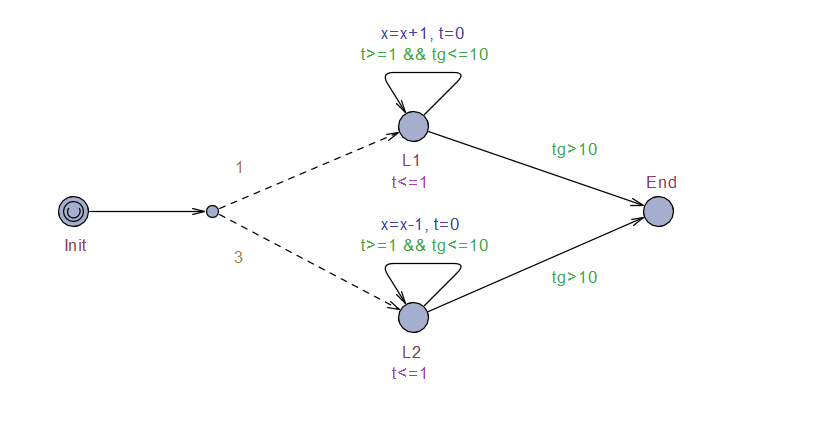
\includegraphics[scale=0.5]{./pictures/uppaal_model_example.png}
	\caption{Uppaal Model}
	\label{uppaal_Model}
\end{figure}

\begin{figure}[h]
	\centering
	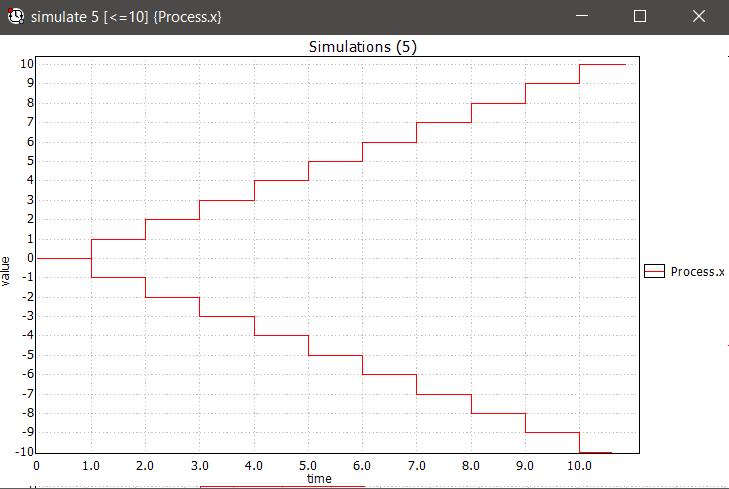
\includegraphics[scale=0.6]{./pictures/uppaal_model_example_simulation.png}
	\caption{Uppaal Simulation Trace Graph}
	\label{uppaal_Simulation_Graph}
\end{figure}

\begin{figure}[h]
	\centering
	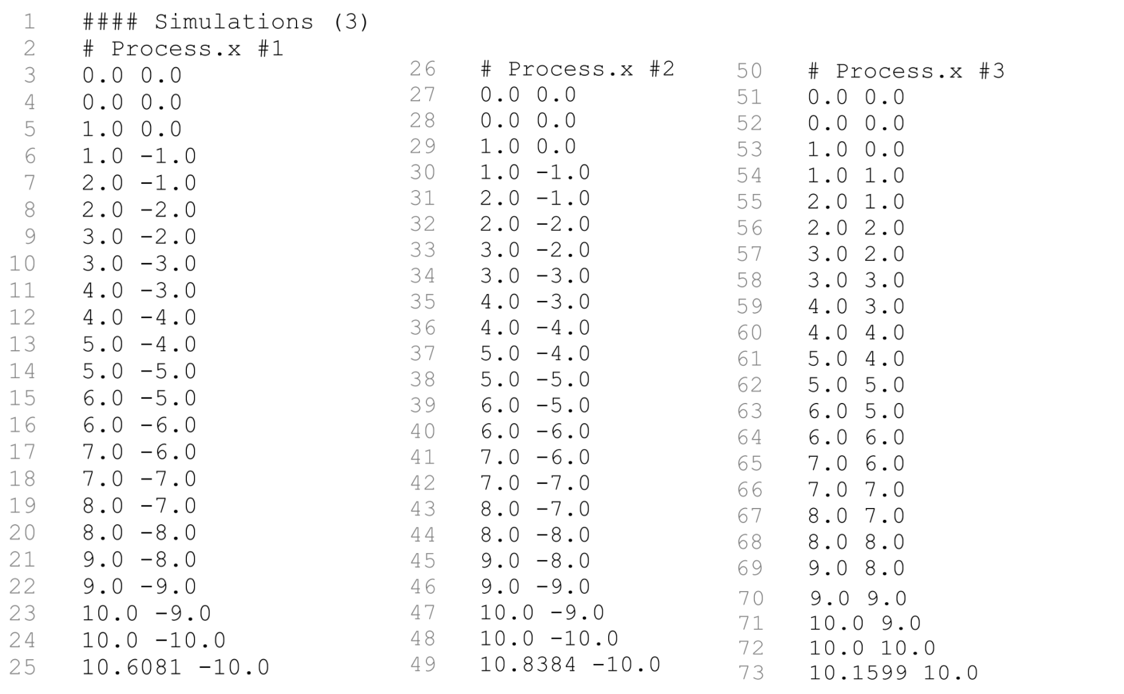
\includegraphics[scale=0.5]{./pictures/simulation_trace.png}
	\caption{Uppaal Simulation Trace Data}
	\label{uppaal_Simulation_Trace}
\end{figure}

\section{Graph Theory}
In the implementation of this project, we represent observations of system simulations as \textit{directed acyclic graphs}, also called \textit{learned models}, by applying variants of techniques like \textit{graph matching} and \textit{graph edit distance} with the incorporation of distance metrics like \textit{Euclidean distance} in an incremental fashion. Therefore we begin by giving the definition of a graph and then an overview of the previous techniques. A more detailed explanation of the mentioned subjects can bee seen in the following two papers of Vincenzo Carletti \cite{graphMatching} and Bengoetxea Endika \cite{theGraphMatchingProblem}. The first paper mainly focuses on graph edit distance and graph theory, while the other on the graph matching problem. Nevertheless, it is important to mention that the graph matching problem is categorized as NP-Complete.

\subsection{Graph Definition}
A graph is a structure $G=(V,E)$ composed of two finite sets: a node set $V$ (or vertices) that represents objects in a domain and an edge set $E \subseteq V \times V$ which represent the relationships among objects. Each edge $e \in E$ is a couple of nodes $e=(u,u')$ where the nodes connected are called \textit{adjacent}. The set $adj(u) = \{ u' \in V | \exists (u,u') \in E \}$ of the nodes adjacent to $u$ is commonly named neighborhood. If the couple $(u,u')$ is ordered, the edge $e$ is said to be directed. A \textit{directed graph} is a graph in which all edges are directed or oriented from one node to another. A directed graph is considered $acyclic$ if the directed graph has a topological ordering, such that for every directed edge $uv$ from node $u$ to node $v$, $u$ comes before $v$ in the ordering.\\ \\ \\ \\
%
Graphs can also bring semantic information by the use of labels and attributes. We take advantage of this properties to map probabilistic timed automata along their components as directed acyclic graphs.
%
\theoremstyle{definition}
\begin{definition}{(Labeled Graph)}
	A labeled graph is a tuple $G= (V,E,\mu, v)$ where
	\begin{itemize}
		\item[--]
		$L$ is a finite alphabet of nodes and edges labels.
		\item[--]
		$\mu: V \rightarrow L$ is a node labeling function. 
		\item[--]
		$v: E \rightarrow L$ is an edge labeling function.  
	\end{itemize} 
\end{definition}

\theoremstyle{definition}
\begin{definition}{(Attributed Graph)}
	Similarly, given that $\mathbb{A}$ is a set of structured information . An attributed graph is a tuple $G= (V,E,\alpha, \gamma)$ where
	\begin{itemize}
		\item[--]
		$\alpha: V \rightarrow \mathbb{A}$ is a node attribute function. 
		\item[--]
		$\gamma: E \rightarrow \mathbb{A}$ is an edge attribute function. 
	\end{itemize} 
\end{definition}


\subsection{Graph Matching}
In pattern recognition, an important problem consists of finding a mapping between the nodes and edges of two graphs, that satisfy a given set of structural constraints. Such problem is commonly known as the \textit{graph matching problem}, whose goal is to find structural correspondence between graphs. 

\subsection{Exact Matching}
\theoremstyle{definition}
\begin{definition}{(Exact graph matching)}
Given two graphs, model graph $G _{M} = (V_ {M}, E_{M})$ and data graph $G _{D} = (V_ {D}, E_{D}),$ with $|V_ {M}| = |V_ {D}|$, the problem is to find a one-to-one mapping $f : V_ {D} \rightarrow V_ {M}$ such that $(u,v) \in E_{D}$ iff $(f(u), f(v)) \in E_{M}$. When such a mapping $f$ exists, $G_D$ is said to be isomorphic to $G_M$. 
\end{definition}

\subsection{Inexact Matching} 
In some real situations the variability of the patterns, the noise in the processes or other causes, may produce deformation in the observed graphs. So two graphs may have similar structures, but with some extra or missing nodes and edges. For these cases, the conditions of exact graph matching are too strict to find out a mapping between two graphs. The most adopted solution is to make the matching process tolerant to deformations by introducing matching costs to penalize structural differences. The closer the structures of two graphs are, the lower is the cost to match them. A well known method to define the matching cost is the \textit{graph edit distance}, which assigns a cost to each operation needed to transform one graph into another one. Please refer to Fig. \ref{graph_edit_distance} for an example of the graph edit distance technique. 
%
\theoremstyle{definition}
\begin{definition}{(Graph edit operations)}
	a graph edit operation is one of the following operations applied on a graph: Node/Edge removal, Node/edge insertion, Node/Edge substitution.
\end{definition}
%
\theoremstyle{definition}
\begin{definition}{(Edit path)}
	an edit path of a graph $G$ is a sequence of elementary operations applied on $G$. It is possible to assign a cost to each simple operation. Among all possible transformations that involve two graphs $G1$ and $G2$, we are interested in the cheapest one, whose cost is the graph edit distance $d(G1,G2)$ between $G1$ and $G2$. 
\end{definition}
%
\begin{figure}[t]
	\centering
	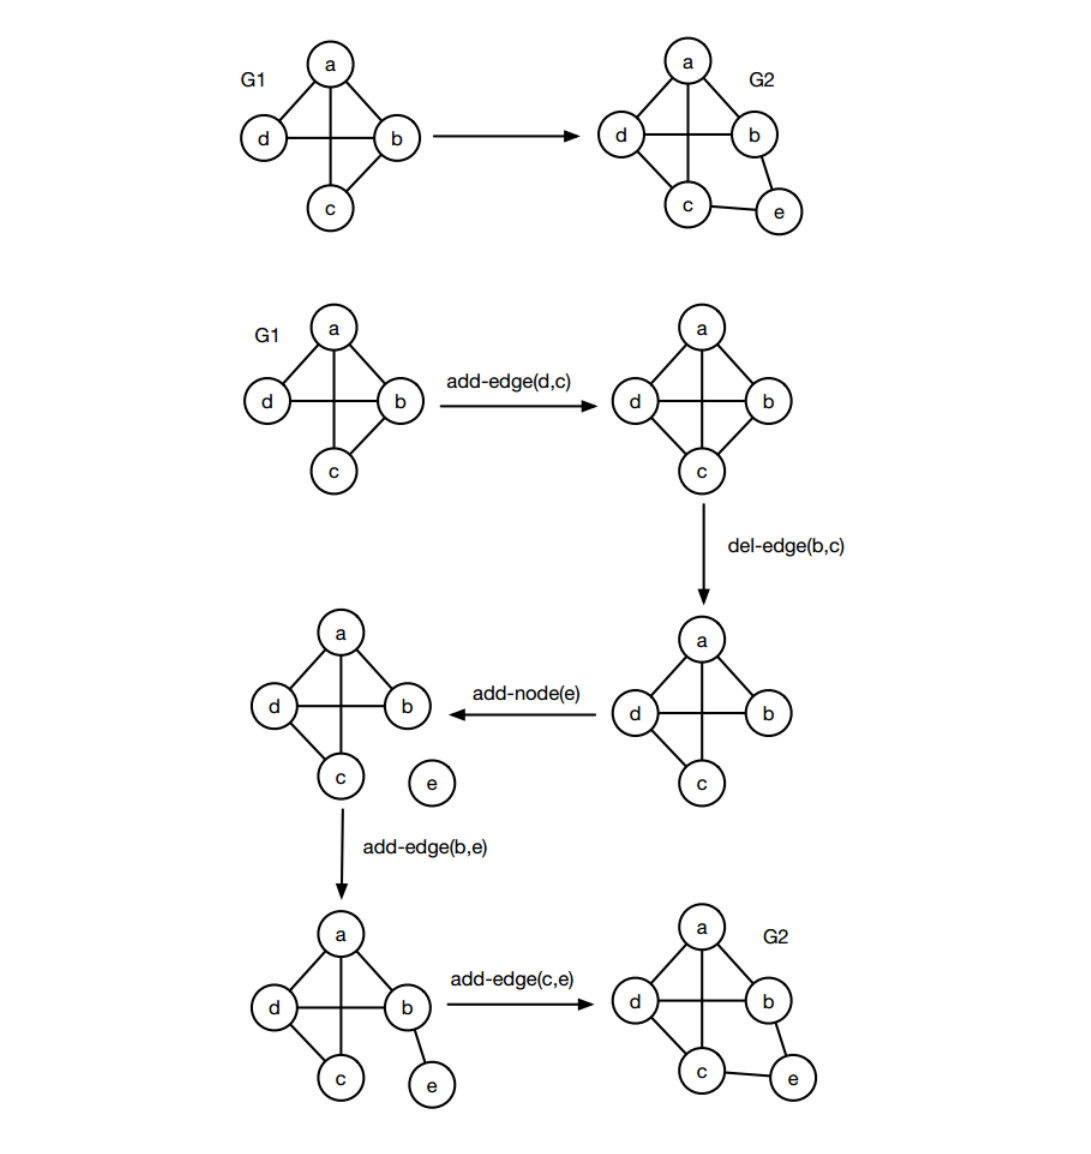
\includegraphics[scale=0.5]{./pictures/graph_edit_distance.png}
	\caption{Graph edit distance example. Illustration taken from \cite{graphMatching}}
	\label{graph_edit_distance}
\end{figure}

\subsection{The Assignment Problem} 
Graph edit distance compares two graphs with \textit{static structures} that do not change over time. We on the other hand, apply a similar approach incrementally and on the fly, as we attempt to match graphs with \textit{dynamic structures} that change over time. Despite this difference, both approaches share another problem, which is the assignment of nodes from one graph to the other. We tackle this issue by mapping the nodes of graphs with the use of the euclidean distance as a mapping function. Further details are given in \Cref{chap:incremental_Learning}
%
\theoremstyle{definition}
\begin{definition}{(Assignment)}
	an assignment is usually represented as a bijective mapping $\varphi: X \rightarrow Y$ between two finite sets $X= \{ x_i \}_i$ and $Y= \{ y_i \}_i$ of size $|X| = |Y| = n$. By assigning the $n$ elements of $X$ to the $n$ elements of $Y$ we get an assignment $\varphi$ corresponding to a permutation $(\varphi(1), \dots, \varphi(n))$, where the first element is assigned to $\varphi(1)$, the second to $\varphi(2)$ and so on.
\end{definition}

\theoremstyle{definition}
\begin{definition}{(Euclidean distance)} \cite{eucledianDistance}
	The euclidean distance or euclidean metric is the ordinary straight-line distance between two points in euclidean space. With this distance, euclidean space becomes a metric space. In Cartesian coordinates, the euclidean distance of between ponint $p=(p_1, p_2, \dots, p_n)$ and point $q=(q_1, q_2, \dots, q_n)$ is given by:
	\begin{equation}
		d(p,q) = d(q,p) = \sqrt{(q_1 - p_1)^2 + (q_2 - p_2)^2 + \dots (q_n - p_n)^2} = \sqrt{\sum_{i=1}^{n} (q_i - p_i)^2}
	\end{equation}
\end{definition}


%\section{Automata Learning}
%Generally explain how learning can be applied or used in timed automata. 
%
%\subsection{Active and Passive}
%General explanation of active and passive learning in timed automata learning. \newpage
 
	
	\chapter{Related Work}
	\label{chap:related_work}
	In this section we share a rough overview of the principal topics that inspired this paper, and that are also on-going and related research subjects. The main concepts discussed are: \textit{active automata learning}, \textit{incremental minimal construction of deterministic finite automata} and \textit{graph matching}. \\ \\
%
Despite the fact that we do not interact directly with models in our incremental learning approach, we do share similar challenges that apply to active automata learning. There is no straightforward pattern that clearly indicates the termination and correctness of learning, as seen in the paper from Howar, Falk and Steffen, Bernhard \cite{activeLearning}. In active learning, it is possible to indicate partial correctness, because learning terminates after the equivalence is guaranteed by the execution of equivalence queries. As for termination, the amount of time to learn a system remains to be proved, because the learning process highly depends on queries to the system, which execution may vary in time depending on the received observations of a system. It is to be remarked that in our incremental learning approach we are also not able to determine full correctness and termination, due to the lack of interaction with the system and the types of observation that we evaluate. Nevertheless, there exists papers in which active learning is used with simple practical examples, as seen in paper written by Steffen, Bernhard and Howar, Falk and Merten, Maik \cite{activeAtuomata}, where models are learned not only with automata, but with \textit{Mealy machines}.\\ \\
%
Incremental learning and construction of automata has been also discussed and applied to improve the efficiency and optimization of automata.
%
Our approach consists on incremental learning and measurement of probabilistic timed automaton, which is strongly related to the approaches of constructing incremental minimal automata from the book of \textit{Optimization of automata } \cite{optimizationOfAutomata}. In this book, incremental construction of minimal finite-state automata is applied in the context of natural language processing by incrementally verifying that letters of a language are recognized by the minimal possible number of states. We do not ensure in our implementation that our \textit{learned models} are minimal, but we are capable of avoiding redundant nodes by verifying the similarity of the nodes with Euclidean distances and cost functions. Minimization of automata is also a very important and related topic, because minimal automata might be easier to learn as automata with redundant nodes. There exists a great variety of algorithms for automata minimization, which are very well described in the paper \textit{Minimization of automata} \cite{minimizationOfautomata}. \\ \\
%
Graph matching, as discussed in \Cref{chap:background}, is a powerful technique that involves matching nodes and edges of two graphs. We utilize similar techniques related to graph matching like \textit{semantic matching}, which can be seen in more detailed in the paper of \textit{S-Match: an algorithm and an implementation of semantic matching} \cite{graphSemanticMatching}. In graph semantic matching, the nodes of a graph are identified by calculating the semantic relations between concepts of nodes and not their labels. This is a very interesting concept that we applied by labeling nodes depending on their functionalities, with the use of Euclidean distances. 
%
Graph matching itself is a very wide and complicated topic that has been applied in many areas of the real world. One example can be web search engines, in which nodes and edges of enormous graphs are coupled by relating and categorizing sources or information of graphs by hubs and authorities, explained in paper the paper of \textit{Graph similarity scoring and matching} \cite{graphSimilarityScoringMatching}. Other interesting areas are: image analysis, biometric identification, video analysis, document processing, among others, very well explained in the paper of \textit{Thirty years of graph matching in pattern recognition} \cite{patternRecognition}. 
%

	
	\chapter{Incremental Learning}	
	\label{chap:incremental_Learning}
	The learning process of a system begins by analyzing a \textit{trace} from a simulation.
%
A trace is a set of \textit{observations} from which \textit{equations} are derived, by fitting the trend of the data to mathematical functions.
%
Each equation represents a \textit{functionality} with knowledge to be incorporated into a \textit{learned model} as a \textit{node}. 
%
We use an \textit{incremental learning} approach, as each node to be incorporated is priorly \textit{measured} or evaluated in terms of cost with respect to the learned model.
%
Simultaneously, the structure of the learned model is matched against the one from the observed system, only to indicate the progress of the learning process. \\ \\
%
In this chapter we discuss how incremental learning works by first explaining how the data from observations is fitted to equations in the \textit{Data Fitting} section. Then we describe how the equations are used to learn information in section \textit{Data Learning}. We discuss how learned data is modeled in section \textit{Data Modelling}, and in the last section \textit{Cost Evaluation}, we explain how the use of costs influence the modelling and learning of data. 

\section{Data Fitting}
We consider an \textit{observation} as the value of a variable in an exact time, obtained from a simulation trace.
%
By gathering more than one observation and fitting the curve of the data, we are able to derive equations that express the  \textit{behavior} of a variable given a period of time. 
%
The procedure is implemented by storing the data of a trace using a \textit{buffer} (e.g. \ref{buffer_slide}) structure, that gathers observations from a simulation trace, which are later fitted to equations, as seen in algorithm \ref{dataFitter}. The buffer gathers observations, as long as the trace was not fully traversed (line number 2). The information of the \textit{buffer} was designed as a \textit{Map} in such way that the exact \textit{time} and \textit{value} of an observation can be extracted from it (lines 3-7). Once all observations were extracted from the \textit{buffer}, they are fitted and stored as equations in a list of equations (lines 8-9).
%
\begin{algorithm}
	\caption{Data-Fitter}
	\label{dataFitter}
	\begin{algorithmic}[1]
		\Procedure{fitdata}{timeStep, buffer, traceData}
		
		\While{$ windowSlideLimit == false $}
%		
%		\State $lastEquationFits \gets evaluateLastEquation(\vars{buffer})$
%		
%		\If{ $lastEquationFits = true$}
%			\State $updateLastEquationsConstraint(\vars{buffer})$
%		\Else
		
		\ForEach{$entry \in buffer $}
			\State $time\gets entry.getKey()$
			\State $value\gets entry.getValue()$
			\State $observations.add(time,value)$
		\EndFor
		
		\State $equation\gets \func{fitEquation}(\vars{observations})$
		\State $\func{equationsList.add}(\vars{equation})$
		
%		\EndIf
		
		\State $ windowSlideLimit \gets \func{slideBuffer}(\vars{timeStep, traceData})$
		
		\EndWhile
		
		\EndProcedure
	\end{algorithmic}
\end{algorithm}
	 
%
\begin{figure}[h]
\begin{center}
		\begin{tabular}{||c c ||}
		\hline
		Time & Value  \\ [0.5ex] 
		\hline\hline
		\textbf{0} & \textbf{1} \\ 
		\hline
		\textbf{1} & \textbf{2} \\
		\hline
		\textbf{2} & \textbf{3} \\
		\hline
		3 & 4 \\
		\hline
		4 & 5  \\ [1ex] 
		\hline
	\end{tabular}
	\begin{tabular}{||c c ||}
		\hline
		Time & Value  \\ [0.5ex] 
		\hline\hline
		 0 & 1 \\ 
		\hline
		\textbf{1} & \textbf{2} \\
		\hline
		\textbf{2} & \textbf{3} \\
		\hline
		\textbf{3} & \textbf{4} \\
		\hline
		4 & 5  \\ [1ex] 
		\hline
	\end{tabular}
	\begin{tabular}{||c c ||}
		\hline
		Time & Value  \\ [0.5ex] 
		\hline\hline
		0 & 1 \\ 
		\hline
		1 & 2 \\
		\hline
		\textbf{2} & \textbf{3} \\
		\hline
		\textbf{3} & \textbf{4} \\
		\hline
		\textbf{4} & \textbf{5}  \\ [1ex] 
		\hline
	\end{tabular}
\end{center}
\caption{Example of buffer storing information of a trace}
\label{buffer_slide}
\end{figure}

\section{Data Learning}
Given that each equation trace is organized by time and that the initial node of the learned model \textit{lm} is known.
%
For each equation in an equation trace, we proceed to traverse the learned model to measure the similarity between existing neighbor nodes or \textit{direct successors} and the observed equation. 
%
An equation is incorporated to the model depending on the distance that it has among the direct successors (if any), and the knowledge that we obtain from it, as seen in Algorithm \ref{learner}.
%
\begin{algorithm}
	\caption{Learner}
	\label{learner}
	\begin{algorithmic}[1]
		\Procedure{learner}{equationTrace}

			\State $parent \gets lm.getInitialLocation()$
			
			\ForEach {$equation \in equationTrace $}
			
				\State $directSuccessors \gets lm.getDirectSuccessors(\vars{parent})$
				
				\If{$directSuccessors.length>0$}
					\State $distances \gets \func{measureDistances(\vars{directSuccessors,equation})}$
					\State $lastModifiedNode \gets \func{incrementalLearning(\vars{distances})}$
				\Else
					\State $lastModifiedNode \gets \func{addNodeToLearnedModel(\vars{equation})}$
%					\State $Mark\_node\_as\_not\_learned$
				\EndIf
				
				\State $parent \gets \vars{lastModifiedNode}$
				
			\EndFor
			
		\EndProcedure
	\end{algorithmic}
\end{algorithm}


%
\subsection{Measuring Distance}
The similarity between direct successors and an observed equation is measured based on Euclidean distance with Algorithm \ref{measureDistances}. Given that \textit{time steps} represent the time range in which an equation was observed. For each \textit{neighbor} among the direct successors, we evaluate the fitted function of the observed equation \textit{observed function} and the one from the neighbor \textit{neighbor function} to obtain the two sets of points \textit{observed points} and \textit{neighbor points}, which will later be used to obtain the \textit{Euclidean distance}. It is important to note that the euclidean distance is normalized to a value between 0 and 1 in line 10 of the algorithm, and that we perform the same procedure for every neighbor and store every distance in the list \textit{distance list}. 
%
\begin{algorithm}
%	\caption{Get Distances. The distance is the euclidean distance between the values of the observed equation and a neighbor's equation, after both were evaluated with the time steps of the observed equation. 
%		\newline \textbf{Input}: Direct successors and an observed equation. 
%		\newline \textbf{Output}: List of the distance of all neighbors with respect to the observation. }
	\caption{Measure-Distances}
	\label{measureDistances}
	\begin{algorithmic}[1]
		\Procedure{measure-distances}{directSuccessors, observedEquation}
		
		\State $timeSteps\gets \vars{observedEquation.timeSteps}$
		\State $observedFunction\gets \vars{observedEquation.fittedFunction}$
		
		\ForEach {$neighbor \in directSuccessors$}
			\State $neighborFunction\gets \vars{neighbor.fittedFunction}$
			\State $neighborPoints \gets \func{evaluatefunction(\vars{neighborFunction, timeSteps})}$
			\State $observedPoints \gets \func{evaluatefunction(\vars{observedFunction, timeSteps})}$
			\State $distance \gets \func{getEuclideanDistance(\vars{observedPoints, neighborPoints})}$
			\State $distance \gets 1/(1+distance)$
			\State $distanceList.push(distance)$
		\EndFor
		
		\State \Return $distanceList$
	
		\EndProcedure
	\end{algorithmic}
\end{algorithm}



\section{Data Modelling}
We attempt to merge similar observations to avoid redundant or unnecessary nodes in our learned model, by using the gathered distances from Algorithm \ref{measureDistances}. 
%
Among all distances, we retrieve the node with the closest distance (\textit{closest node}) that satisfies our similarity criteria (\textit{similarity threshold}), with the intention of evaluating the cost of adding a similar observation as a \textit{new node} or as a \textit{merged node}. If an observation does not satisfy the similarity threshold, then the closest node below the threshold (\textit{far node}) is retrieved and added to the learned model as a new location. As depicted in Algorithm \ref{incrementalLearning}.
%
\begin{algorithm}
	\caption{Incremental-Learning. An observed equation is added to the learned model as a new node or as a merged node, based on the closeness that it has among direct successors.
	\newline Input: similarity threshold \textit{sim\_th}, given by the user}
%	\caption{Incremental-Learning}
	\label{incrementalLearning}
	\begin{algorithmic}[1]
		\Procedure{Incremental-Learning}{distances, observedEquation}
		
		\State $closestNode \gets \func{getClosestDistanceAboveThreshold(\vars{distances, sim\_th})}$
		\State $farNode \gets \func{getClosestDistanceBelowThreshold(\vars{distances, sim\_th})}$
		
		\If {closestNode.isNotEmpty()}
			\State $nextNode \gets \func{addLeastExpensiveChange(\vars{closestNode, observedEquation})}$
			\State	\Return $nextNodeToTraverse$
		\EndIf
		
		\If {farNode.isNotEmpty()}
			\State $nextNode \gets \func{addNodeToLearnedModel(\vars{farNode, observedEquation})}$
			\State	\Return $nextNode$
		\EndIf
	
		\EndProcedure
	\end{algorithmic}
\end{algorithm}



%
\section{Cost Evaluation}
%
The gathered knowledge of a system is always resembled by the latest structure and functionality of the learned model. An observed equation represents new knowledge, which we would like to incorporate to our learned model. The way that we evaluate this incorporation is by estimating the cost of the following points: Number of nodes required to express the information in the learned model (either as a new node or a replacement), plus the error that it may transmit or propagate to other relevant close nodes from the learned model, as seen in Equation \ref{cost}.
\begin{equation} 
\label{cost}
	Cost = nodeCount*nodeCost + propagation
\end{equation}
%
Based on the previous general cost function, we derive two types of cost functions to decide whether to add or replace nodes: \textit{replacement cost} and \textit{addition cost}, where we always conclude that the function with the lowest cost is the one that determines how an observed equation will be incorporated to the learned model. \\ \\
%
For explanation purposes, we will be making the following assumptions: 1) The Uppaal model from Figure \ref{learned_model_example} represents our learned model, 2) We have observed an equation $x=x+1$ from times \textit{0-10} of a simulation and wish to incorporate it to the model by utilizing cost functions. 
%
\begin{figure}[h]
	\centering
	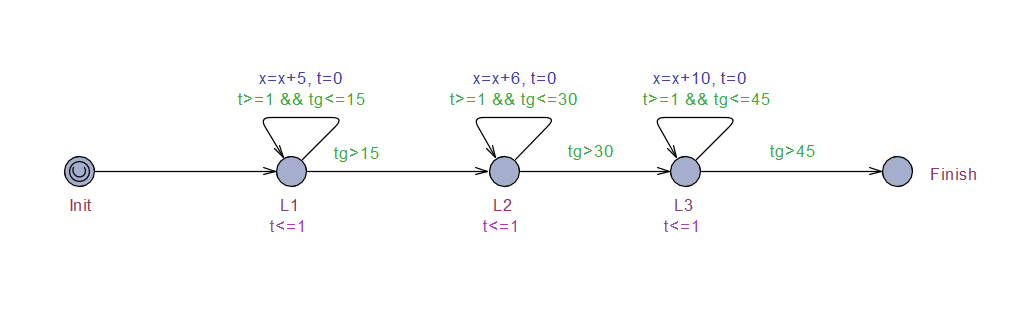
\includegraphics[scale=0.5]{./pictures/learned_model_example.png}
	\caption{Learned model example}
	\label{learned_model_example}
\end{figure}

\subsection{Addition Cost}
The addition of an observation consists of adding a node to the learned model without modifying other nodes functionalities and time constraints. The only cost for this change is determined by the \textit{addition cost}, thus the function cost for this case is determined by: $additionCost = nodeCost$. \\ \\
%
An example of adding the assumed observation as a new node to the learned model can be seen in Figure \ref{learned_model_example_addition}. 
%
\begin{figure}[t]
	\centering
	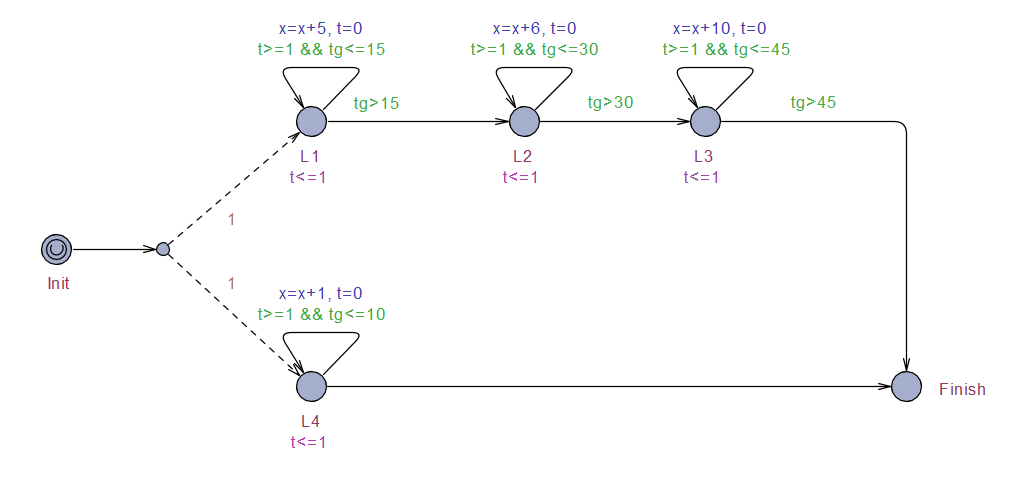
\includegraphics[scale=0.5]{./pictures/learned_model_example_addition.png}
	\caption{Node addition to learned model example}
	\label{learned_model_example_addition}
\end{figure}

\subsection{Replacement Cost}
The replacement of a node in the learned model consists of merging the functionality and time constraints of an observation with the ones from a node, without adding extra nodes. The cost of this change is mainly determined by two types of propagation:  functionality propagation ($propagation_f$) and time propagation ($propagation_t$):
%
\begin{equation}
replacementCost = propagation_f*functionalityCost + propagation_t* timeCost,
\end{equation}
where the first propagation represents how the modification of the functionality of a node can affect the distance of other nodes, while the second represents how modifying time constraints can affect other nodes. We will explain how location $L1$ is merged with the observation in the following subsections. 

\subsection{Time Propagation}
The already learned time constraints of $L1$ state that the location should be active for 15 seconds of the simulation and then take the edge to location $L2$. We have observed a functionality with a duration of 10 seconds (5 seconds less than $L1$). The possibilities of merging the time constraints of both the observation and $L1$ are given by the following cases:
\begin{itemize}
	\item Ignoring: We decide to ignore that we observed 5 seconds of the observation (e.g. times from 10 - 15) and not modify the time constraints of $L1$. 
	\item Updating: We decide to modify the time constraints of $L1$, as depicted in Figure \ref{learned_model_example_time_replacement}.
	\item Splitting: We decide to not modify the time constraints of $L1$ and add extra locations from the constraints that were not satisfied by $L1$. For this, we evaluate the time of the location $L1$ and the time of the observation $Obs$ as sets, and add locations according to the difference of the time sets. An example can be seen in Figure \ref{learned_model_example_time_replacement_addition})
%	\item Splitting: we decide to modify the time constraints of $L1$ and add a second location $L1'$, in which $L1$ will have the time constraints that satisfy the ones from  the observation and $L1'$ the ones that constraint that were not satisfied. 
%	  and penalize that we subtracted 5 times of activity of $L1$. 
\end{itemize}

\begin{figure}[h]
	\centering		
	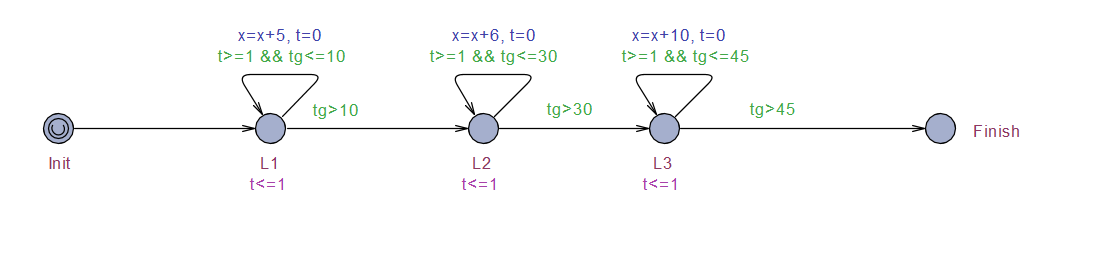
\includegraphics[scale=0.5]{./pictures/learned_model_example_time_replacement.png}
	\caption{Time constraints replacement in learned model example}
	\label{learned_model_example_time_replacement}
\end{figure}

\begin{figure}[h]
	\centering
	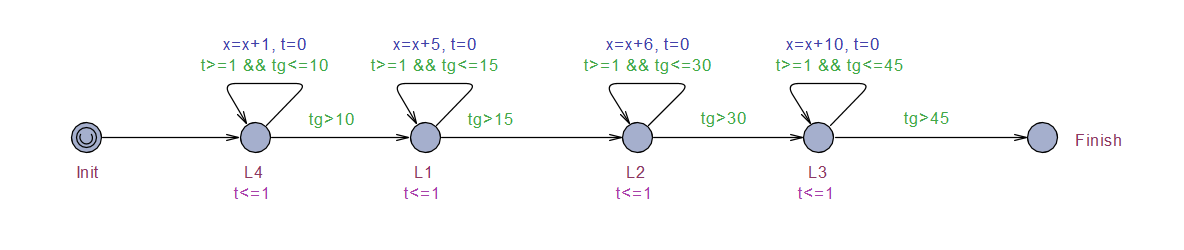
\includegraphics[scale=0.5]{./pictures/learned_model_example_time_replacement_addition.png}
	\caption{Time constraints replacement with extra location in learned model example}
	\label{learned_model_example_time_replacement_addition}
\end{figure}
%
%splitting case can be explained with a set. \\ \\
%
% Definition of circles
%\def\firstcircle{(0,0) circle (1.5cm)}
%\def\secondcircle{(0:2cm) circle (1.5cm)}
%
%\colorlet{circle edge}{blue!50}
%\colorlet{circle area}{blue!20}
%
%\tikzset{filled/.style={fill=circle area, draw=circle edge, thick},
%	outline/.style={draw=circle edge, thick}}
%
%\setlength{\parskip}{5mm}
%% Set A and B
%\begin{tikzpicture}
%\label{time_diagram}
%\begin{scope}
%\clip \firstcircle;
%\secondcircle;
%\end{scope}
%\draw[outline] \firstcircle node {$L1$};
%\draw[outline] \secondcircle node {$Obs$};
%\node[anchor=south] at (current bounding box.north) {Times analyzis};
%\end{tikzpicture}
%
%
For the first two cases, the $propagation_t$ cost is represented by the number of unseen times, which is 5, multiplied by the \textit{time cost}. The only time that the $propagation_t$ is zero, is in the last case when a location is added to keep the time constraints intact. Nevertheless, this last change causes the replacement cost to be raised by adding an additional location required to satisfy the observed time constraints. 

\subsection{Functionality Propagation}
Assuming that we want to merge the functionality of location $L1$ ($x=x+5$) with the observed functionality ($x=x+1$), we need to obtain a new fitted function. For this, we utilized the same fitting methodology as shown in Algorithm \ref{dataFitter}. We retrieve two sets of points by evaluating both functions in the same range of time and obtain the new fitted function (e.g. $x=x+3$). Once the new fitted functionality is replaced in $L1$, the $functionalityPropagation$ is determined by the difference of the Euclidean distance between the new functionality and the functionality of $L1$, along with the one from its direct successors. The result of the change  can be seen in Figure \ref{learned_model_example_time_replacement_functionality}. \\ \\
%
In this particular type of replacement, two aspects are considered:
\begin{itemize}
	\item Substitution: In this case we consider how close is the Euclidean distance of the new functionality compared to the one that was substituted. 
	\item Propagation: Here we perform the same comparison as in the previous case, but we now compare how the Euclidean distance of each direct neighbor is affected by the substituted location.
\end{itemize}
%
For the example in Figure \ref{learned_model_example_time_replacement_functionality}, we can clearly see that changing the functionality of location \textit{L1} from $x=x+5$ to $x=x+3$ has a negative effect, as the new functionality $x=x+3$ is distanced from $x=x+5$ and even more distanced from $x=x+6$. The main goal of this calculation is to consider how changing the functionality of a location can impact not only the location itself, but also others around it. 
\begin{figure}[h]
	\centering
	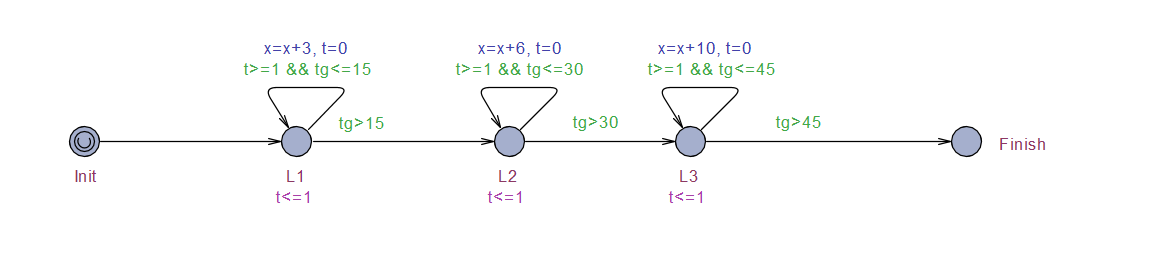
\includegraphics[scale=0.5]{./pictures/learned_model_example_replacement_functionality.png}
	\caption{Replacement of the functionality of a location in the learned model example}
	\label{learned_model_example_time_replacement_functionality}
\end{figure}

%learned_model_example_replacement_functionality

%\section{Graph Matching and Similarity Scoring}






 
	
	\chapter{Implementation}
	\label{chap:implementation}
	%The implementation of this project was created with the use of the \textit{JavaScript} open source libraries of \textit{React} and \textit{Redux}. 
%
The implementation of this project was developed as a web application. The \textit{front-end} or \textit{user interface} utilizes the \textit{JavaScript} open source library of \textit{React}. 
%
The \textit{back-end} was developed in \textit{JavaScript ES6}, and it utilizes the state management tool \textit{redux} to communicate with the \textit{front-end}. \\ \\
%
The web application mainly consists of four dependent \textit{React Components} named: \texttt{Data Manager}, \texttt{Fitting Manager}, \texttt{Learning Manager} and \texttt{Graph Matcher}. 
%
In this chapter we will explain how the components communicate between each other, and how they are used as routine to perform incremental analysis of system observations. 
%
%As \textit{React} projects are developed with the use of components, in this chapter we will discuss the main components (\textit{Data Manager}, \textit{Fitting Manager}, \textit{Learner}, \textit{Graph Matcher}) and data structures of the developed application for incremental learning.
%
%Use screenshots of the tool visual aid. 
%

\section{Data Manager}
As mentioned in \Cref{chap:incremental_Learning}, incremental learning begins by obtaining simulation data of an observed system. 
%
The \texttt{Data Manager}, which is the first section of our tool,  is in charge of organizing the data of simulations.
%
A simulation trace file from Uppaal can be imported and also visualized in the tool, as seen in the \textit{Data Plotted} from Figure \ref{data_manager}.
%
The information from the trace is parsed in this component as an \textit{array} of \textit{Map} objects that contain the points of the data per simulation run. 
%
The user can also pick the desired \textit{buffer size} and \textit{time step} value, which is going to be delivered to the \texttt{Fitting Manager}, along with the previous information for further analysis.
%
\begin{figure}[h]
	\centering
	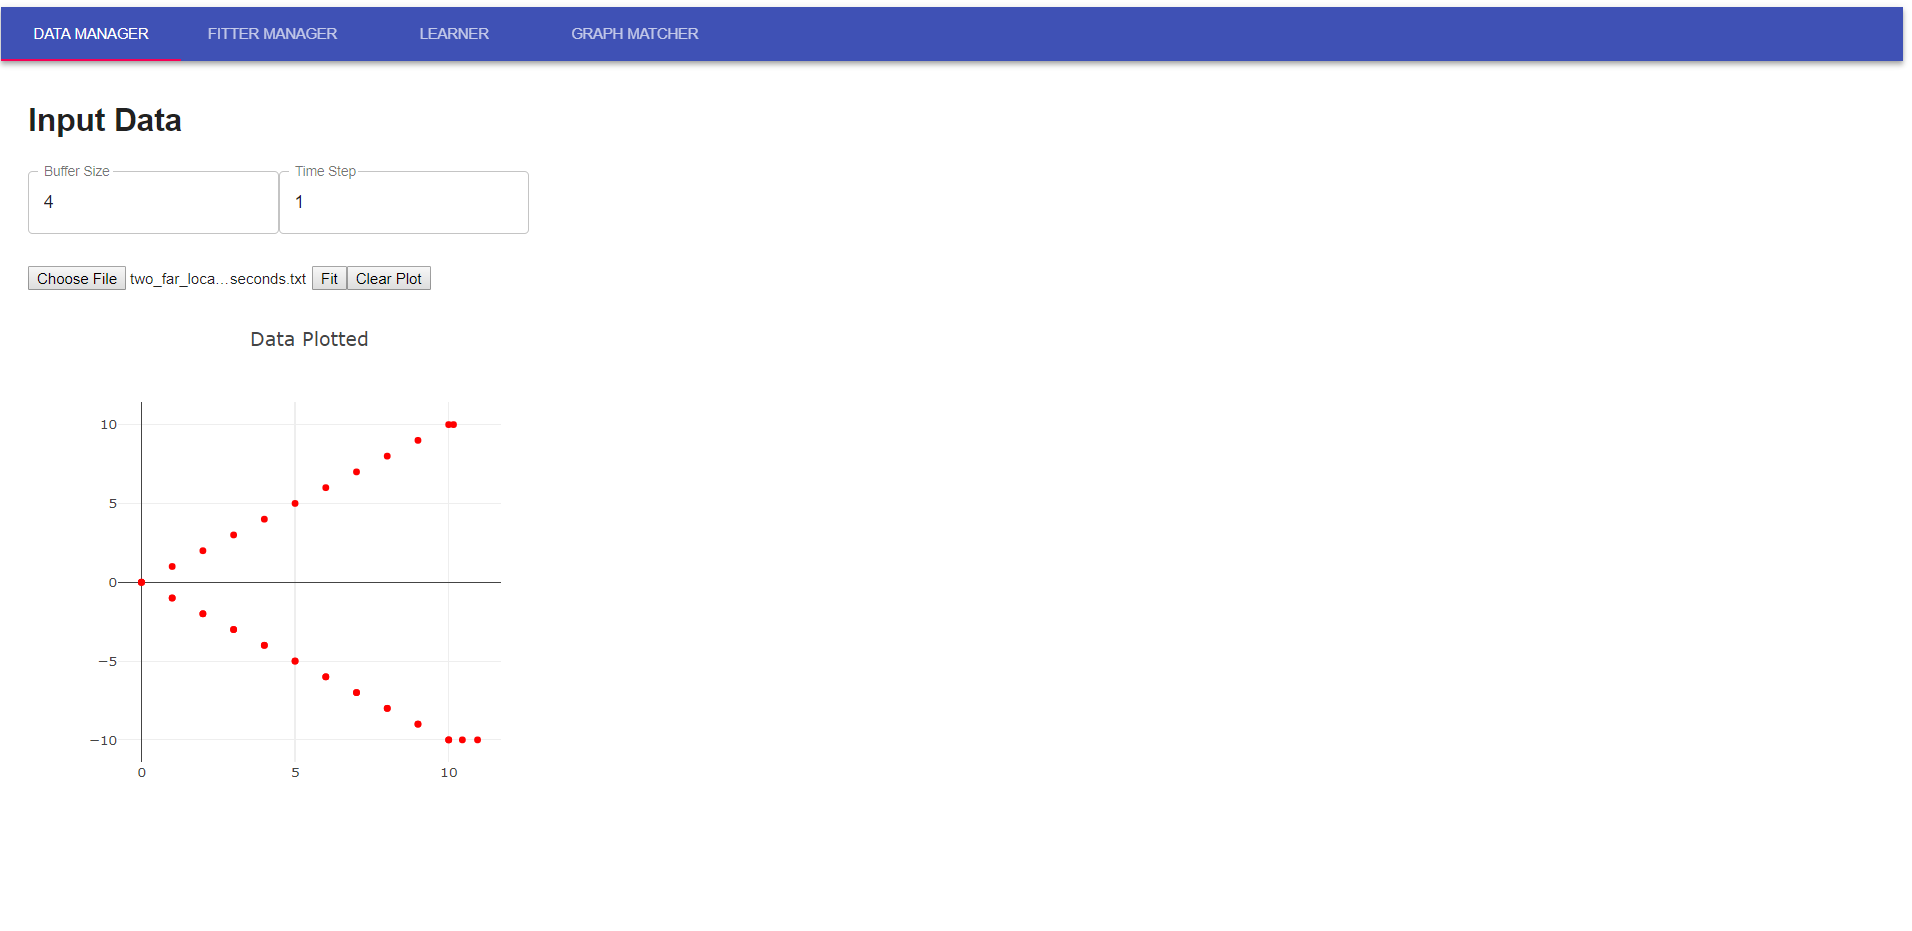
\includegraphics[scale=0.35]{./pictures/implementation/data_manager.png}
	\caption{Implementation Data Manager}
	\label{data_manager}
\end{figure}

\newpage

\section{Fitter Manager}
Given an array of maps created by the \texttt{Data Manager}, the \texttt{Fitter Manager} is in charge of fitting the observations from each map by utilizing Algorithm \ref{dataFitter} and the \textit{ml-levenberg-marquardt} library, to transform the array of maps into an array of \texttt{Equations} (structure shown in Figure \ref{equation_Structure}) which represent the behavior of an observed system, as seen in Figure \ref{fitter_manager} \\ \\
%
One can see in the \textit{Fitted Functions} text area, the results of fitting the information of each \textit{Simulation run}.
%
For every simulation run, there exists a section that contains the details of each fitted \texttt{Equation}. Let us take as an example the first fitted equation from \textit{Simulation 0}. The general information of the equation is written in black and contains the name of the equation (\textit{EQ1}), followed by the function structure ($ax+b$), the type of function that was fitted (\textit{linear}), and the \textit{Start-time} and \textit{End-Time}, that represent the range of time in which the observations were fitted. The details written in gray show the parameters that were fitted by the \textit{ml-levenberg-marquardt} library to evaluate the function, along with error of the calculations (\textit{Regression error}), that reflect the suitability of the fitted function with respect to the observed values.  
\begin{figure}[h]
	\centering
	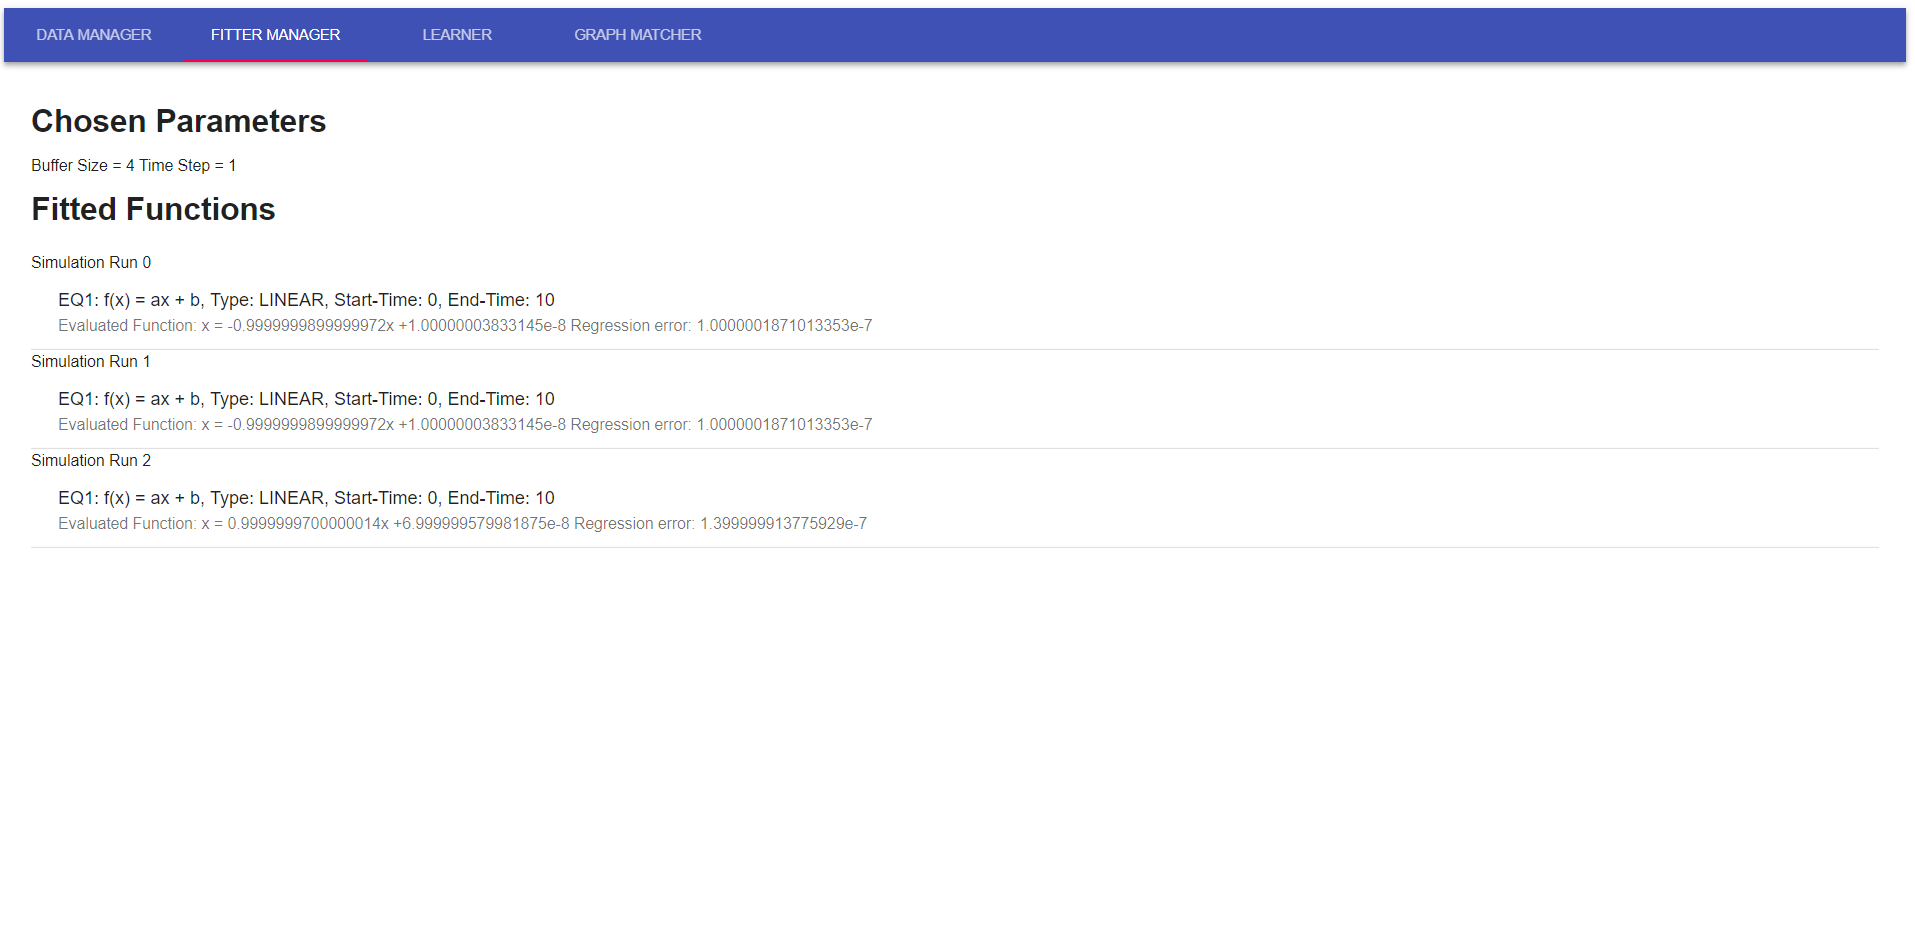
\includegraphics[scale=0.5]{./pictures/implementation/fitter_manager.png}
	\caption{Implementation Fitter Manager }
	\label{fitter_manager}
\end{figure}
\begin{figure}[t]
	\centering
	\begin{tikzpicture} 
	\umlclass{Equation}{ 
		id : string\\
		fittedFunction : string\\
		startTime : double\\
		endTime : double\\
	}{ } 
	\end{tikzpicture}
		\caption{Structure of an equation object}
	\label{equation_Structure}
\end{figure} 
 
\newpage
 
\section{Learning Manager}
%Explain in detail each cost evaluation and of how we decide to stop learning and jump to comparing or matching. 
The \texttt{Learning Manager} is responsible to perform the incremental learning approach, as explained in \Cref{chap:incremental_Learning}, with the values of the parameters that the user selects. By default, the \textit{Similarity Threshold} is set to 0.5, \textit{Time Cost} to 0.1, \textit{Functionality Cost} to 0.1 and \textit{Location Cost} to 0.5. Due to the fact that normalized Euclidean distance values between the range of zero and one are used in the incremental learning approach, we allowed to change the values of each parameter by this same range. One can also restrict the possible values of the parameters to a set of numbers (e.g. by choosing an option from the check-boxes) and learn observations for each possible combination.  
\\ \\
The tool begins the learning process after the user clicks the \textit{Learn} button. There exists two types of learning that the tool may perform: 1) With a model to reference, or 2) Without a model to reference. For the first approach, one can learn observations from systems but without evaluating the learning progress, as there is no possibility to interact with a model that resembles the observed system. Whereas in the second approach, one can import a model that resembles the observed system (e.g. Original model) producing the observations, so that the similarity of the models can also be measured \textit{on-the-fly}. Nevertheless, it is possible for both types of learning to visualize the evolution of the learned model, by selecting the desired model from the \textit{Learned Models} drop-down list. It is also important to notice that the models are constructed as directed acyclic graphs, with the only exception that \textit{self-loops} are allowed, as seen in in Figure \ref{learning_manager}. 
%
\begin{figure}[h]
	\centering
	\makebox[\textwidth][c]{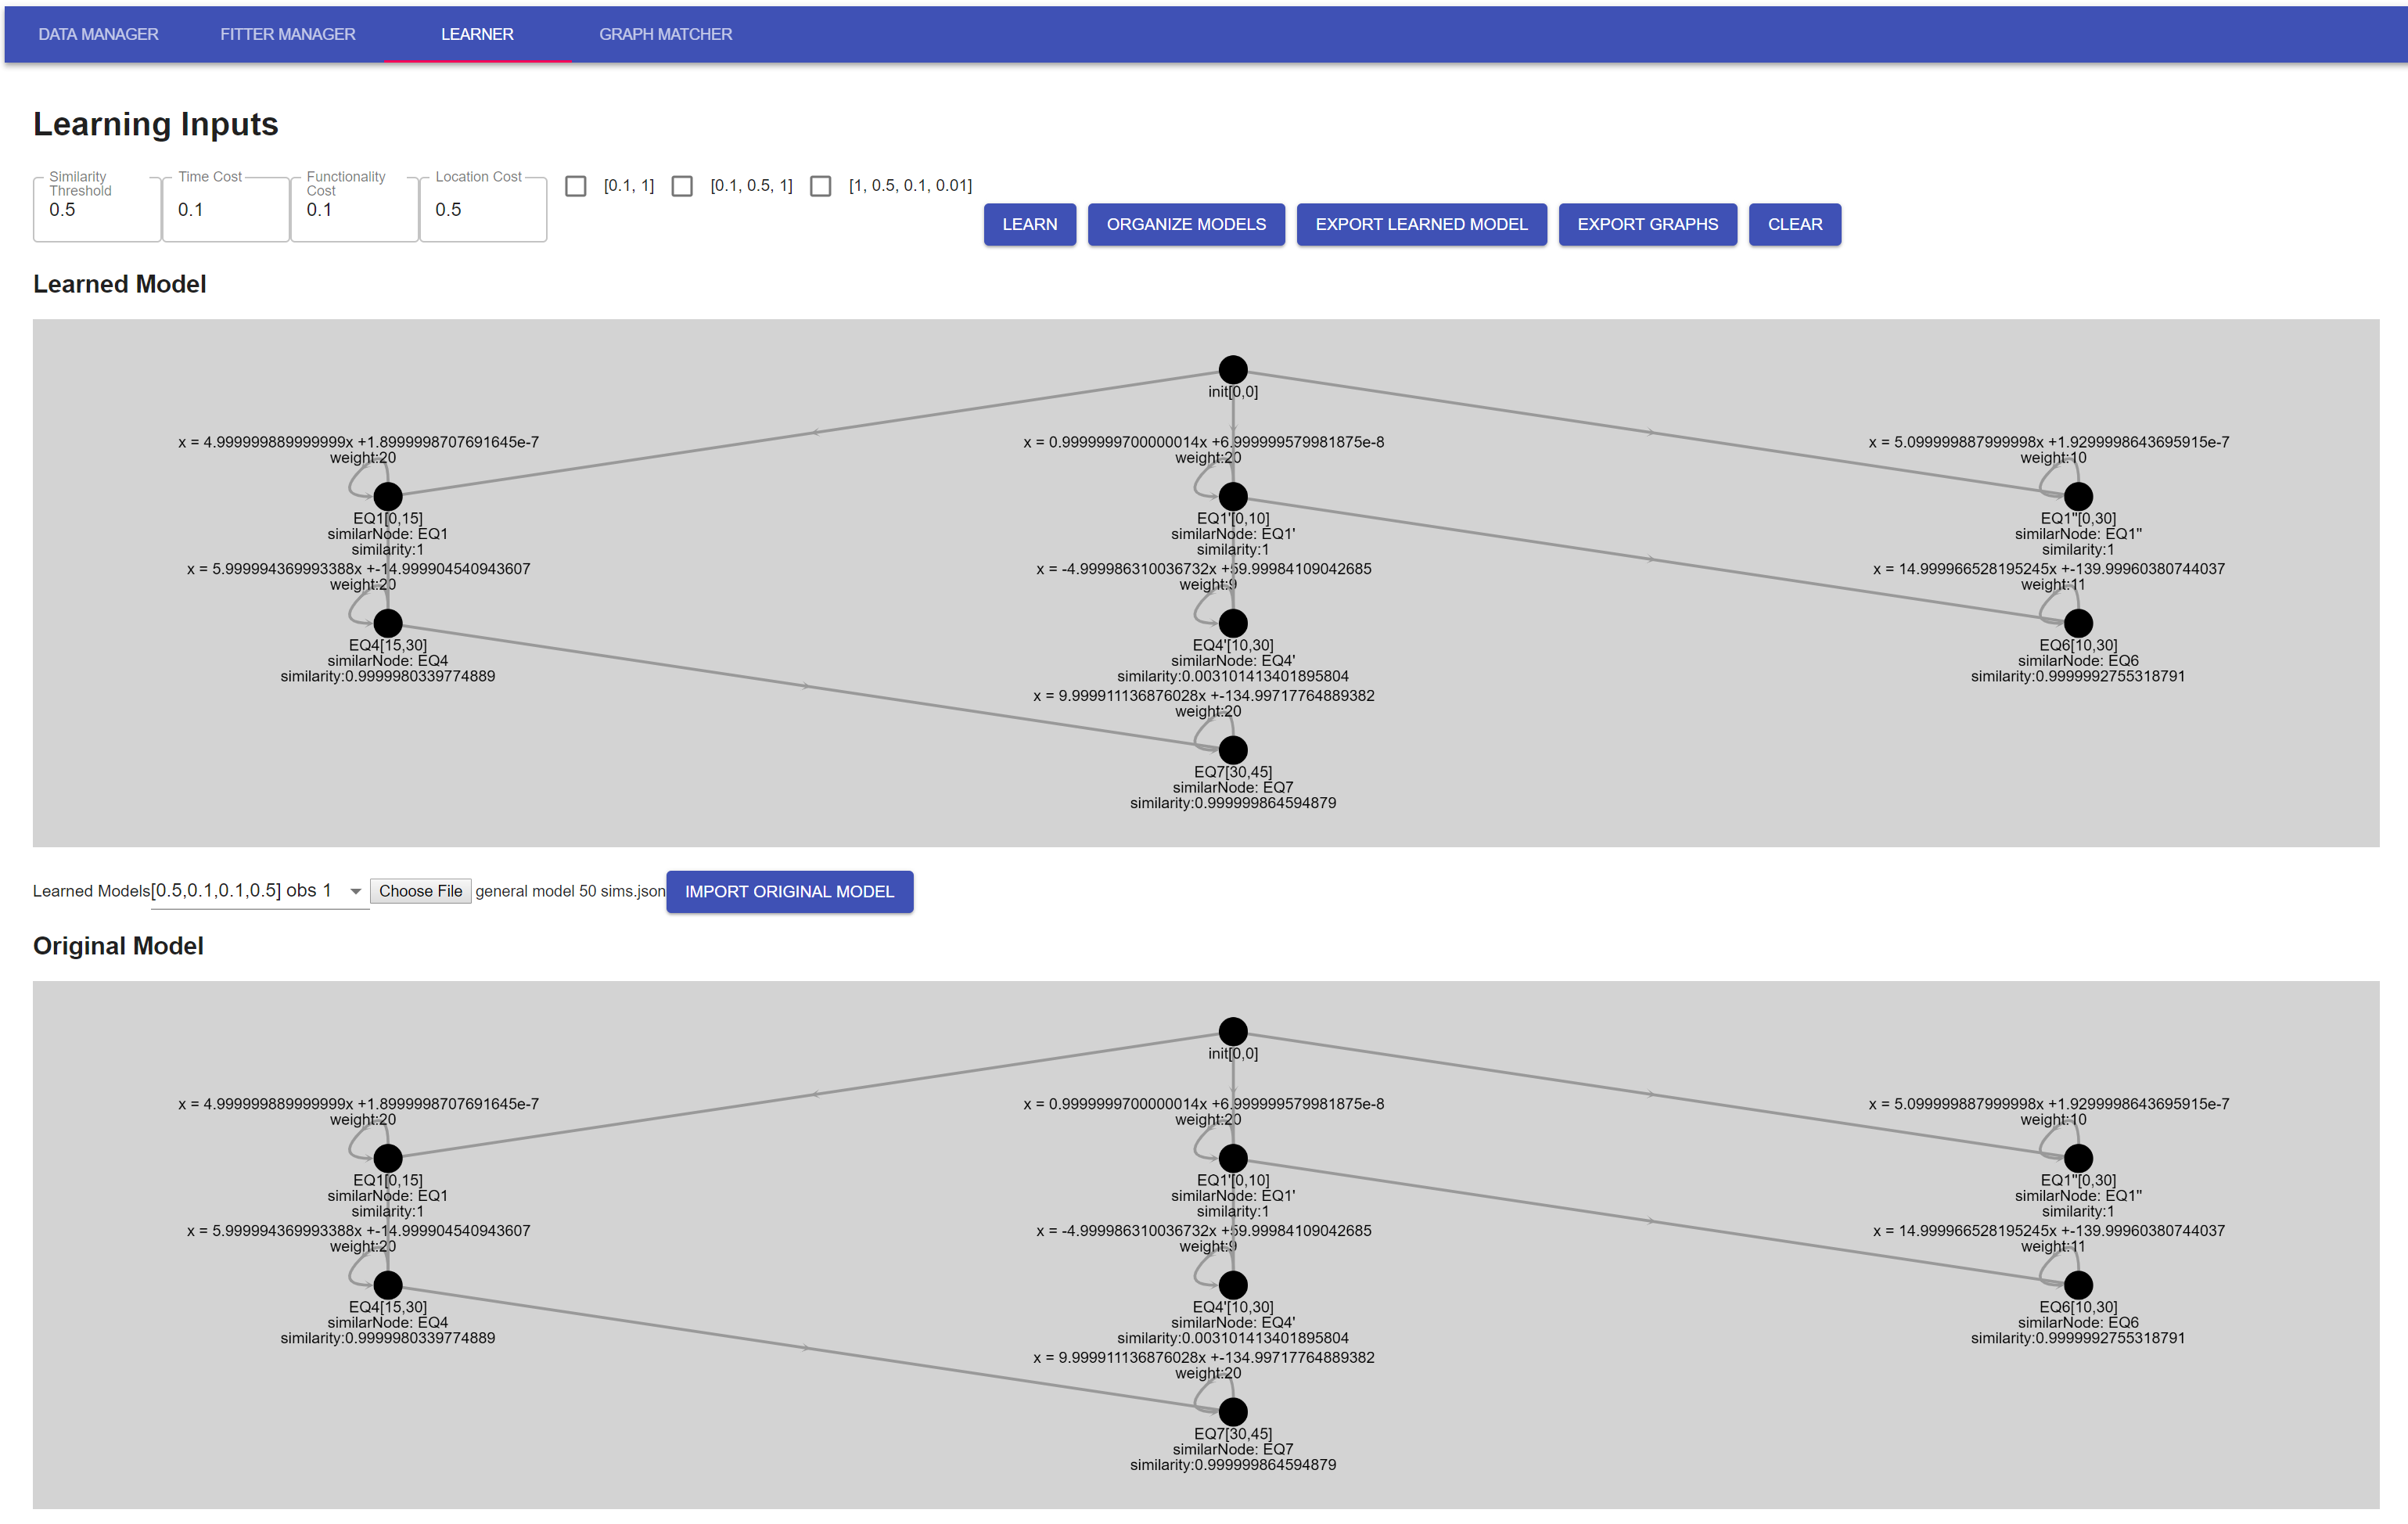
\includegraphics[width=1.1\textwidth]{./pictures/implementation/learning_manager.png}}%
%	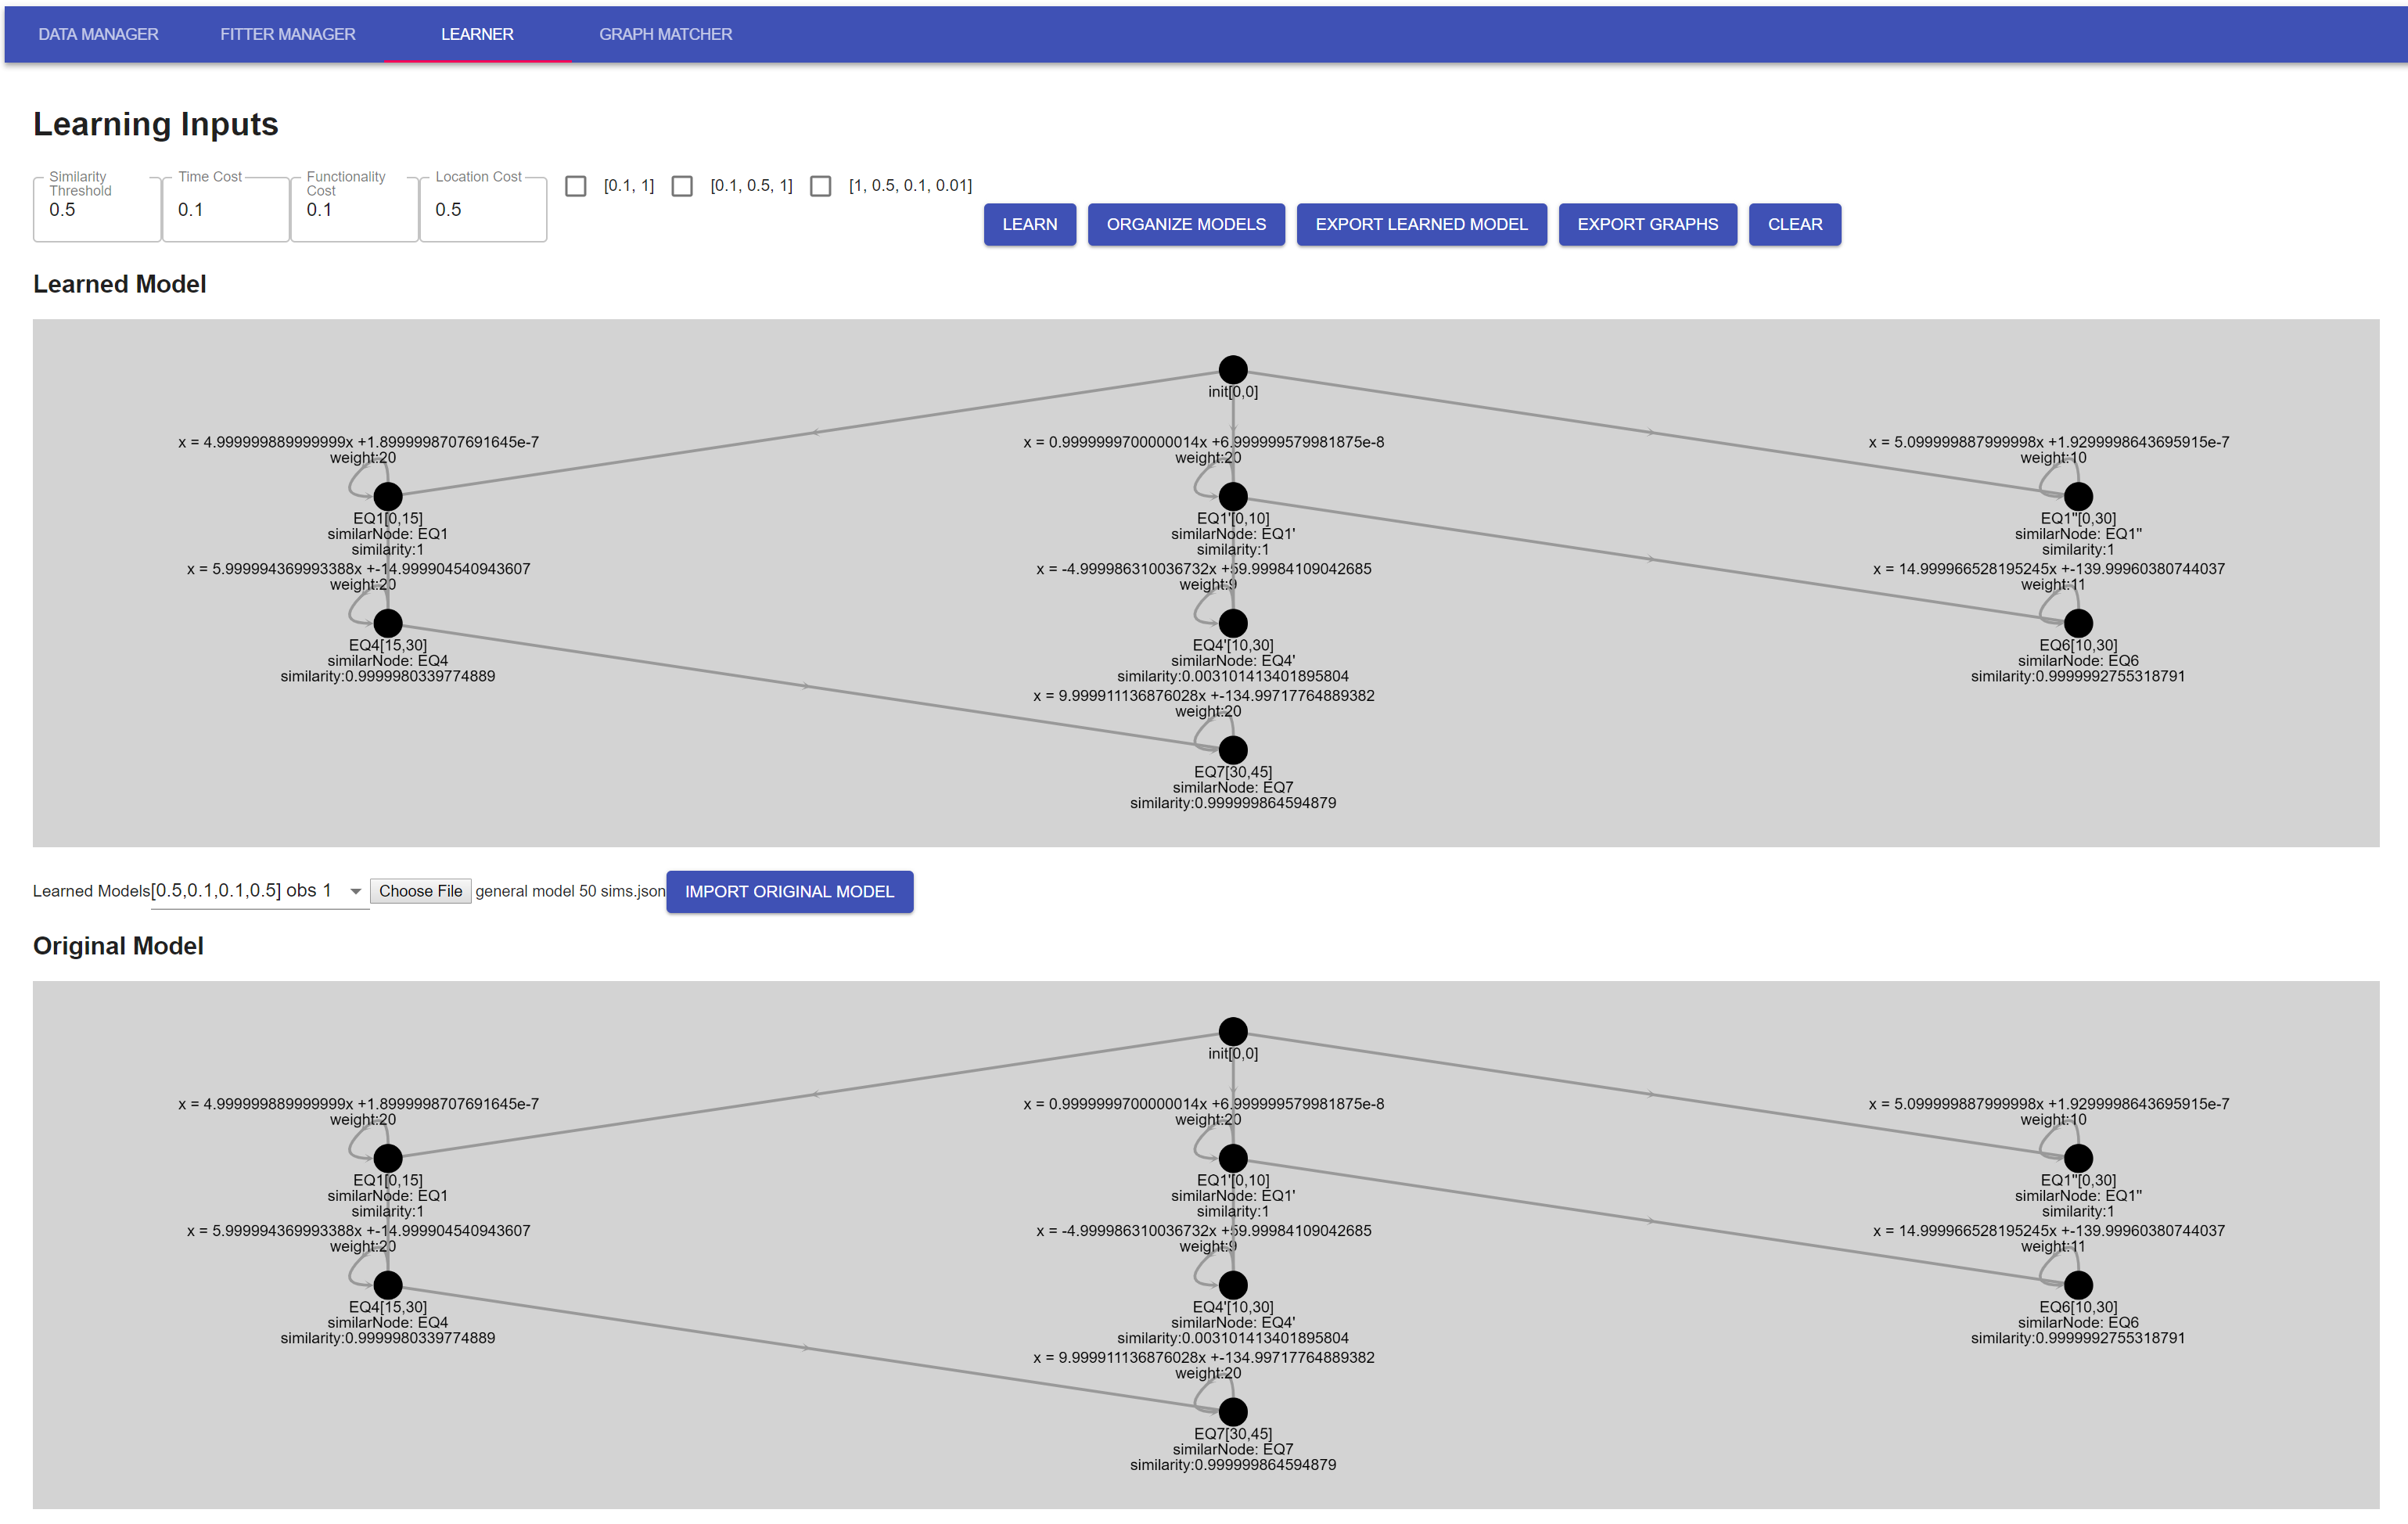
\includegraphics[scale=0.25]{./pictures/implementation/learning_manager.png}
	\caption{Implementation Learning Manager}
	\label{learning_manager}
\end{figure}

\newpage

\section{Graph Matcher}
The \texttt{Graph Matcher} component was created for visualizing how the matching of models is performed in incremental learning, whenever there exists an \textit{original model} (e.g. the imported model from \texttt{Learning Manager}) that can be compared against the \textit{learned model}. 
%
The similarity of the models is calculated by traversing both graphs simultaneously and matching the nodes, disregarding their labels and only by judging how close they are in terms of Euclidean distance. The user interface of the \texttt{Graph Matcher}, as seen in Figure \ref{graph_matcher} is essentially the same as the one from the \texttt{Learning Manager}, with an additional section called \textit{Matched Model}, where one can see which nodes from the learned model were matched with the ones from the original model. For simplicity and explanation purposes, we matched the two models from Figure \ref{learning_manager} and show the results in Figure \ref{graph_matcher_matched}. As seen in Figure \ref{graph_matcher_matched}, the learned model was successfully matched, as it is identical to the original model. The \textit{Graph Matcher} facilitates the interpretation of the comparison by coloring the edges and nodes in green when they were matched, and in red when they were not. Also, the \textit{Matched Model} section includes information of which node from the learned model was matched in the original model. The label \textit{lm} represents the name of the node of the learned model, and the label \textit{om} corresponds to the name of the node from the original model that was matched.
%
\begin{figure}[h]
	\centering
	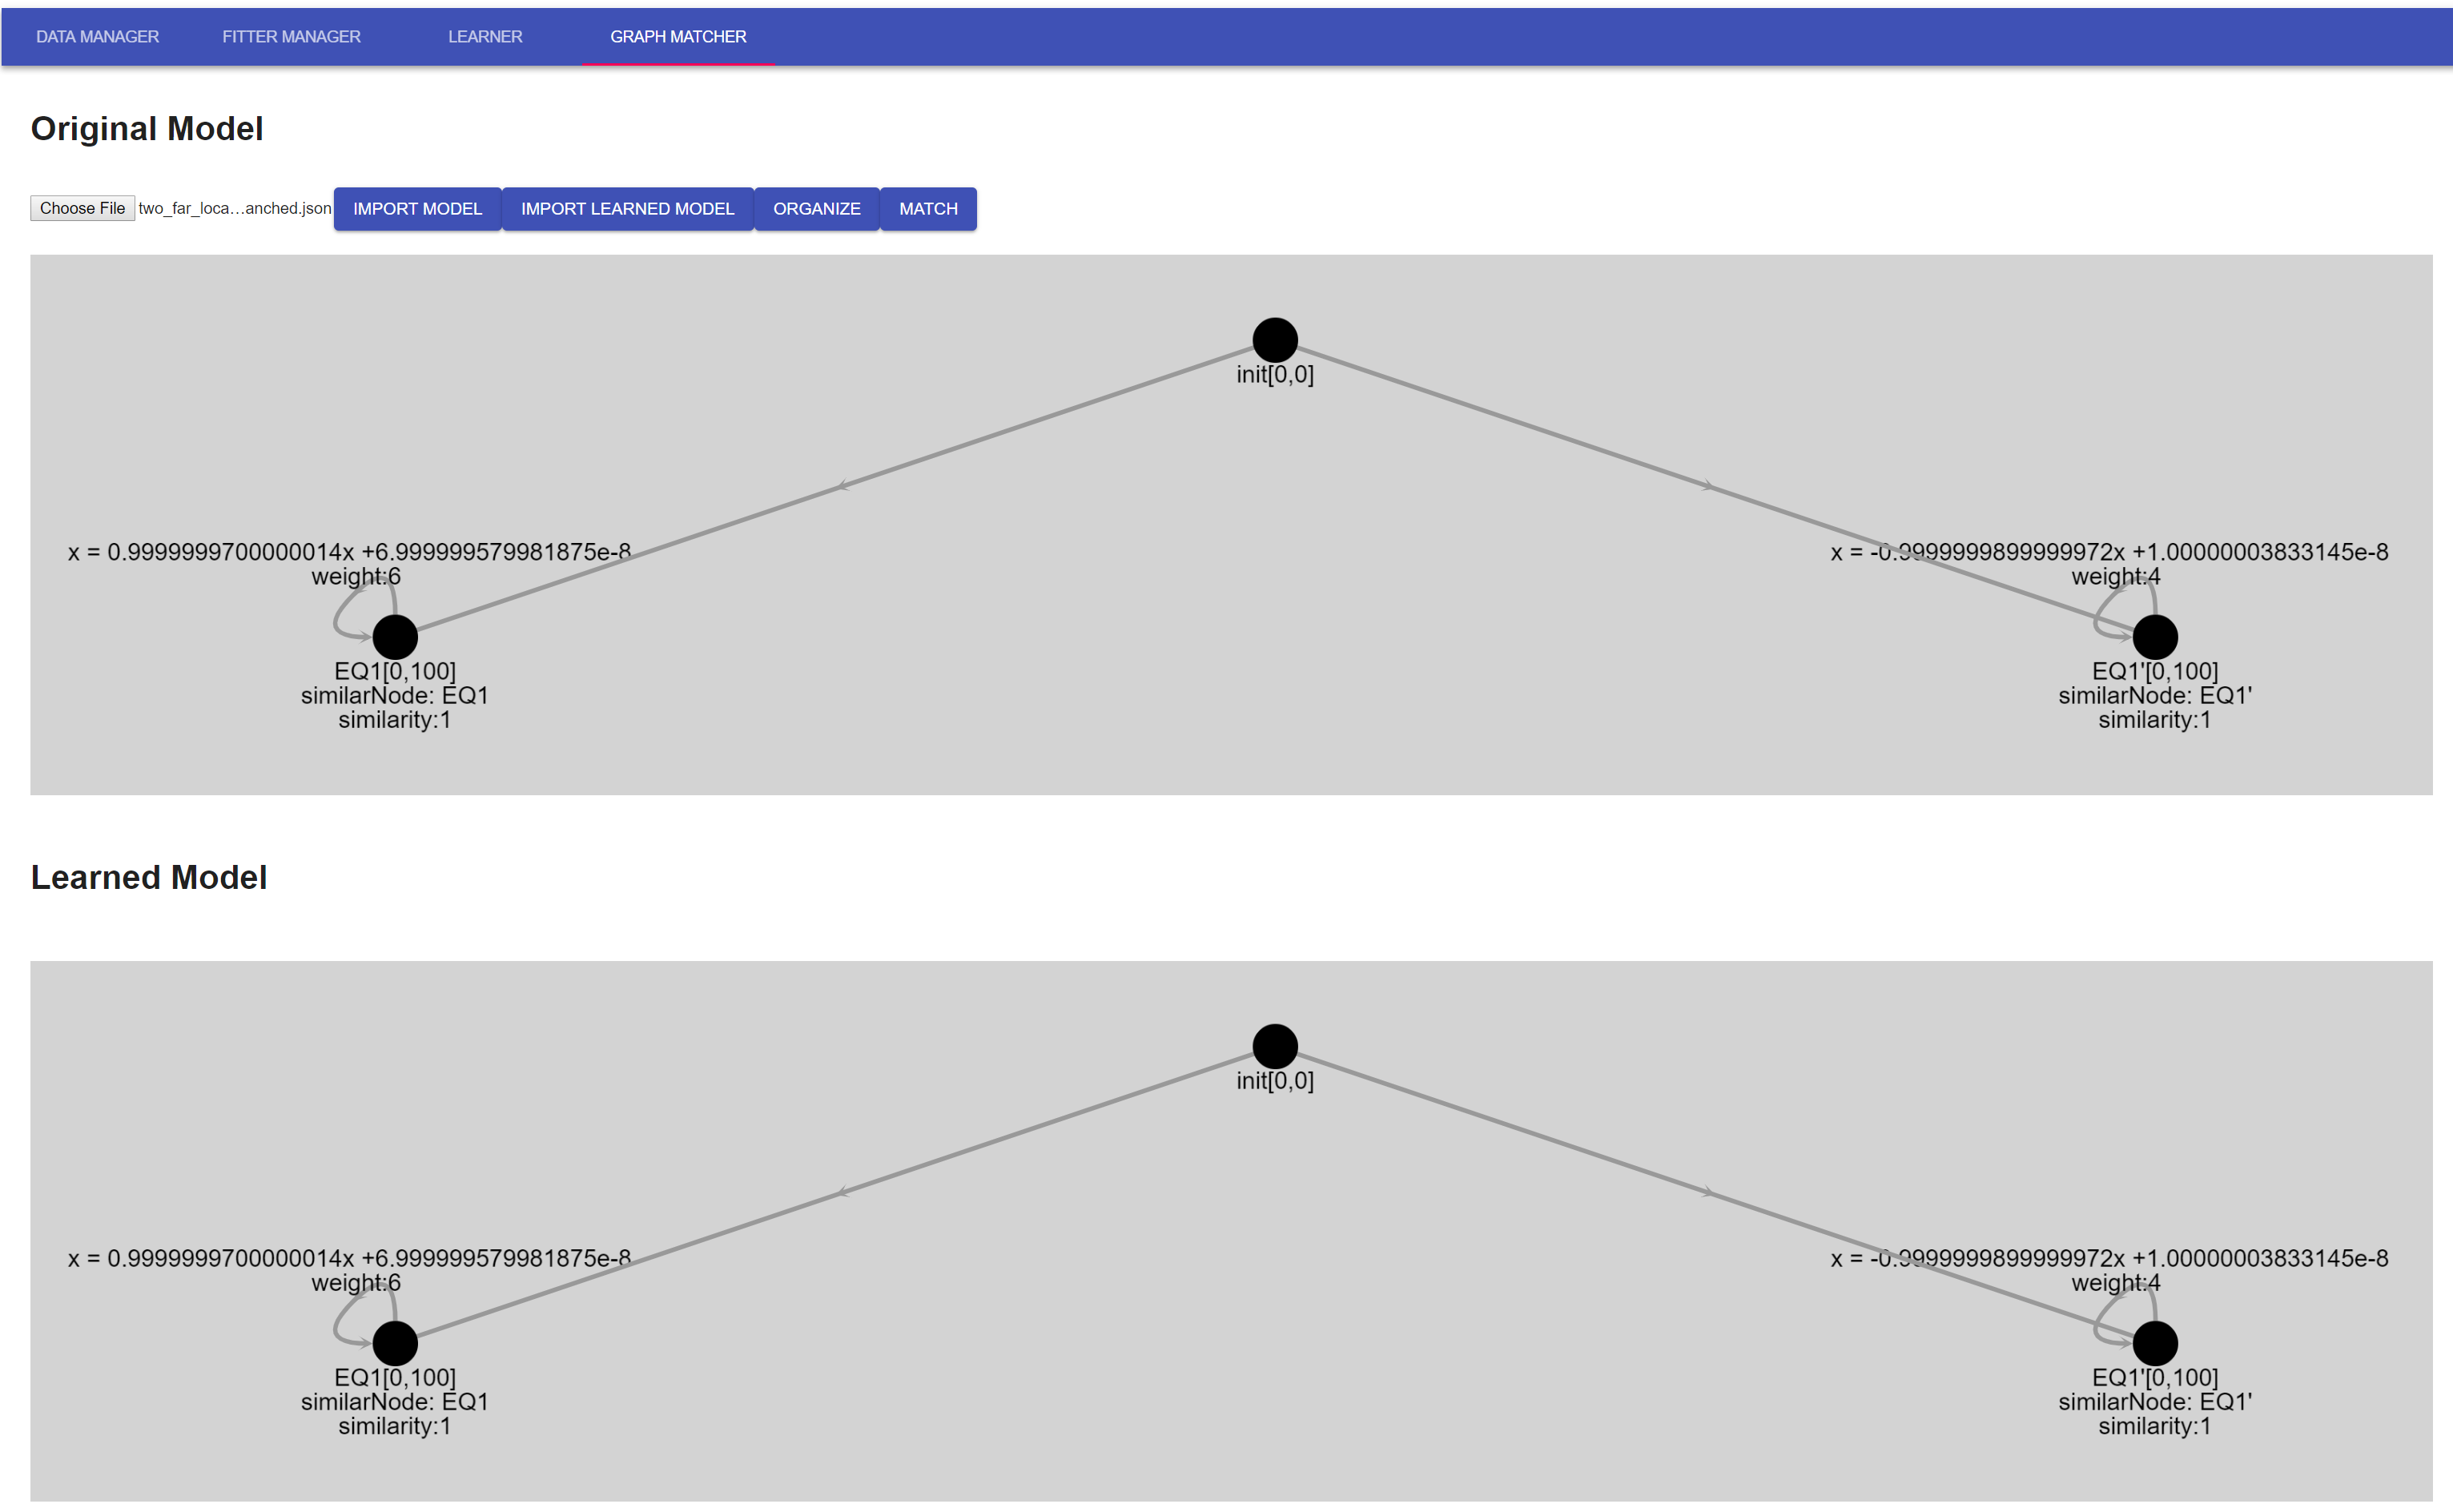
\includegraphics[scale=0.25]{./pictures/implementation/Graph_Matcher.png}
	\caption{Implementation Graph Matcher}
	\label{graph_matcher}
\end{figure}
\begin{figure}[h]
	\centering
	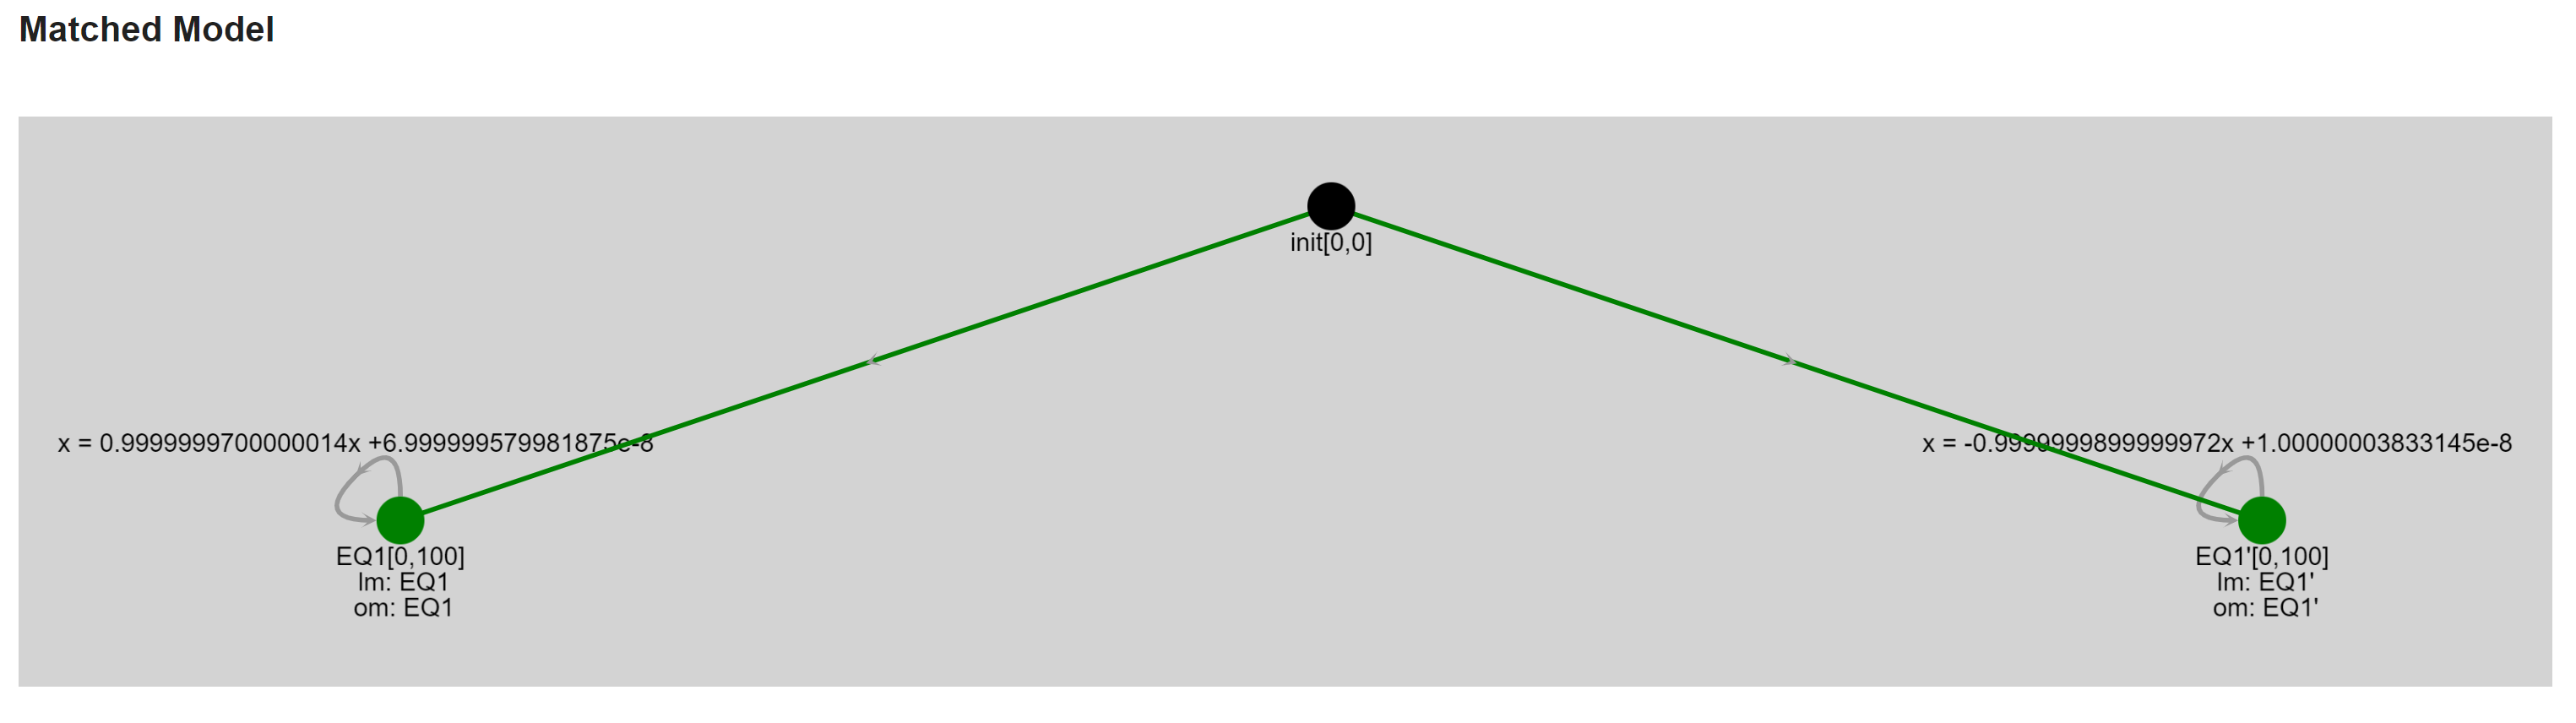
\includegraphics[scale=0.25]{./pictures/implementation/Graph_Matcher_1.png}
	\caption{Implementation Graph Matcher - Model matched section}
	\label{graph_matcher_matched}
\end{figure}




 
	
	\chapter{Experiments and Evaluation}	
	\label{chap:experimentation}
	In the following section we will demonstrate the impact that the values of the cost function parameters and the similarity threshold can have in the incremental learning approach.
%
%It is the case that we obtain different learned models depending on the combination of such values.\\ \\
%
Two sets of experiments were conducted. The first set consists of evaluating the impact of giving priority to one of the four possible parameters that we take into consideration in our approach, which are: \textit{similarity threshold}, \textit{time cost}, \textit{functionality cost} and \textit{location cost}. While the second set consists of finding optimal combinations of parameters that lead to good incremental learning. 
%
\section{Experiment 1} 
For the first type of experiment we concentrate on learning one model, depicted in Figure \ref{experiment_model_example}, and also referred as \textit{original model}. The model is categorized as complex for this project because it involves a mixture of branched and sequential nodes.
%
We focus in this section on evaluating how the incremental learning approach performs when a particular parameter is prioritized. For this, we simply set the prioritized parameter to the value of 1 and the others to the minimum allowed value of 0.1. We do not experiment with values of 0 because that would completely ignore some parameters of our approach, and it would also contradict the nature of this project, as each parameter has a role in the process. 
%There exists four possible parameters that are used for incremental learning, therefore, we performed a set of four sub-experiments to analyze the behavior of the learning process with respect to the prioritized parameters. 
%
\begin{figure}[h]
	\centering
	\makebox[\textwidth][c]{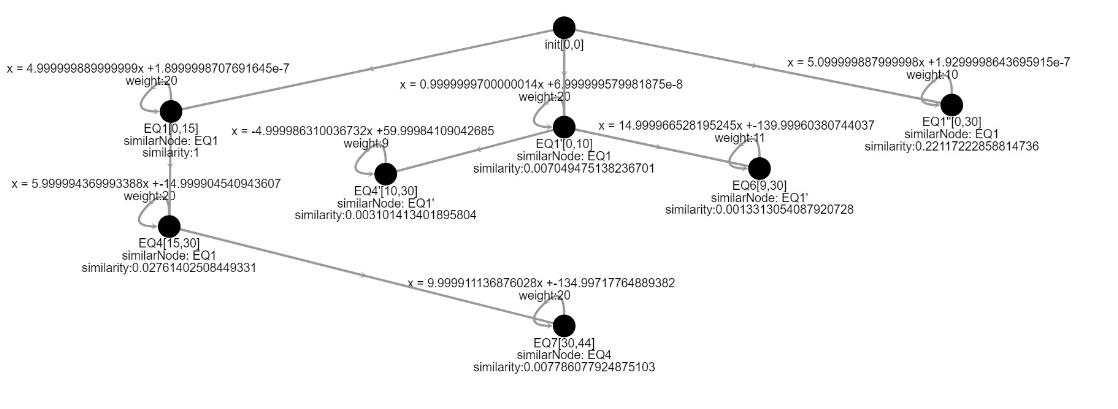
\includegraphics[width=1.0\textwidth]{./pictures/experiment.png}}%
	\caption{Experiment 1 Original Model}
	\label{experiment_model_example}
%	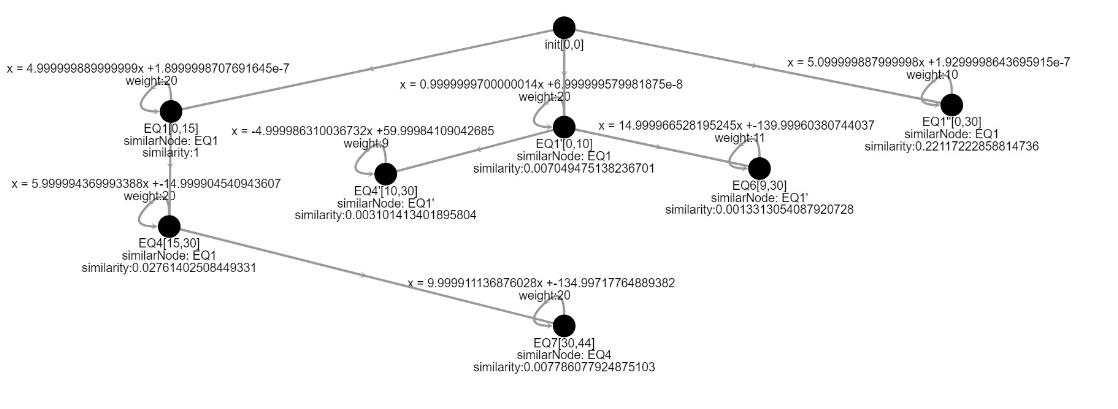
\includegraphics[scale=0.75]{./pictures/experiment.png}
\end{figure}

\subsection{Sub-Experiment 1 - Similarity Prioritized}
The \textit{Similarity threshold} is responsible for discriminating which learned nodes are close enough to be merged in the learning progress. In this experiment, its value is increased to 1, meaning that only completely identical locations will be considered in the evaluation of merging nodes via the cost function of our approach. 

\subsubsection{Results}
%We can see in Figure \ref{experiment_similarity_threshold} the structure of the final learned model. 
Despite the difference between the original model and the learned model from Figure \ref{experiment_similarity_threshold}, one can notice that the learned model actually contains the structure of the original one, but with additional nodes. 
\begin{figure}[h]
	\centering
	\includegraphics[scale=0.4]{./pictures/similarity_experiment/learnedModel.png}
	\caption{Sub-Experiment 1 - Similarity Prioritized - Learned Model}
	\label{experiment_similarity_threshold}
\end{figure}

\subsubsection{Evaluation}
The nature of this experiment can be explained by analyzing two particular learned models. The learned model from Figure \ref{experiment_similarity_threshold_1} represents the best performance of the learning approach, as all of the observations until that point were completely identical (e.g. Figure \ref{experiment_similarity_threshold_sim} in observation 10).
%
It is not until we see a slightly different observation, that the learned model begins to add redundant locations due to the strict criteria of the similarity threshold. One can see that the last two nodes (from left to right) of Figure \ref{experiment_similarity_threshold_2} are identical in terms of functionality, but were discovered in slightly different time ranges. Node \textit{EQ4"} was discovered in the time range of 10-30, while the other next to it was discovered in the range of 9-10. This minimal difference in time constraints is detected by the learner and therefore a new node is added, to not loose precision of the observed data.
%
Also being the reason that the replacement cost from Figure \ref{experiment_similarity_threshold_rep} always stays in 0, because we are only replacing identical locations, according to the similarity threshold of 1. Whenever there is a slight difference in the learned observations, a new node will be added. Therefore, one can see in Figure \ref{experiment_similarity_threshold_costs} that peaks, represent each node that was added to the learned model. It is also important to notice that from observation 43 until the end of the simulation (e.g. observation 100) the graph similarity stays constant because there are no new observations at any point. 
%
\newpage

\begin{figure}[h]
	\centering
	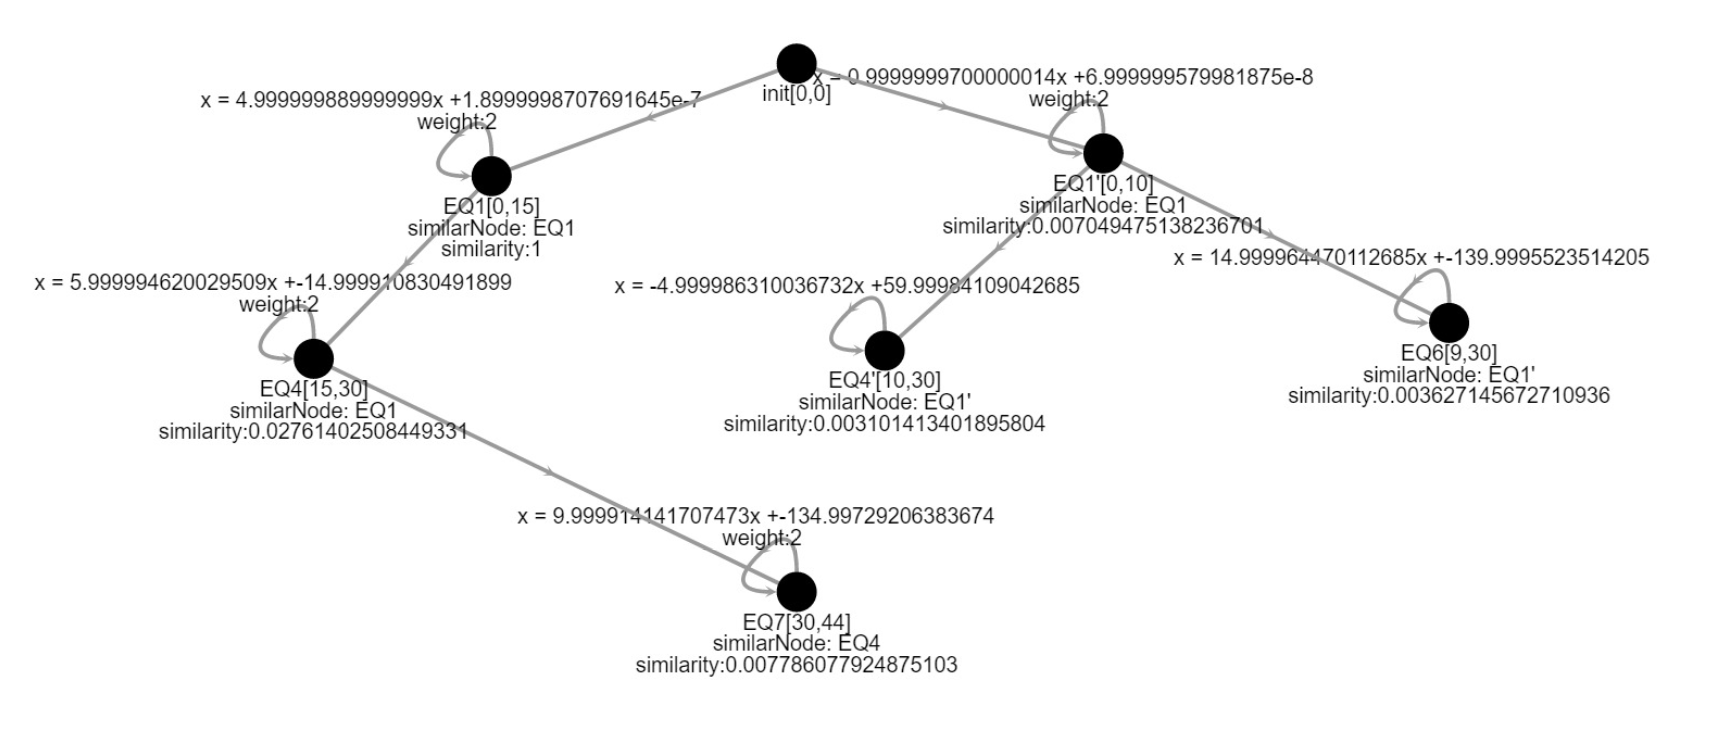
\includegraphics[scale=0.38]{./pictures/similarity_experiment/learnedModel_Obs10.png}
	\caption{Sub-Experiment 1 - Similarity Prioritized - Learned Model - Observation 10}
	\label{experiment_similarity_threshold_1}
\end{figure}

\begin{figure}[h]
	\centering
	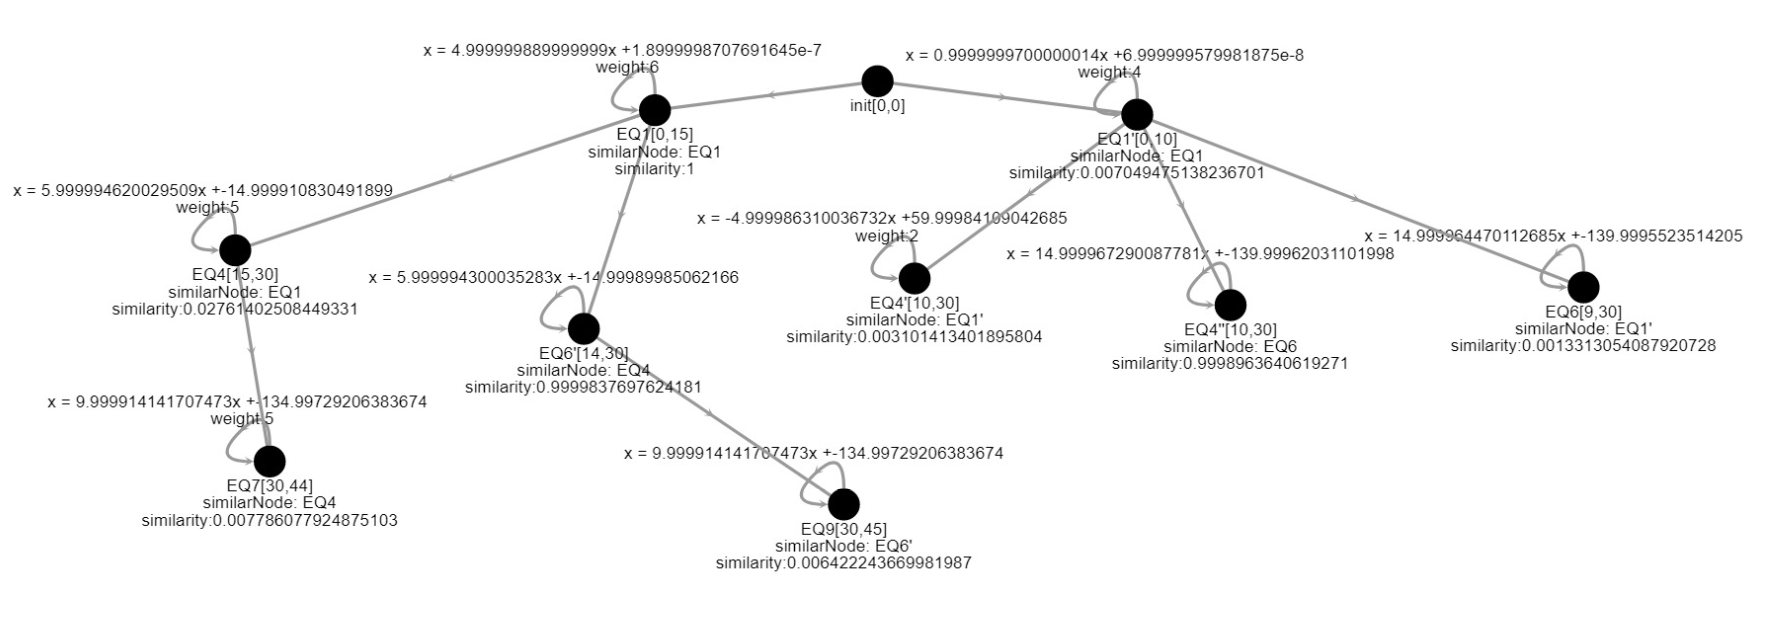
\includegraphics[scale=0.38]{./pictures/similarity_experiment/learnedModel_Obs26.png}
	\caption{Sub-Experiment 1 - Similarity Prioritized - Learned Model - Observation 26}
	\label{experiment_similarity_threshold_2}
\end{figure}

\newpage

\begin{figure}[h]
	\centering
	\includegraphics[scale=0.7]{./pictures/similarity_experiment/similarity.png}
	\caption{Sub-Experiment 1 - Similarity Prioritized - Graph Similarity}
	\label{experiment_similarity_threshold_sim}
\end{figure}

\newpage

\begin{figure}[h]
	\centering
	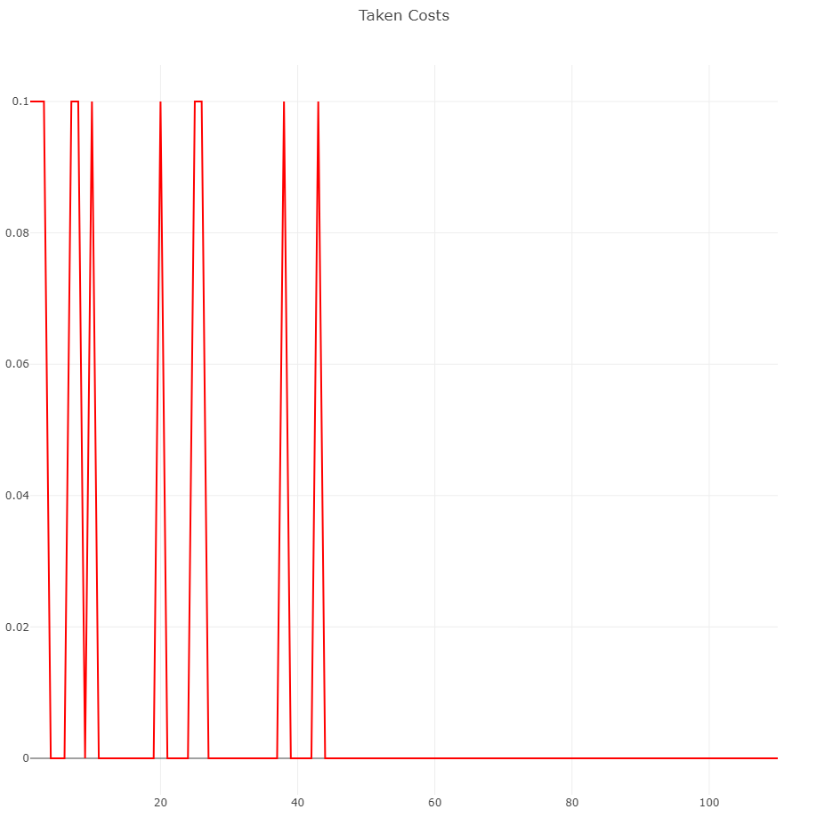
\includegraphics[scale=0.7]{./pictures/similarity_experiment/costs.png}
	\caption{Sub-Experiment 1 - Similarity Prioritized - Taken Costs}
	\label{experiment_similarity_threshold_costs}
\end{figure}

\begin{figure}[h]
	\centering
	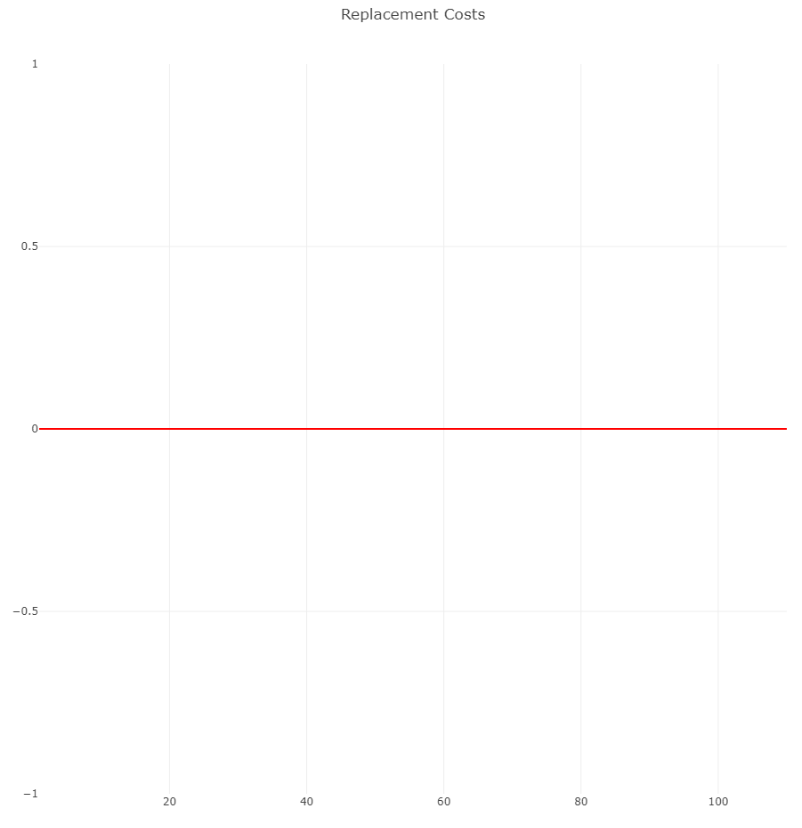
\includegraphics[scale=0.7]{./pictures/similarity_experiment/replacement.png}
	\caption{Sub-Experiment 1 - Similarity Prioritized - Replacement Costs}
	\label{experiment_similarity_threshold_rep}
\end{figure}

\newpage

\subsection{Sub-Experiment 2 - Time and Functionality Prioritized}
For this experiment the \textit{Time Cost} and \textit{Functionality Cost} will be set to 1 simultaneously. This is because the cost function explained in \Cref{chap:incremental_Learning}, calculates the error propagation of nodes based on the difference of time constraints and functionality among other nodes and incoming observations. Therefore, it is not meaningful to ignore one of the two criteria while evaluating observations. 

\subsubsection{Results}
In Figure \ref{time_func_experiment} we can see the final learned model. It is very interesting and also meaningful to notice that the structure resembles the one from the previous experiment in Figure \ref{experiment_similarity_threshold}. This is to be expected with the selected parameters, as the nodes must be almost identical when merging. Meaning that minimal differences in terms of functionality or time constraints will have a high cost, and will therefore lead to the addition of new nodes.

\begin{figure}[h]
	\centering
	\makebox[\textwidth][c]{\includegraphics[width=1.0\textwidth]{./pictures/time_functionality_experiment/learnedModel.png}}%
	\caption{Sub-Experiment 2 - Time and Functionality Prioritized - Learned Model}
	\label{time_func_experiment}
%	\includegraphics[scale=0.4]{./pictures/time_functionality_experiment/learnedModel.png}
\end{figure}

\subsubsection{Evaluation}
Despite the fact that we obtained the same learned model as in the previous experiment, the observations that caused the evolution of the model were not the same. Let us take a look at the peaks of the replacement costs from Figure \ref{time_func_experiment_rep}. Each peak represents an added location, as it is always the case that the cost of replacing a location surpasses the cost of adding one, due to the difference of time constraints and functionalities of nodes.
%
We can see in Figure \ref{time_func_experiment_sim_1} that the so far learned model contains an extra location on the bottom-right corner (e.g. node labeled as EQ6), causing the similarity to stay in 0.85 (as seen in Figure \ref{time_func_experiment_sim}), as the extra node could not be matched in the original model. In this particular case, the functionality cost did not play a role because node \textit{EQ4"} and \textit{EQ6} were identical in terms of functionality and only differed in time constraints by 1 time unit (same case as in the previous sub-experiment), causing the learner to add a new node to retain precision of the observations. \\ \\
%
Let us now pay attention to the highest peak from the graph shown in Figure \ref{time_func_experiment_rep}, as it represents the most expensive change that happened in the simulation. The reason of this peak is strongly related to the low value of the \textit{similarity threshold} (e.g. 0.1). 
%
In observation 38, a merge between node \textit{EQ1} and node \textit{EQ1"} (the opposite nodes of the first \textit{depth-level} of the graph) from the model shown in Figure \ref{time_func_experiment_sim_2} was attempted. 
%
This happened because the similarity of both nodes is 0.22 (number obtained by Algorithm \ref{measureDistances}), thus similar enough to be merged according the the similarity threshold value of 0.1.
%
Nevertheless, the merge was unsuccessful because there also existed difference in the time constraints. One node was observed in the range of 0-15 time units and the other one in the range of 0-30 time units. This accumulated a high cost of merging the two nodes because of their different time constraints. 
%
For this case, the functionality cost already showed a high cost that would have forced the learner to add a new node, but the difference in time constraints was also taken into account, causing the final cost to be very high. 
%
In the end, we could not perfectly learn the observed model mainly because of the strict parameters that were utilized while trying to merge similar nodes. The learned model is still adding redundant nodes of similar observations when they are not almost identical, as seen in each peak from Figure \ref{time_func_experiment_costs}. 
%
%
\begin{figure}[h]
	\centering
	\makebox[\textwidth][c]{\includegraphics[width=1.0\textwidth]{./pictures/time_functionality_experiment/learnedModel_Obs20.png}}%
	\caption{Sub-Experiment 2 - Time and Functionality Prioritized - Learned Model - Observation 20}
	\label{time_func_experiment_sim_1}
%	\includegraphics[scale=0.4]{./pictures/time_functionality_experiment/learnedModel_Obs20.png}
\end{figure}
%
\begin{figure}[h]
	\centering
	\makebox[\textwidth][c]{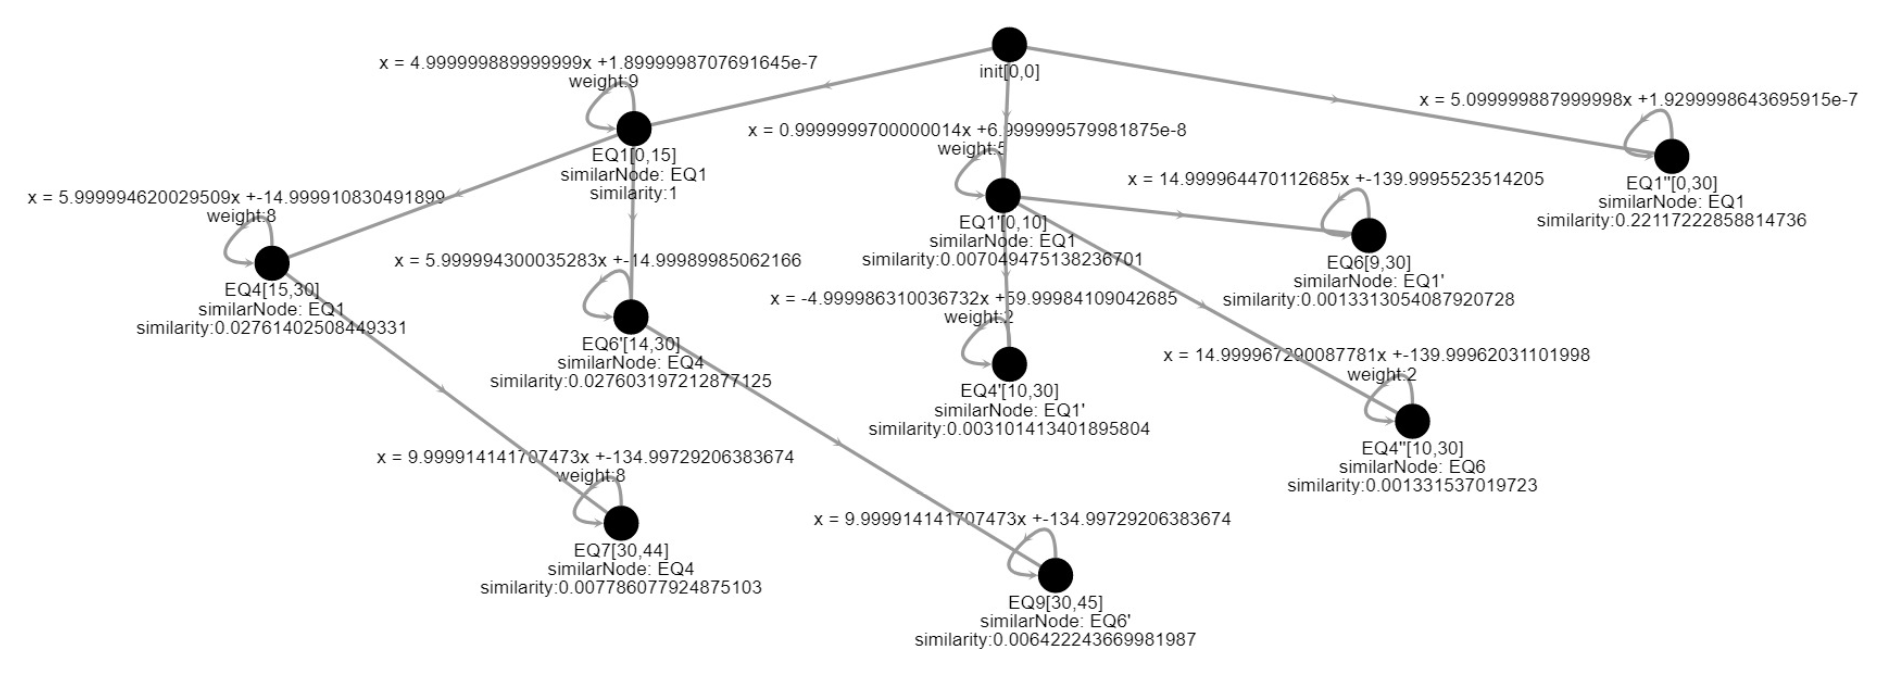
\includegraphics[width=1.0\textwidth]{./pictures/time_functionality_experiment/learnedModel_Obs38.png}}%
	\caption{Sub-Experiment 2 - Time and Functionality Prioritized - Learned Model - Observation 38}
	\label{time_func_experiment_sim_2}
%	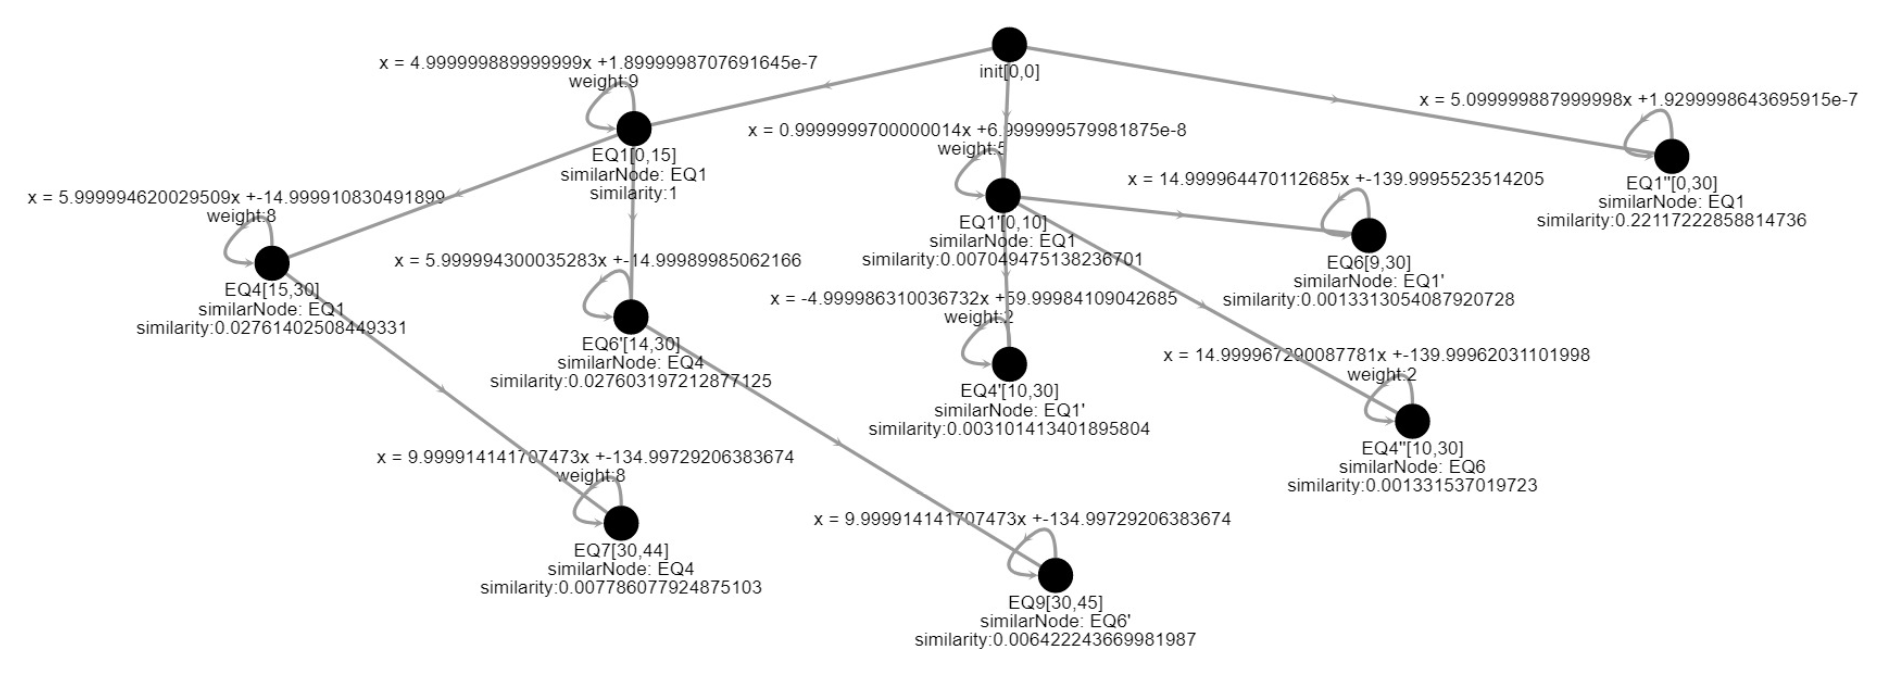
\includegraphics[scale=0.4]{./pictures/time_functionality_experiment/learnedModel_Obs38.png}
\end{figure}
%
\newpage

\begin{figure}[h]
	\centering
	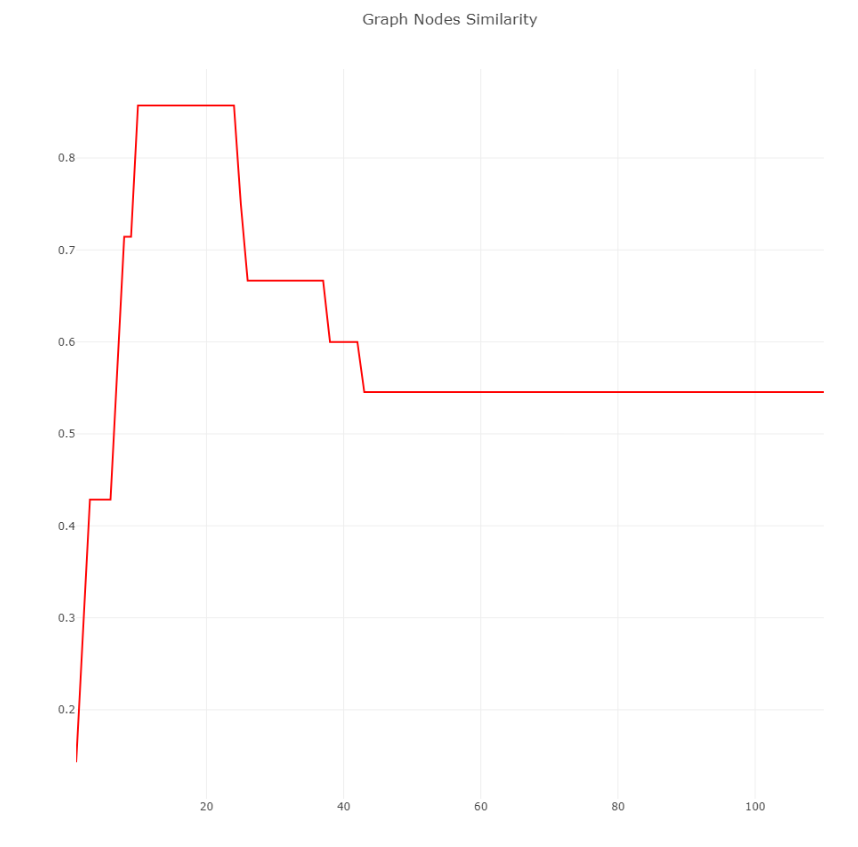
\includegraphics[scale=0.7]{./pictures/time_functionality_experiment/similarity.png}
	\caption{Sub-Experiment 2 - Time and Functionality Prioritized - Graph Similarity}
	\label{time_func_experiment_sim}
\end{figure}
%
\newpage
%
\begin{figure}[h]
	\centering
	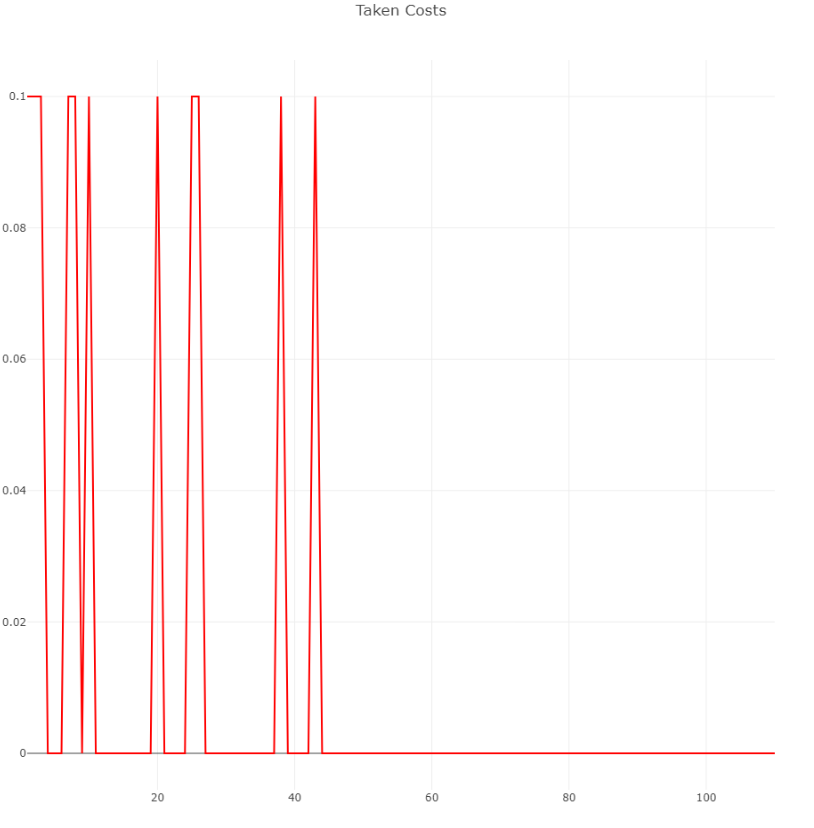
\includegraphics[scale=0.5]{./pictures/time_functionality_experiment/costs.png}
	\caption{Sub-Experiment 2 - Time and Functionality Prioritized - Taken Costs}
	\label{time_func_experiment_costs}
\end{figure}
%
\newpage
%
\begin{figure}[h]
	\centering
	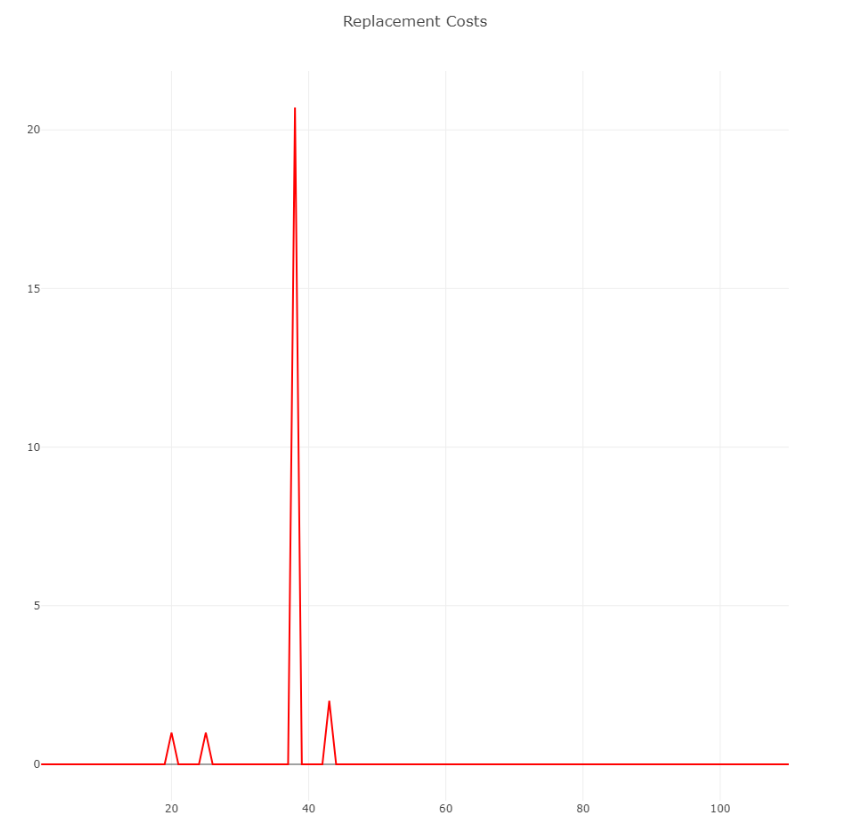
\includegraphics[scale=0.5]{./pictures/time_functionality_experiment/replacement.png}
	\caption{Sub-Experiment 2 - Time and Functionality Prioritized - Replacement Costs}
	\label{time_func_experiment_rep}
\end{figure}

\subsection{Sub-Experiment 3 - Node Addition Prioritized}
In this final experiment we set a high cost for adding locations (e.g. 1.0), while the other parameters are set to a low value (e.g. 0.1). Meaning that the learned model will be able to merge slight changes or noise from observations without needing to add an extra node every time that a different observation is learned. 

\subsubsection{Results}
As seen in Figure \ref{addition_experiment}, the learned model completely matches the original one. It was the case in this experiment because the learning process gave more priority (or cost) to the addition of new nodes. Which means that nodes that were added in the learned model were very distinguished among others in terms of time constraints and functionality, while similar nodes and observations were merged. 

\begin{figure}[h]
	\centering
	\makebox[\textwidth][c]{\includegraphics[width=1.0\textwidth]{./pictures/addition_experiment/learnedModel.png}}%
	\caption{Sub-Experiment 3 - Node Addition Prioritized - Learned Model}
	\label{addition_experiment}
%	\includegraphics[scale=0.4]{./pictures/addition_experiment/learnedModel.png}
\end{figure}

\subsubsection{Evaluation}
As we know that the original model was successfully learned, we will explain in detail why that was the reason by interpreting two particular observations that made the difference in the learning process. Looking at the first peak of Figure \ref{addition_experiment_rep}, the observation number 20 perfectly matched the functionality of node \textit{EQ6} (node located at the medium-right corner of Figure \ref{addition_experiment_sim_1}), with the only difference of 1 time unit from the observed time constraints. In the previous experiments, this difference of time would have caused the learning process to add an extra node to express the observation. 
%
But for this experiment it is not the case, as the cost of merging minimal time constraints and functionalities of nodes is very low. Therefore, despite the minimal difference in time constraints, the learned model ignores the unseen time unit to keep a minimal number of nodes, but it also sacrifices some precision of the information learned.
%
Although, if we take a look at the highest peak of the previous graph, one can easily see that the cost of replacing a node is higher than the one of adding a new one. The reason of this high cost is because a new observation was discovered in that point (e.g. the top-right node \textit{EQ1"} from Figure \ref{addition_experiment}). This last added node could not be merged with the closest node found (node \textit{EQ1} located at the top-left corner from the same figure) mainly due to their differences in terms of functionality and time constraints. The functionality differed by 0.2 (e.g. Euclidean distance calculated by Algorithm \ref{measureDistances}) and the number of unseen times were 15 (as in the sub-experiment 2). Given the flexibility of the learned to merge similar nodes, this difference was considered great enough to discard the merging procedure and to add the observation as a new node. At this point, it is important to remark that if the nodes were to be merged, we could have had fewer locations in our learned model and less precision in the data. But this change would have caused the similarity of our models to decrease significantly.
%
%in this case, it also did not succeed to do so because the difference in functionality and time constraints was high enough to express th observation as a new node. Otherwise the merge of the nodes would have propagated significant errors to the learned model. 
%
Consequently, one can see in Figure \ref{addition_experiment_costs} that the cost of adding a node (e.g. 1.0) was taken instead of the one of merging nodes (e.g. 2.0). And it is indeed from this point the no new significant behavior was learned from the observations, as the similarity between the original model and the learned model remained optimal and constant, as depicted in Figure \ref{addition_experiment_sim}
%
\newpage

\begin{figure}[h]
	\centering
	\includegraphics[scale=0.4]{./pictures/addition_experiment/learnedModel_Obs20.png}
	\caption{Sub-Experiment 3 - Node Addition Prioritized - Learned Model - Observation 20}
	\label{addition_experiment_sim_1}
\end{figure}

\newpage

%%
%\begin{figure}[h]
%	\centering
%	\caption{Sub-Experiment 1 - Similarity Prioritized - Learned Model - Observation 38}
%	\label{time_func_experiment_sim_2}
%	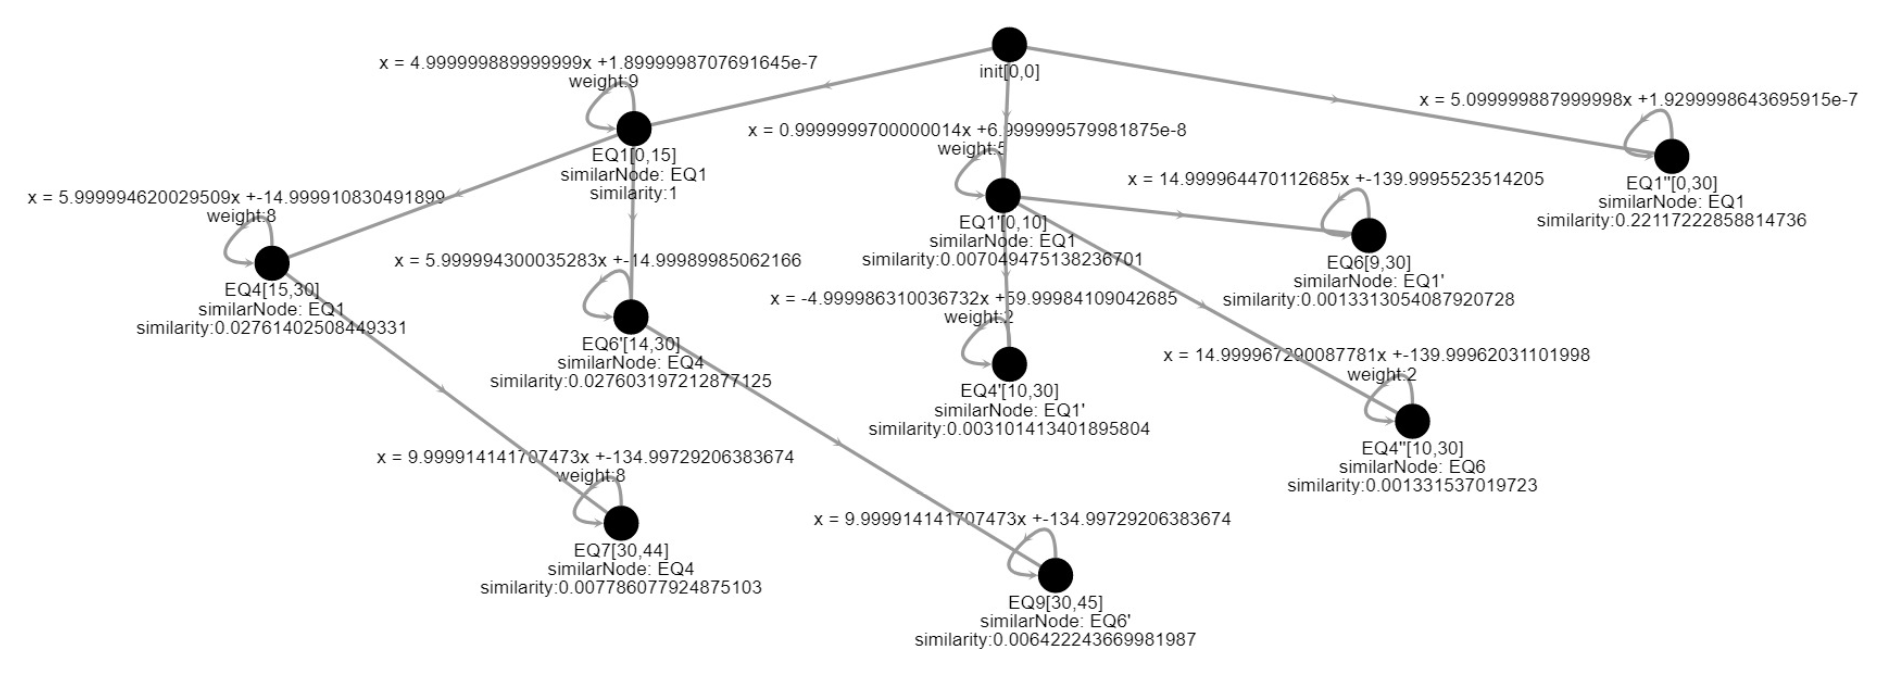
\includegraphics[scale=0.4]{./pictures/time_functionality_experiment/learnedModel_Obs38.png}
%\end{figure}
%%
\begin{figure}[h]
	\centering
	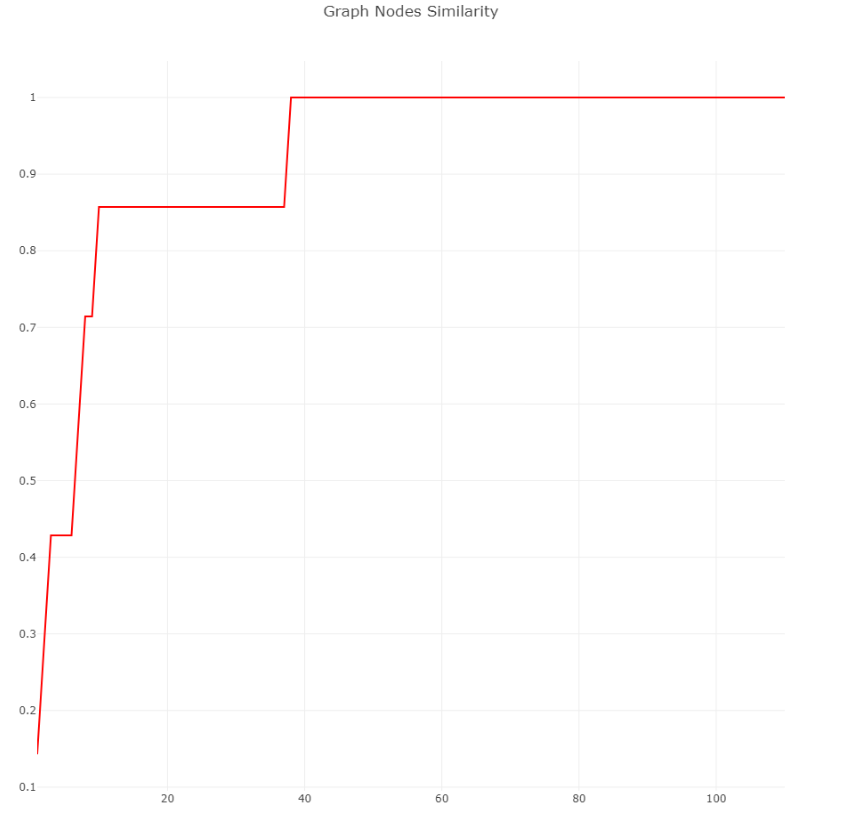
\includegraphics[scale=0.7]{./pictures/addition_experiment/similarity.png}
	\caption{Sub-Experiment 3 - Node Addition Prioritized - Graph Similarity}
	\label{addition_experiment_sim}
\end{figure}
%
\newpage

\begin{figure}[h]
	\centering
	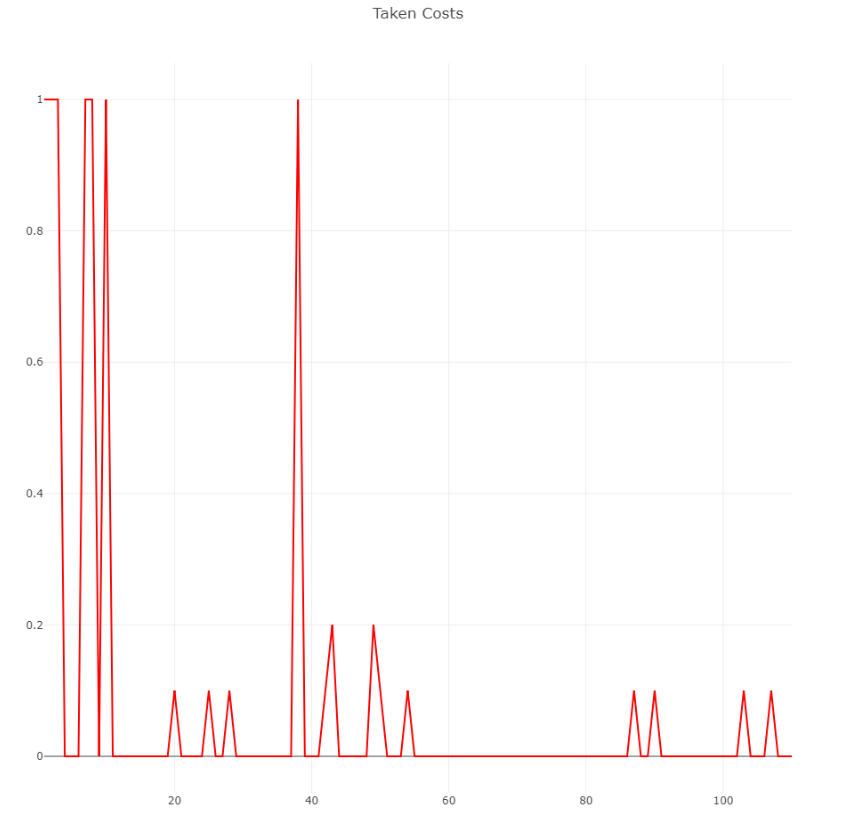
\includegraphics[scale=0.5]{./pictures/addition_experiment/costs.png}
	\caption{Sub-Experiment 3 - Node Addition Prioritized - Taken Costs}
	\label{addition_experiment_costs}
\end{figure}
%
\begin{figure}[h]
	\centering
	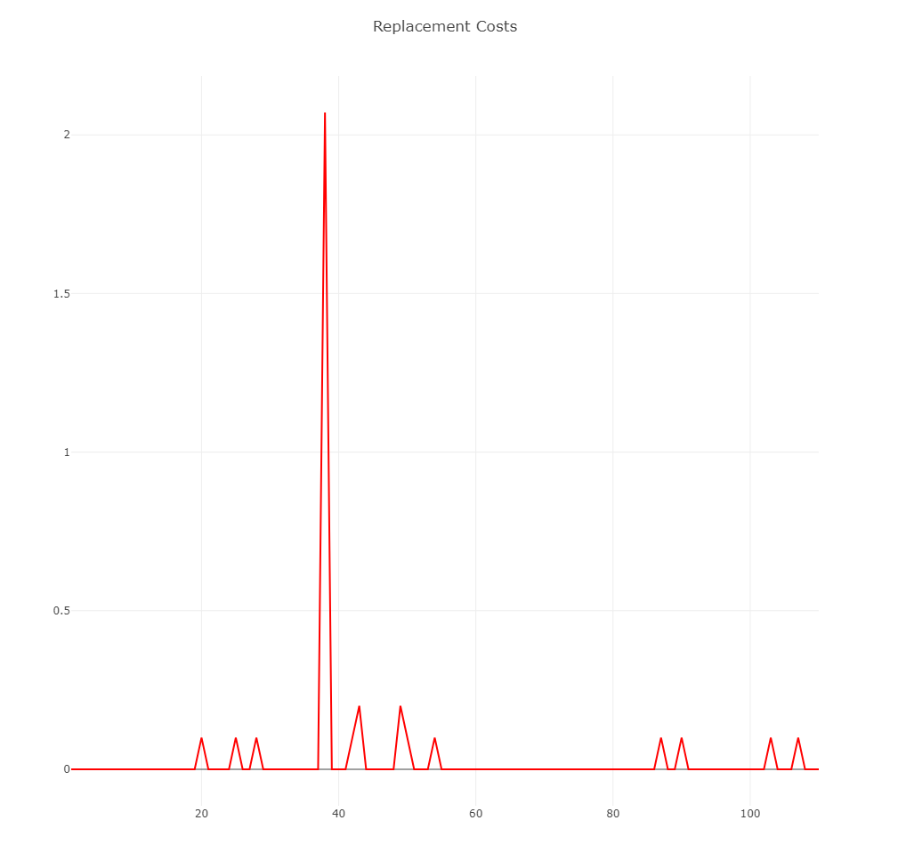
\includegraphics[scale=0.5]{./pictures/addition_experiment/replacement.png}
	\caption{Sub-Experiment 3 - Node Addition Prioritized - Replacement Costs}
	\label{addition_experiment_rep}
\end{figure}

\newpage

\section{Experiment 2}
After observing how the incremental learning process behaves differently given prioritized parameters, in this section we attempt to find the optimal combination of parameters in which an observed model can be learned. In the previous experiment, we restricted ourselves to one type of combination and to two possible values (e.g. 0.1 and 1) for the \textit{cost parameters} and \textit{similarity threshold}. In this experiment we restrict ourselves to three different values: 0.1, 0.5, and 1, but with the possibility of allowing different combinations of them while learning observations. Therefore, we divided this section into two sub-experiments. In the first sub-experiment we learn a model with combinations of branches and sequential nodes. Whereas in the second sub-experiment we learn two simple and relatively small models. The purpose of this division is to demonstrate how the learning process behaves with different types of models.

\subsection{Sub-Experiment 1}
We used the same model as in Experiment 1 (e.g. Given in Figure \ref{experiment_model_example}), and learned it once again by using 81 combinations of different parameters for the \textit{cost function} and the \textit{similarity threshold}.

\subsubsection{Results}
At the end, 63 combinations could match 54\% of the original model (learned model in Figure \ref{combination_experiment_1}), 6 out of 81 matched 70\% of original model (learned model in Figure \ref{combination_experiment_2}), and only 12 combinations could match it by 100\%. 
% 
\begin{figure}[h]
	\centering
	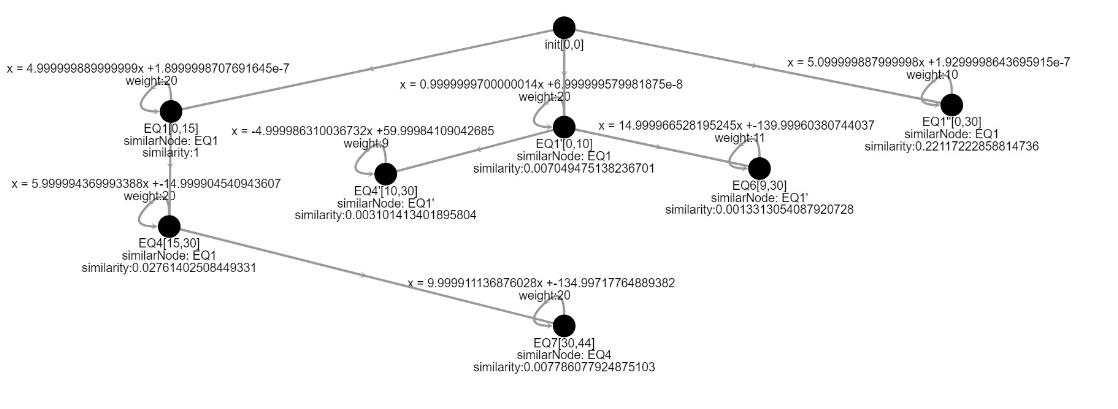
\includegraphics[scale=0.6]{./pictures/experiment.png}
	\caption{Sub-Experiment 1 - Original Model}
	\label{combination_experiment_model}
\end{figure}

\begin{figure}[h]
	\centering
	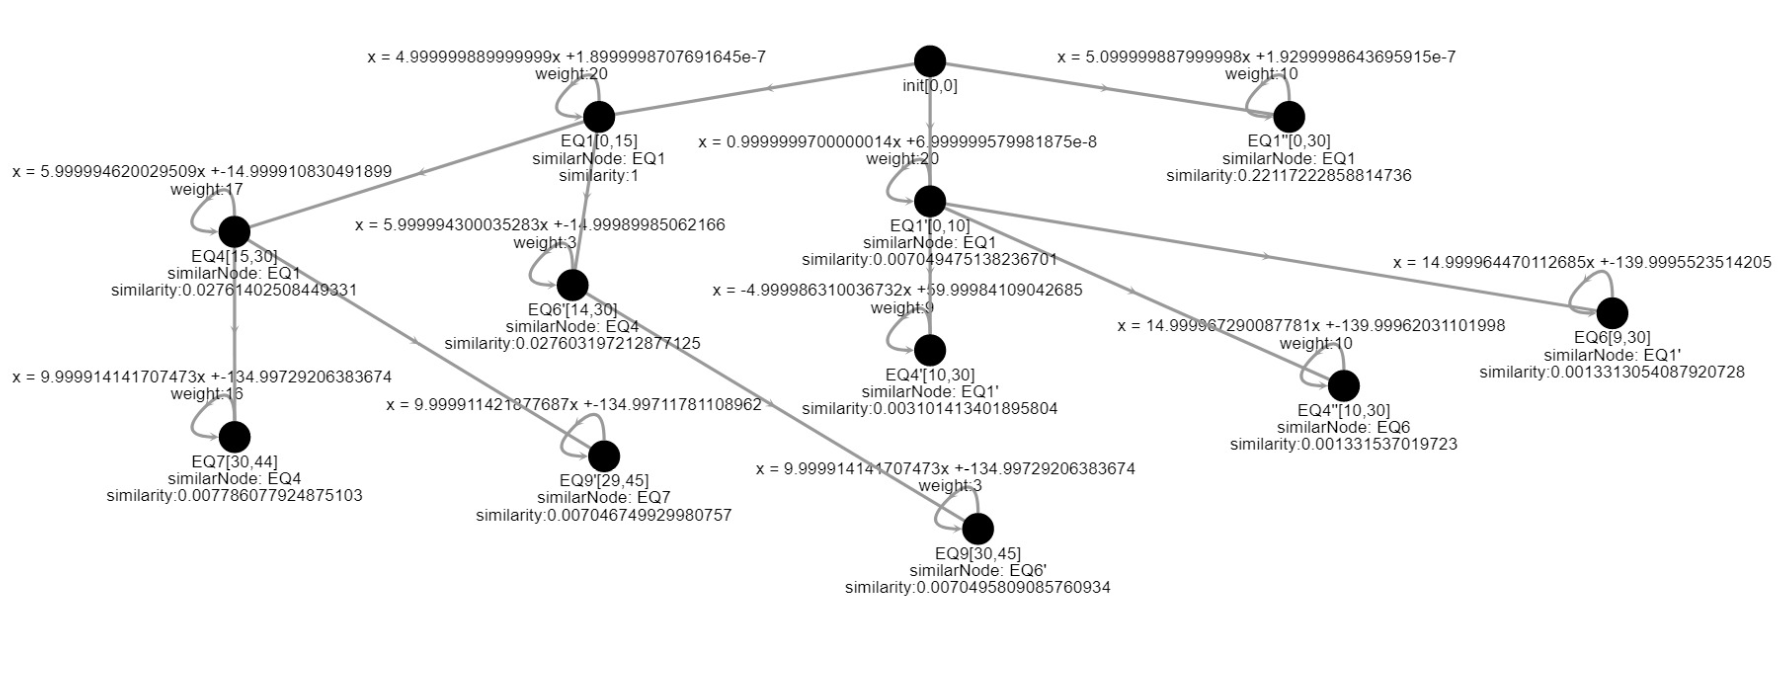
\includegraphics[scale=0.4]{./pictures/combination_experiment/learnedModel_worse.png}
	\caption{Sub-Experiment 1 - 54\% of original mode learned}
	\label{combination_experiment_1}
\end{figure}

\begin{figure}[h]
	\centering
	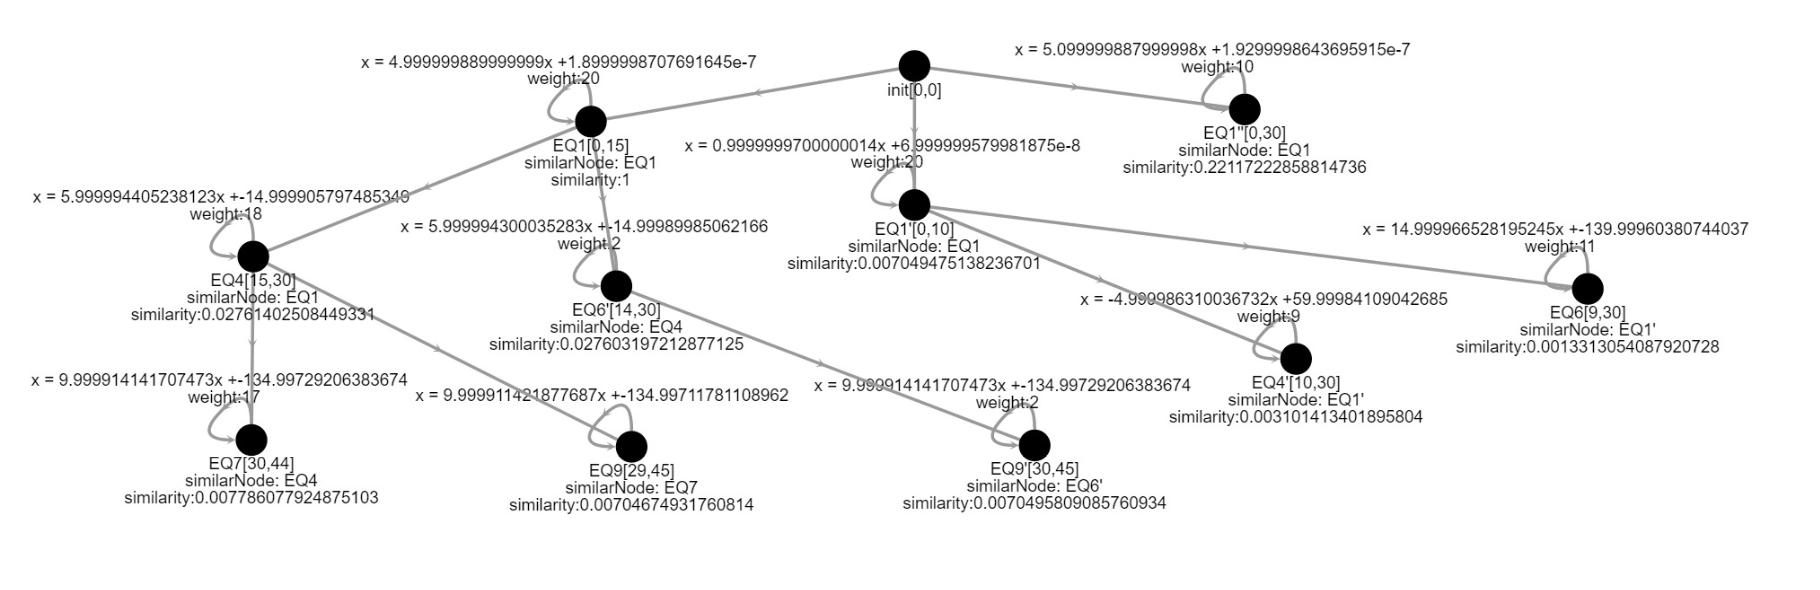
\includegraphics[scale=0.4]{./pictures/combination_experiment/learnedModel_better.png}
	\caption{Sub-Experiment 1 - 70\% of original mode learned}
	\label{combination_experiment_2}
\end{figure}

%\begin{figure}[h]
%	\centering
%	\caption{Experiment 2 - Graph Similarities}
%	\label{addition_experiment_costs}
%	\includegraphics[scale=0.5]{./pictures/combination_experiment/similarity.png}
%\end{figure}
%%
%\begin{figure}[h]
%	\centering
%	\caption{Experiment 2  - Replacement Costs}
%	\label{addition_experiment_rep}
%	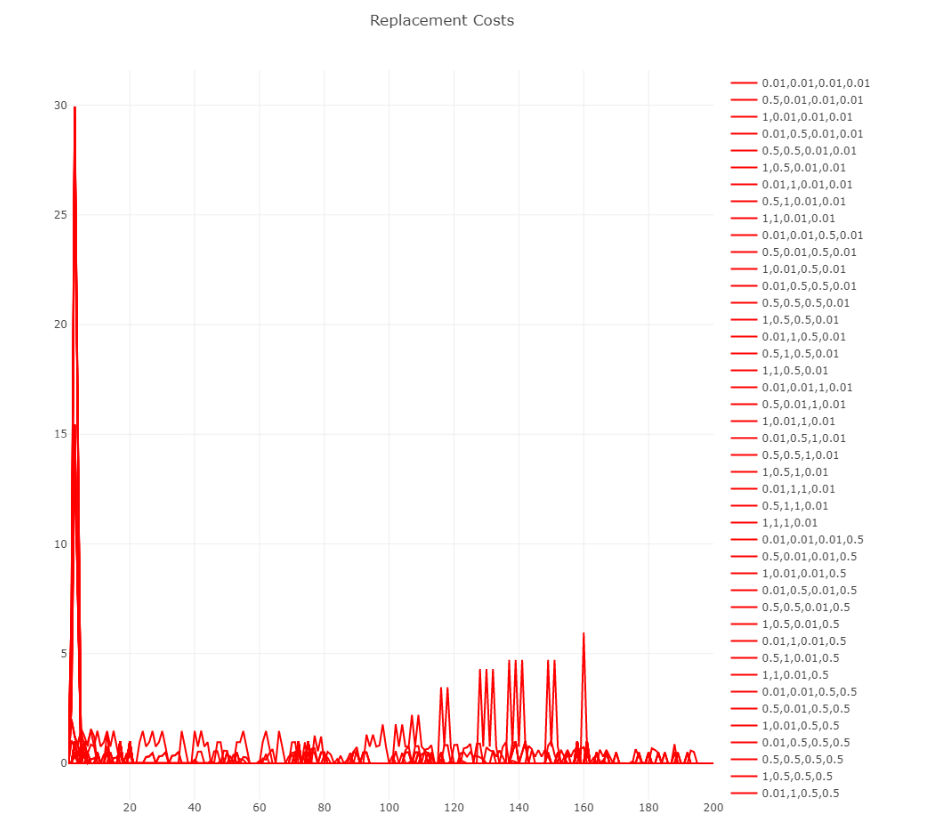
\includegraphics[scale=0.5]{./pictures/combination_experiment/replacement.png}
%\end{figure}
%\begin{figure}[h]
%	\centering
%	\caption{Experiment 2  - Taken Costs}
%	\label{addition_experiment_costs}
%	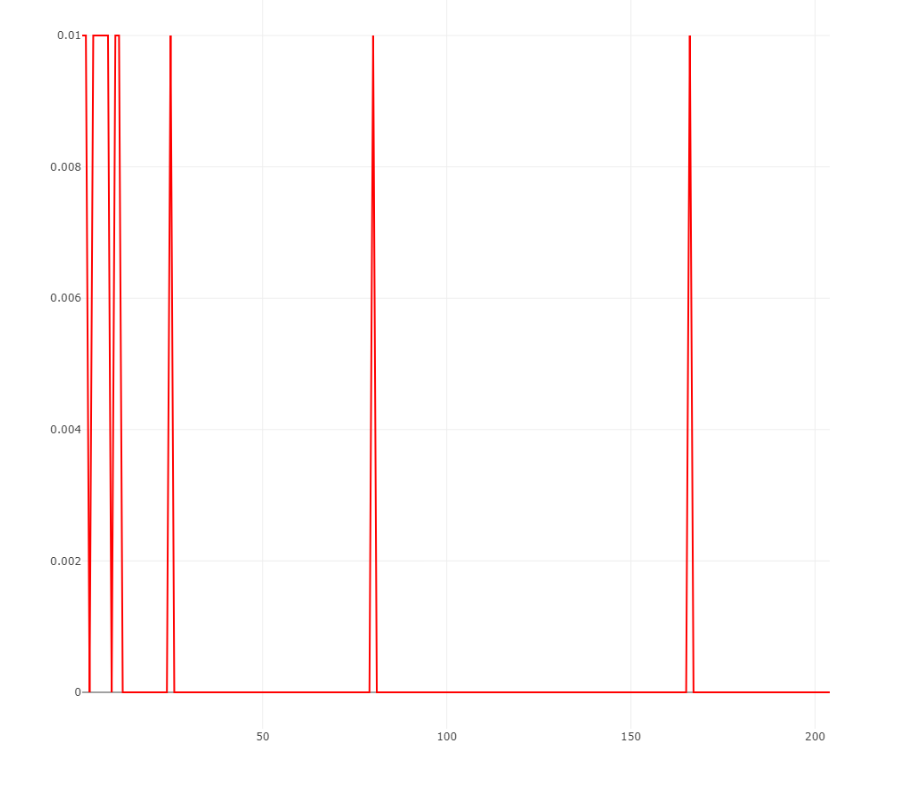
\includegraphics[scale=0.5]{./pictures/combination_experiment/costs.png}
%\end{figure}

\newpage
\subsubsection{Evaluation}
In the following tables we can see exactly which set of combination accomplished to learn the models mentioned previously. Each table will be analyzed separately and the conclusion of this experiment will be drawn until the end of this section.\\ \\
%
Let us first take a look when the original model could be learned completely in Table \ref{table:combination_1}. We can see that  the \textit{similarity threshold} never reached 1.0 and that the time constraints were given low priority at all times. In contrast to the \textit{location cost} which never reached the value of 0.1. It was for almost all of the cases that the model could be perfectly learned, by only giving priority to the functionalities of the observations and the overall number of nodes required to express observations. \\ \\
%
In Table \ref{table:combination_2} one can see the combinations when 70 \% of the model could be learned. It was the case that raising the priority of the \textit{time cost} had a negative effect on the learning process, despite the fact that the \textit{cost function} and \textit{location cost} remained relatively similar.  As seen in Figure \ref{combination_experiment_2}, this combination could not learned the model completely, only because two different time units of unique nodes were observed (nodes \textit{EQ7} and \textit{EQ9} from the same figure). \\ \\
%
At last, we will discuss Table \ref{table:combination_3}, were the worst combinations can be appreciated. In the majority of the cases, the model was wrongly learned whenever only identical observations were possible to merge (e.g. similarity threshold equal to 1). This is to be expected, as with a high \textit{similarity threshold}, the learned model does not tolerate any noisy or slightly modified observations. The same applies whenever the \textit{time cost} was set to a high value, as some of the observations had different time constraints and identical behaviors.  \\ \\
%
For this specific experiment, it was enough to ignore the minimal noise of the time constraints of the observations, and to separate the observations based on they're functionalities because they were relatively far between each other. 

\begin{table}[htbp]
	\centering
	\resizebox{0.8\textwidth}{!}{\begin{minipage}{\textwidth}
\begin{tabular}{||c c c c c||}
	\hline
	Similarity Threshold & Time Cost & Functionality Cost & Location Cost & Graph Similarity  \\ [0.5ex] 
	\hline\hline
	\hline
	0.1 & 0.1 & 0.1 & 0.5 & 1 \\ 
	\hline
	0.5 & 0.1 & 0.1 & 0.5 & 1 \\ 
	\hline
	0.1 & 0.1 & 0.5 & 0.5 & 1 \\ 
	\hline
	0.5 & 0.1 & 0.5 & 0.5 & 1 \\ 
	\hline
	0.1 & 0.1 & 1 & 0.5 & 1 \\ 
	\hline
	0.5 & 0.1 & 1 & 0.5 & 1 \\ 
	\hline
	0.1 & 0.1 & 0.1 & 1 & 1 \\
	\hline
	0.5 & 0.1 & 0.1 & 1 & 1 \\ 
	\hline
	0.1 & 0.1 & 0.5 & 1 & 1 \\ 
	\hline
	0.5 & 0.1 & 0.5 & 1 & 1 \\ 
	\hline
	0.1 & 0.1 & 1 & 1 & 1 \\ 
	\hline
	0.5 & 0.1 & 1 & 1 & 1 \\  [1ex] 
	\hline
\end{tabular}
 \end{minipage}}
\caption{Sub-Experiment 1 - Combinations that learned the complete model}
\label{table:combination_1}
\end{table}

\begin{table}[htbp]
	\centering
	\resizebox{0.8\textwidth}{!}{\begin{minipage}{\textwidth}
\begin{tabular}{||c c c c c||}
	\hline
	Similarity Threshold & Time Cost & Functionality Cost & Location Cost & Graph Similarity  \\ [0.5ex] 
	\hline\hline
	0.1 & 0.5 & 0.1 & 1 & 0.6999942199698811 \\ 
	\hline
	0.5 & 0.5 & 0.1 & 1 & 0.6999942199698811 \\ 
	\hline
	0.1 & 0.5 & 0.5 & 1 & 0.6999942199698811 \\ 
	\hline
	0.5 & 0.5 & 0.5 & 1 & 0.6999942199698811 \\ 
	\hline
	0.1 & 0.5 & 1 & 1 & 0.6999942199698811 \\ 
	\hline
	0.5 & 0.5 & 1 & 1 & 0.6999942199698811 \\ [1ex] 
	\hline 
\end{tabular}
 \end{minipage}}
\caption{Sub-Experiment 1- Combinations that learned 70\% of the model}
\label{table:combination_2}
\end{table}

\begin{table}[htbp]
	\centering
	\resizebox{0.5\textwidth}{!}{\begin{minipage}{\textwidth}
			\begin{tabular}{||c c c c c||}
				\hline
				Similarity Threshold & Time Cost & Functionality Cost & Location Cost & Graph Similarity  \\ [0.5ex] 
				\hline\hline
				0.1 & 0.1 & 0.1 & 0.1 & 0.545447328305253 \\ 
				\hline
				0.5 & 0.1 & 0.1 & 0.1 & 0.545447328305253 \\ 
				\hline
				1 & 0.1 & 0.1 & 0.1 & 0.545447328305253 \\ 
				\hline
				0.1 & 0.5 & 0.1 & 0.1 & 0.545447328305253 \\ 
				\hline
				0.5 & 0.5 & 0.1 & 0.1 & 0.545447328305253 \\ 
				\hline
				1 & 0.5 & 0.1 & 0.1 & 0.545447328305253 \\ 
				\hline
				0.1 & 1 & 0.1 & 0.1 & 0.545447328305253 \\ 
				\hline
				0.5 & 1 & 0.1 & 0.1 & 0.545447328305253 \\ 
				\hline
				1 & 1 & 0.1 & 0.1 & 0.545447328305253 \\ 
				\hline
				0.1 & 0.1 & 0.5 & 0.1 & 0.545447328305253 \\ 
				\hline
				0.5 & 0.1 & 0.5 & 0.1 & 0.545447328305253 \\ 
				\hline
				1 & 0.1 & 0.5 & 0.1 & 0.545447328305253 \\ 
				\hline
				0.1 & 0.5 & 0.5 & 0.1 & 0.545447328305253 \\ 
				\hline
				0.5 & 0.5 & 0.5 & 0.1 & 0.545447328305253 \\ 
				\hline
				1 & 0.5 & 0.5 & 0.1 & 0.545447328305253 \\ 
				\hline
				0.1 & 1 & 0.5 & 0.1 & 0.545447328305253 \\ 
				\hline
				0.5 & 1 & 0.5 & 0.1 & 0.545447328305253 \\ 
				\hline
				1 & 1 & 0.5 & 0.1 & 0.545447328305253 \\ 
				\hline
				0.1 & 0.1 & 1 & 0.1 & 0.545447328305253 \\ 
				\hline
				0.5 & 0.1 & 1 & 0.1 & 0.545447328305253 \\ 
				\hline
				1 & 0.1 & 1 & 0.1 & 0.545447328305253 \\ 
				\hline
				0.1 & 0.5 & 1 & 0.1 & 0.545447328305253 \\ 
				\hline
				0.5 & 0.5 & 1 & 0.1 & 0.545447328305253 \\ 
				\hline
				1 & 0.5 & 1 & 0.1 & 0.545447328305253 \\ 
				\hline
				0.1 & 1 & 1 & 0.1 & 0.545447328305253 \\ 
				\hline
				0.5 & 1 & 1 & 0.1 & 0.545447328305253 \\ 
				\hline
				1 & 1 & 1 & 0.1 & 0.545447328305253 \\ 
				\hline
				1 & 0.1 & 0.1 & 0.5 & 0.545447328305253 \\ 
				\hline
				0.1 & 0.5 & 0.1 & 0.5 & 0.545447328305253 \\ 
				\hline
				0.5 & 0.5 & 0.1 & 0.5 & 0.545447328305253 \\ 
				\hline
				1 & 0.5 & 0.1 & 0.5 & 0.545447328305253 \\ 
				\hline
				0.1 & 1 & 0.1 & 0.5 & 0.545447328305253 \\ 
				\hline
				0.5 & 1 & 0.1 & 0.5 & 0.545447328305253 \\ 
				\hline
				1 & 1 & 0.1 & 0.5 & 0.545447328305253 \\ 
				\hline
				1 & 0.1 & 0.5 & 0.5 & 0.545447328305253 \\ 
				\hline
				0.1 & 0.5 & 0.5 & 0.5 & 0.545447328305253 \\ 
				\hline
				0.5 & 0.5 & 0.5 & 0.5 & 0.545447328305253 \\ 
				\hline
				1 & 0.5 & 0.5 & 0.5 & 0.545447328305253 \\ 
				\hline
				0.1 & 1 & 0.5 & 0.5 & 0.545447328305253 \\ 
				\hline
				0.5 & 1 & 0.5 & 0.5 & 0.545447328305253 \\ 
				\hline
				1 & 1 & 0.5 & 0.5 & 0.545447328305253 \\ 
				\hline
				1 & 0.1 & 1 & 0.5 & 0.545447328305253 \\ 
				\hline
				0.1 & 0.5 & 1 & 0.5 & 0.545447328305253 \\ 
				\hline
				0.5 & 0.5 & 1 & 0.5 & 0.545447328305253 \\ 
				\hline
				1 & 0.5 & 1 & 0.5 & 0.545447328305253 \\ 
				\hline
				0.1 & 1 & 1 & 0.5 & 0.545447328305253 \\ 
				\hline
				0.5 & 1 & 1 & 0.5 & 0.545447328305253 \\ 
				\hline
				1 & 1 & 1 & 0.5 & 0.545447328305253 \\ 
				\hline
				1 & 0.1 & 0.1 & 1 & 0.545447328305253 \\ 
				\hline
				1 & 0.5 & 0.1 & 1 & 0.545447328305253 \\ 
				\hline
				0.1 & 1 & 0.1 & 1 & 0.545447328305253 \\ 
				\hline
				0.5 & 1 & 0.1 & 1 & 0.545447328305253 \\ 
				\hline
				1 & 1 & 0.1 & 1 & 0.545447328305253 \\ 
				\hline
				1 & 0.1 & 0.5 & 1 & 0.545447328305253 \\ 
				\hline
				1 & 0.5 & 0.5 & 1 & 0.545447328305253 \\ 
				\hline
				0.1 & 1 & 0.5 & 1 & 0.545447328305253 \\ 
				\hline
				0.5 & 1 & 0.5 & 1 & 0.545447328305253 \\ 
				\hline
				1 & 1 & 0.5 & 1 & 0.545447328305253 \\ 
				\hline
				1 & 0.1 & 1 & 1 & 0.545447328305253 \\
				\hline
				1 & 0.5 & 1 & 1 & 0.545447328305253 \\ 
				\hline
				0.1 & 1 & 1 & 1 & 0.545447328305253 \\ 
				\hline
				0.5 & 1 & 1 & 1 & 0.545447328305253 \\ 
				\hline
				1 & 1 & 1 & 1 & 0.545447328305253 \\  [1ex] 
				\hline
			\end{tabular}
	\end{minipage}}
	\caption{Sub-Experiment 1 - Combinations that learned 54\% of the model}
\label{table:combination_3}
\end{table}

\newpage

\subsection{Sub-Experiment 2}
This experiment was intended to briefly demonstrate how the incremental learning approach works with 2 simple models, under the same conditions as in Sub-Experiment 1. Meaning that we also learn all fo the upcoming models with the same 81 possible combinations of parameters. Due to the simplicity of the tested models, we first describe their structure in sub-section \textit{Model Description} and then we discuss the results in the sub-section \textit{Results}. 

\subsubsection{ Model Description }
The first model from Figure \ref{combination_experiment_simple_1} is a simple branched model with only two \textit{out-going} nodes coming from the same \textit{parent} and no further nodes. While the second model from Figure \ref{combination_experiment_simple_2} consists of three sequential nodes, where each node can only have one \textit{parent}.
\begin{figure}[t]
	\centering
	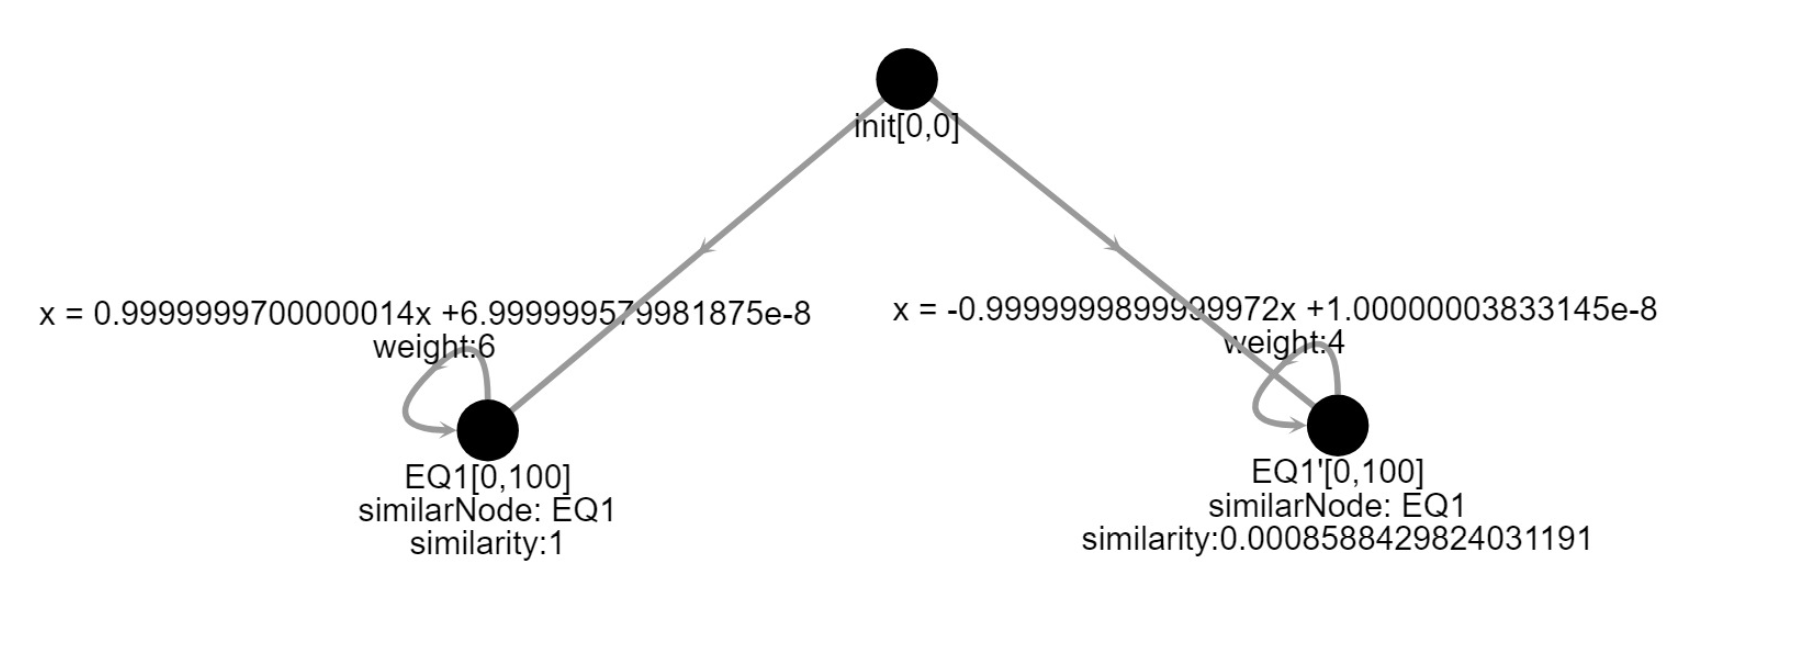
\includegraphics[scale=0.4]{./pictures/simple_experiment/learnedModel_branched_far.png}
	\caption{Sub-Experiment 2 - Branched Model}
	\label{combination_experiment_simple_1}
\end{figure}

\begin{figure}[h]
	\centering
	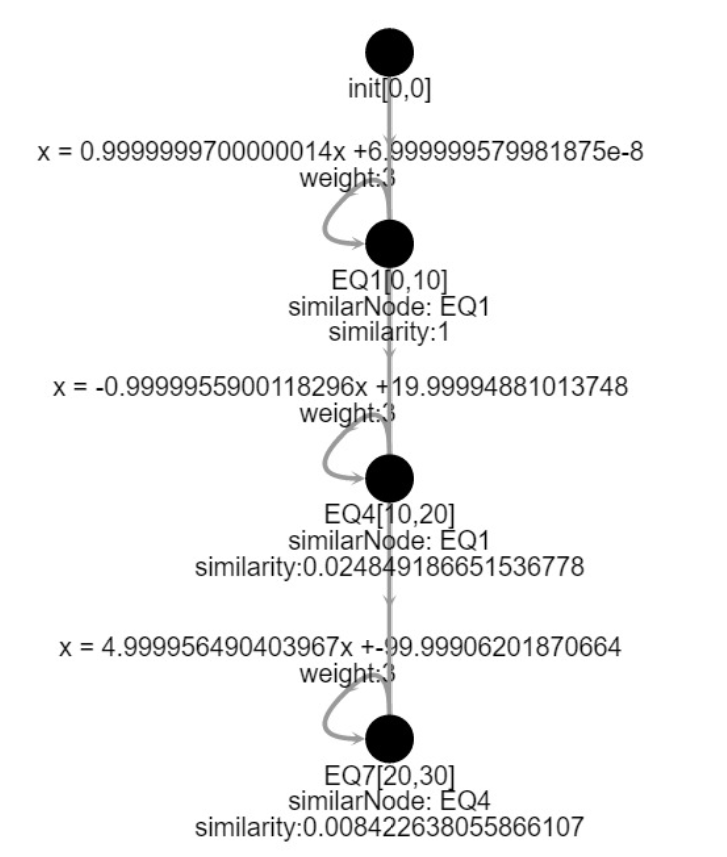
\includegraphics[scale=0.4]{./pictures/simple_experiment/learnedModel_sequential_far.png}
	\caption{Sub-Experiment 2 - Sequential Model}
	\label{combination_experiment_simple_2}
\end{figure}

\subsubsection{ Results}
We can see very positive results from both models in Table \ref{table:combination_simple_1} and Table \ref{table:combination_simple_2}, as it was always the case that the original models were sucessfully learned. This happens because the nodes from both models are relatively far and can be easily identified by the implementation with the calculation of their normalized Euclidean distances (e.g. similarity value). For example, one can see in Figure \ref{combination_experiment_simple_1} that the similarity value between \textit{EQ1} and \textit{EQ1'} is of approximately 0.00085. This value is always lower than the similarity threshold, as the last one can only be as low as 0.1. Meaning that the nodes from the previous models can never be merged, due to their difference in functionality. For this particular set of models, the only possibility to merge nodes would be to lower the similarity threshold from 0.1 to a value very close to 0. The only disadvantage of setting parameters like the \textit{similarity threshold} to 0, is that it may cause the learning process to loose significant precision of the observations. It may also confuse the learning process and indicate that very different nodes should be merged, when in reality they should be treated as different nodes.
\newpage
\begin{table}[htbp]
	\centering
	\resizebox{0.5\textwidth}{!}{\begin{minipage}{\textwidth}
			\begin{tabular}{||c c c c c||}
				\hline
				Similarity Threshold & Time Cost & Functionality Cost & Location Cost & Graph Similarity  \\ [0.5ex] 
				\hline\hline
				0.1 & 0.1 & 0.1 & 0.1 & 1 \\ 
				\hline
				0.5 & 0.1 & 0.1 & 0.1 & 1 \\ 
				\hline
				1 & 0.1 & 0.1 & 0.1 & 1 \\ 
				\hline
				0.1 & 0.5 & 0.1 & 0.1 & 1 \\ 
				\hline
				0.5 & 0.5 & 0.1 & 0.1 & 1 \\ 
				\hline
				1 & 0.5 & 0.1 & 0.1 & 1 \\ 
				\hline
				0.1 & 1 & 0.1 & 0.1 & 1 \\ 
				\hline
				0.5 & 1 & 0.1 & 0.1 & 1 \\ 
				\hline
				1 & 1 & 0.1 & 0.1 & 1 \\ 
				\hline
				0.1 & 0.1 & 0.5 & 0.1 & 1 \\ 
				\hline
				0.5 & 0.1 & 0.5 & 0.1 & 1 \\ 
				\hline
				1 & 0.1 & 0.5 & 0.1 & 1 \\ 
				\hline
				0.1 & 0.5 & 0.5 & 0.1 & 1 \\ 
				\hline
				0.5 & 0.5 & 0.5 & 0.1 & 1 \\ 
				\hline
				1 & 0.5 & 0.5 & 0.1 & 1 \\ 
				\hline
				0.1 & 1 & 0.5 & 0.1 & 1 \\ 
				\hline
				0.5 & 1 & 0.5 & 0.1 & 1 \\ 
				\hline
				1 & 1 & 0.5 & 0.1 & 1 \\ 
				\hline
				0.1 & 0.1 & 1 & 0.1 & 1 \\ 
				\hline
				0.5 & 0.1 & 1 & 0.1 & 1 \\ 
				\hline
				1 & 0.1 & 1 & 0.1 & 1 \\ 
				\hline
				0.1 & 0.5 & 1 & 0.1 & 1 \\ 
				\hline
				0.5 & 0.5 & 1 & 0.1 & 1 \\ 
				\hline
				1 & 0.5 & 1 & 0.1 & 1 \\ 
				\hline
				0.1 & 1 & 1 & 0.1 & 1 \\ 
				\hline
				0.5 & 1 & 1 & 0.1 & 1 \\ 
				\hline
				1 & 1 & 1 & 0.1 & 1 \\ 
				\hline
				0.1 & 0.1 & 0.1 & 0.5 & 1 \\ 
				\hline
				0.5 & 0.1 & 0.1 & 0.5 & 1 \\ 
				\hline
				1 & 0.1 & 0.1 & 0.5 & 1 \\ 
				\hline
				0.1 & 0.5 & 0.1 & 0.5 & 1 \\ 
				\hline
				0.5 & 0.5 & 0.1 & 0.5 & 1 \\ 
				\hline
				1 & 0.5 & 0.1 & 0.5 & 1 \\ 
				\hline
				0.1 & 1 & 0.1 & 0.5 & 1 \\ 
				\hline
				0.5 & 1 & 0.1 & 0.5 & 1 \\ 
				\hline
				1 & 1 & 0.1 & 0.5 & 1 \\ 
				\hline
				0.1 & 0.1 & 0.5 & 0.5 & 1 \\ 
				\hline
				0.5 & 0.1 & 0.5 & 0.5 & 1 \\ 
				\hline
				1 & 0.1 & 0.5 & 0.5 & 1 \\ 
				\hline
				0.1 & 0.5 & 0.5 & 0.5 & 1 \\ 
				\hline
				0.5 & 0.5 & 0.5 & 0.5 & 1 \\ 
				\hline
				1 & 0.5 & 0.5 & 0.5 & 1 \\ 
				\hline
				0.1 & 1 & 0.5 & 0.5 & 1 \\ 
				\hline
				0.5 & 1 & 0.5 & 0.5 & 1 \\ 
				\hline
				1 & 1 & 0.5 & 0.5 & 1 \\ 
				\hline
				0.1 & 0.1 & 1 & 0.5 & 1 \\ 
				\hline
				0.5 & 0.1 & 1 & 0.5 & 1 \\ 
				\hline
				1 & 0.1 & 1 & 0.5 & 1 \\ 
				\hline
				0.1 & 0.5 & 1 & 0.5 & 1 \\ 
				\hline
				0.5 & 0.5 & 1 & 0.5 & 1 \\ 
				\hline
				1 & 0.5 & 1 & 0.5 & 1 \\ 
				\hline
				0.1 & 1 & 1 & 0.5 & 1 \\ 
				\hline
				0.5 & 1 & 1 & 0.5 & 1 \\ 
				\hline
				1 & 1 & 1 & 0.5 & 1 \\ 
				\hline
				0.1 & 0.1 & 0.1 & 1 & 1 \\ 
				\hline
				0.5 & 0.1 & 0.1 & 1 & 1 \\ 
				\hline
				1 & 0.1 & 0.1 & 1 & 1 \\ 
				\hline
				0.1 & 0.5 & 0.1 & 1 & 1 \\ 
				\hline
				0.5 & 0.5 & 0.1 & 1 & 1 \\ 
				\hline
				1 & 0.5 & 0.1 & 1 & 1 \\ 
				\hline
				0.1 & 1 & 0.1 & 1 & 1 \\ 
				\hline
				0.5 & 1 & 0.1 & 1 & 1 \\ 
				\hline
				1 & 1 & 0.1 & 1 & 1 \\ 
				\hline
				0.1 & 0.1 & 0.5 & 1 & 1 \\ 
				\hline
				0.5 & 0.1 & 0.5 & 1 & 1 \\ 
				\hline
				1 & 0.1 & 0.5 & 1 & 1 \\ 
				\hline
				0.1 & 0.5 & 0.5 & 1 & 1 \\ 
				\hline
				0.5 & 0.5 & 0.5 & 1 & 1 \\ 
				\hline
				1 & 0.5 & 0.5 & 1 & 1 \\ 
				\hline
				0.1 & 1 & 0.5 & 1 & 1 \\ 
				\hline
				0.5 & 1 & 0.5 & 1 & 1 \\ 
				\hline
				1 & 1 & 0.5 & 1 & 1 \\ 
				\hline
				0.1 & 0.1 & 1 & 1 & 1 \\ 
				\hline
				0.5 & 0.1 & 1 & 1 & 1 \\ 
				\hline
				1 & 0.1 & 1 & 1 & 1 \\ 
				\hline
				0.1 & 0.5 & 1 & 1 & 1 \\ 
				\hline
				0.5 & 0.5 & 1 & 1 & 1 \\ 
				\hline
				1 & 0.5 & 1 & 1 & 1 \\ 
				\hline
				0.1 & 1 & 1 & 1 & 1 \\ 
				\hline
				0.5 & 1 & 1 & 1 & 1 \\ 
				\hline
				1 & 1 & 1 & 1 & 1 \\ [1ex] 
				\hline
				\hline
			\end{tabular}
	\end{minipage}}
	\caption{Sub-Experiment 2 - Branched Model Results}
	\label{table:combination_simple_1}
\end{table}

\begin{table}[htbp]
	\centering
	\resizebox{0.5\textwidth}{!}{\begin{minipage}{\textwidth}
			\begin{tabular}{||c c c c c||}
				\hline
				Similarity Threshold & Time Cost & Functionality Cost & Location Cost & Graph Similarity  \\ [0.5ex] 
				\hline\hline
				0.1 & 0.1 & 0.1 & 0.1 & 1 \\ 
				\hline
				0.5 & 0.1 & 0.1 & 0.1 & 1 \\ 
				\hline
				1 & 0.1 & 0.1 & 0.1 & 1 \\ 
				\hline
				0.1 & 0.5 & 0.1 & 0.1 & 1 \\ 
				\hline
				0.5 & 0.5 & 0.1 & 0.1 & 1 \\ 
				\hline
				1 & 0.5 & 0.1 & 0.1 & 1 \\ 
				\hline
				0.1 & 1 & 0.1 & 0.1 & 1 \\ 
				\hline
				0.5 & 1 & 0.1 & 0.1 & 1 \\ 
				\hline
				1 & 1 & 0.1 & 0.1 & 1 \\ 
				\hline
				0.1 & 0.1 & 0.5 & 0.1 & 1 \\ 
				\hline
				0.5 & 0.1 & 0.5 & 0.1 & 1 \\ 
				\hline
				1 & 0.1 & 0.5 & 0.1 & 1 \\ 
				\hline
				0.1 & 0.5 & 0.5 & 0.1 & 1 \\ 
				\hline
				0.5 & 0.5 & 0.5 & 0.1 & 1 \\ 
				\hline
				1 & 0.5 & 0.5 & 0.1 & 1 \\ 
				\hline
				0.1 & 1 & 0.5 & 0.1 & 1 \\ 
				\hline
				0.5 & 1 & 0.5 & 0.1 & 1 \\ 
				\hline
				1 & 1 & 0.5 & 0.1 & 1 \\ 
				\hline
				0.1 & 0.1 & 1 & 0.1 & 1 \\ 
				\hline
				0.5 & 0.1 & 1 & 0.1 & 1 \\ 
				\hline
				1 & 0.1 & 1 & 0.1 & 1 \\ 
				\hline
				0.1 & 0.5 & 1 & 0.1 & 1 \\ 
				\hline
				0.5 & 0.5 & 1 & 0.1 & 1 \\ 
				\hline
				1 & 0.5 & 1 & 0.1 & 1 \\ 
				\hline
				0.1 & 1 & 1 & 0.1 & 1 \\ 
				\hline
				0.5 & 1 & 1 & 0.1 & 1 \\ 
				\hline
				1 & 1 & 1 & 0.1 & 1 \\ 
				\hline
				0.1 & 0.1 & 0.1 & 0.5 & 1 \\ 
				\hline
				0.5 & 0.1 & 0.1 & 0.5 & 1 \\ 
				\hline
				1 & 0.1 & 0.1 & 0.5 & 1 \\ 
				\hline
				0.1 & 0.5 & 0.1 & 0.5 & 1 \\ 
				\hline
				0.5 & 0.5 & 0.1 & 0.5 & 1 \\ 
				\hline
				1 & 0.5 & 0.1 & 0.5 & 1 \\ 
				\hline
				0.1 & 1 & 0.1 & 0.5 & 1 \\ 
				\hline
				0.5 & 1 & 0.1 & 0.5 & 1 \\ 
				\hline
				1 & 1 & 0.1 & 0.5 & 1 \\ 
				\hline
				0.1 & 0.1 & 0.5 & 0.5 & 1 \\ 
				\hline
				0.5 & 0.1 & 0.5 & 0.5 & 1 \\ 
				\hline
				1 & 0.1 & 0.5 & 0.5 & 1 \\ 
				\hline
				0.1 & 0.5 & 0.5 & 0.5 & 1 \\ 
				\hline
				0.5 & 0.5 & 0.5 & 0.5 & 1 \\ 
				\hline
				1 & 0.5 & 0.5 & 0.5 & 1 \\ 
				\hline
				0.1 & 1 & 0.5 & 0.5 & 1 \\ 
				\hline
				0.5 & 1 & 0.5 & 0.5 & 1 \\ 
				\hline
				1 & 1 & 0.5 & 0.5 & 1 \\ 
				\hline
				0.1 & 0.1 & 1 & 0.5 & 1 \\ 
				\hline
				0.5 & 0.1 & 1 & 0.5 & 1 \\ 
				\hline
				1 & 0.1 & 1 & 0.5 & 1 \\ 
				\hline
				0.1 & 0.5 & 1 & 0.5 & 1 \\ 
				\hline
				0.5 & 0.5 & 1 & 0.5 & 1 \\ 
				\hline
				1 & 0.5 & 1 & 0.5 & 1 \\ 
				\hline
				0.1 & 1 & 1 & 0.5 & 1 \\ 
				\hline
				0.5 & 1 & 1 & 0.5 & 1 \\ 
				\hline
				1 & 1 & 1 & 0.5 & 1 \\ 
				\hline
				0.1 & 0.1 & 0.1 & 1 & 1 \\ 
				\hline
				0.5 & 0.1 & 0.1 & 1 & 1 \\ 
				\hline
				1 & 0.1 & 0.1 & 1 & 1 \\ 
				\hline
				0.1 & 0.5 & 0.1 & 1 & 1 \\ 
				\hline
				0.5 & 0.5 & 0.1 & 1 & 1 \\ 
				\hline
				1 & 0.5 & 0.1 & 1 & 1 \\ 
				\hline
				0.1 & 1 & 0.1 & 1 & 1 \\ 
				\hline
				0.5 & 1 & 0.1 & 1 & 1 \\ 
				\hline
				1 & 1 & 0.1 & 1 & 1 \\ 
				\hline
				0.1 & 0.1 & 0.5 & 1 & 1 \\ 
				\hline
				0.5 & 0.1 & 0.5 & 1 & 1 \\ 
				\hline
				1 & 0.1 & 0.5 & 1 & 1 \\ 
				\hline
				0.1 & 0.5 & 0.5 & 1 & 1 \\ 
				\hline
				0.5 & 0.5 & 0.5 & 1 & 1 \\ 
				\hline
				1 & 0.5 & 0.5 & 1 & 1 \\ 
				\hline
				0.1 & 1 & 0.5 & 1 & 1 \\ 
				\hline
				0.5 & 1 & 0.5 & 1 & 1 \\ 
				\hline
				1 & 1 & 0.5 & 1 & 1 \\ 
				\hline
				0.1 & 0.1 & 1 & 1 & 1 \\ 
				\hline
				0.5 & 0.1 & 1 & 1 & 1 \\ 
				\hline
				1 & 0.1 & 1 & 1 & 1 \\ 
				\hline
				0.1 & 0.5 & 1 & 1 & 1 \\ 
				\hline
				0.5 & 0.5 & 1 & 1 & 1 \\ 
				\hline
				1 & 0.5 & 1 & 1 & 1 \\ 
				\hline
				0.1 & 1 & 1 & 1 & 1 \\ 
				\hline
				0.5 & 1 & 1 & 1 & 1 \\ 
				\hline
				1 & 1 & 1 & 1 & 1 \\ [1ex] 
				\hline
				\hline
			\end{tabular}
	\end{minipage}}
	\caption{Sub-Experiment 2 - Sequential Model Results}
	\label{table:combination_simple_2}
\end{table}

 
	
	\chapter{Conclusion and Future Work}
	\label{chap:futureWork}
	Learning probabilistic timed automata was possible by measuring observations incrementally, with the use of Euclidean distances and cost functions. 
%
As demonstrated in the experiments, we can find some optimal combinations for which the incremental learning approach works properly.
% 
Unfortunately, the implementation and concept of this approach is not able to detect optimal combinations on the fly. 
%
Nevertheless, it would be possible to also adapt parameters of the cost function and the similarity threshold incrementally, as we also measure graph similarity simultaneously. 
%
Another remark to take into consideration, is that our approach is able to detect noisy observations. The only disadvantage is that it is impossible to track whether noisy observations truly come from a trace of an automaton, or if the implementation did not receive enough information from the model to learn appropriately, as there is no interaction with the observed automaton like in active learning. Meaning that we do not allow to check properties of the model and are not able to verify which type of traces the observed model is able to emit. 
%
Disregarding the lack of communication with the model to be learned and assuming that it provides accurate observations. We can recreate precise models by analyzing and measuring observations in an incremental fashion. Unfortunately, further experiments must be done to prove that we can extend this approach to more complex types of timed automata, like probabilistic timed automata with cyclic behaviors. \\\\
%
One of the future concepts that can be applied to extend this approach is \textit{automata minimization}. An automaton is minimal, when there is no other automaton that accepts the same language with less locations. Working with a fixed number of locations would ensure having a canonical representation of automata, thus reducing complexity and ambiguities while learning and matching models.
%
The incremental learning approach developed only considers the modification of a single close node based on an observation, a cost functions and a similarity threshold. 
%
We could extend the concept of incremental learning to create graph reduction routines which would mainly consist of evaluating the cost of eliminating nodes by merging their functionality and time constraints with other similar nodes based on how close they are (e.g. By using different similarity threshold values). 
%
As we have seen, replacement of nodes involves the possible propagation of errors. Being that said, we would need to consider two main types of graph reduction routines: \textit{sequential merge} and \textit{parallel merge}.
%
A sequential merge would be done by merging sequential nodes. Specifically, pairs of nodes that do not belong to the same \textit{depth} of the graph, or when one node is \textit{parent} of the other. Whereas in parallel merge, the merge of nodes would be in the same depth of the graph, meaning that nodes might not be directly connected, consequently causing different propagation effects as in a sequential merge. 
%
The way that this approach would work, is by performing the reduction routines whenever there exists more locations in the learned model than in the original one. As we can already identify noisy observations and refer to the number of nodes of the original model, this extension is feasible and applicable to the implementation of this project. \\ \\ 

	
%	\chapter{Conclusion}
%	\label{chap:conclusion}
%	\input{./theory/10.Conclusion/conclusion.tex}
	
%	\appendix
%	\chapter{Listings}
%	\backmatter
	
%	\chapter{Bibliography}
	\bibliographystyle{plain}
	\bibliography{sample}
		
%	\begin{frame}
%	\frametitle{References}
    \nocite{*}
%	\renewcommand*{\bibfont}{\scriptsize}
%	\bibliographystyle{plain}

%	\end{frame}
%\appendix
%\section{UPPAAL Simulations}
%\label{appendix}
%%\begin{figure}[h]
%	\centering
%	\caption{Uppaal Simulation Trace Graph}
%	\label{uppaal_Simulation_Graph}
%	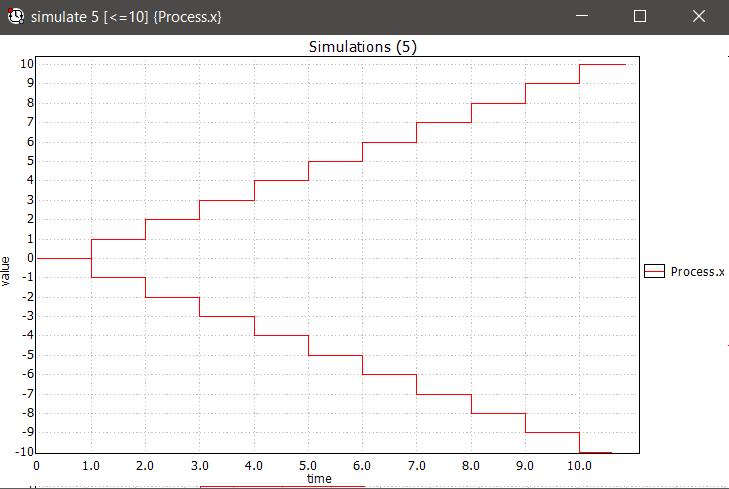
\includegraphics[scale=0.6]{./pictures/uppaal_model_example_simulation.png}
%\end{figure}
%
%\begin{figure}[h]
%	\centering
%	\caption{Uppaal Simulation Trace Data}
%	\label{uppaal_Simulation_Trace}
%	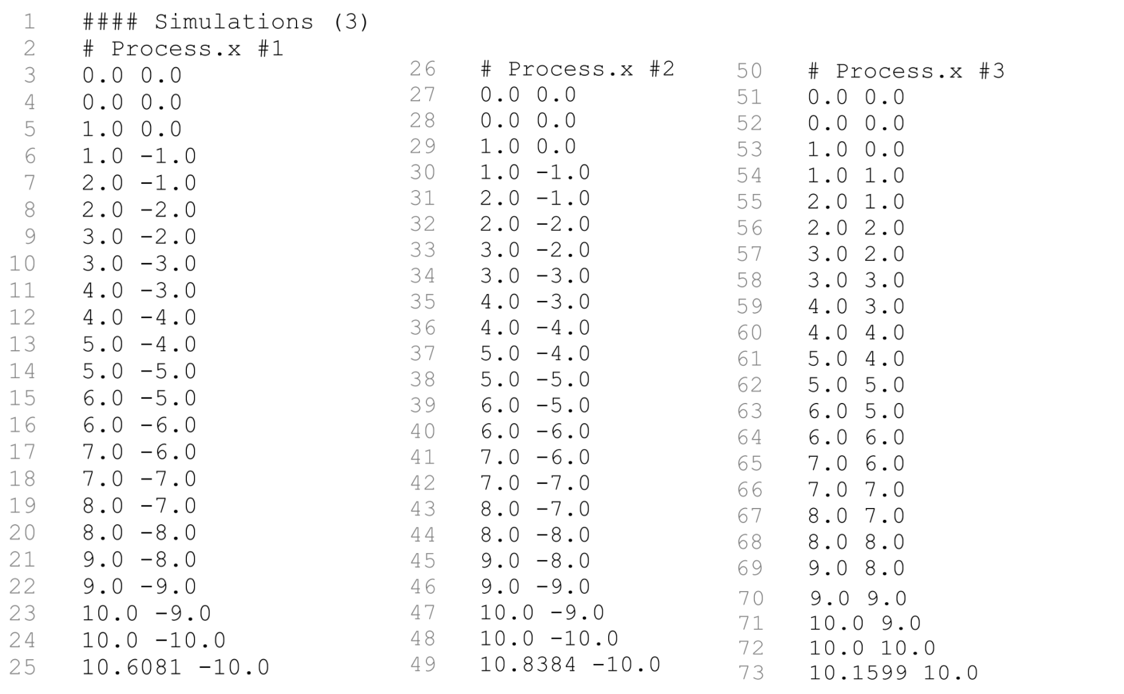
\includegraphics[scale=0.5]{./pictures/simulation_trace.png}
%\end{figure}
%

	
\end{document}
